\chapter{隐私保护密度聚类方案研究}
\section{引言}
% 1.说明隐私保护K-means研究存在的问题
%海量可获取的数据以及云计算提供的计算能力驱动机器学习的快速发展。有监督学习例如神经网络,使用带标签的数据来训练具有识别能力的模型。与之相反的是无监督学习,没有训练模型的过程,旨在从未标记的数据中发现未知的模式和特征。聚类是一种广泛使用的无监督机器学习工具,能够将相似的数据划分到同一个集合中。实际应用中,聚类常用于许多数据安全极为重要的领域,例如商业数据分析,市场数据挖掘以及医院病理信息分析等。上述场景中,数据一旦泄露会造成极大经济损失。
%
%目前,已有许多关于隐私保护聚类方案的研究,其中数量最多的是与K-means相关的研究\cite{hegde2021sok}。然而K-means聚类过程相对比较简单,并且只能检测到凸型簇,因此适用数据集类型极为受限。此外,簇的数量$k$必须要根据专业领域知识提前给出,如果只了解数据集的子集难以确定$k$的值。同时,K-means聚类不包含噪声的概念,并且聚类的结果对异常值非常敏感因为每一个输入都要被划分到某一个簇中。因此,即便某个输入不属于任何一个簇,它都会被划分到距离最近的簇,影响该簇的中心位置(簇中所有数据的平均值)。
%
%% 2.隐私保护DBSCAN的好处
%为了解决上述隐私保护方案中存在的问题,这里我们引入对隐私保护Density-based spatial clustering of applications with noise(DBSCAN)的研究。DBSCAN是一种由论文\cite{ester1996density}提出的更加灵活的聚类算法,能够检测到任意形状的簇。此外,簇的数量是根据数据集的特点灵活产生的,无需人工确定。该算法对异常值不敏感,会将其标记为噪声。本章首先提出了方案一,一种安全高效的隐私保护DBSCAN方案,该方案针对明文算法进行改进以适应安全计算的特点,将复杂度降低为$O(n^2)$,显著降低聚类所需时间。
%
%传统DBSCAN方案存在数据划分结果不稳定的问题,即最终划分结果取决于算法运行中数据遍历的顺序,将数据打乱后重新进行聚类,同一个点可能会被划分到不同的簇中。为了解决该问题,在论文\cite{tran2013revised}论文思想的基础上,我们在方案二中提出了改进的隐私保护DBSCAN,以获取稳定的聚类结果。
%
%尽管DBSCAN具有诸多优点,其聚类过程涉及两个重要参数minPts和$\epsilon$,这两个参数的取值与数据分布密切相关,通常需要人工分析后给出。为解决该问题,在论文\cite{latifi2021dbhc}的基础上,我们在方案三中提出了基于DBSCAN的隐私保护层次聚类,借助k近邻算法和k线图来决定聚类参数,并进行多轮聚类来适应不同密度的簇。
%% 3.本章组织结构
%本章的组织结构如下:第\ref{s4-yubei}节介绍了DBSCAN的相关内容。第\ref{s4-wenti}节中描述了系统模型、安全模型以及设计目标。第\ref{s4-subpro}节中增加了一些基于秘密共享的隐私保护计算模块。第\ref{s4-t1}节对隐私保护DBSCAN方案进行了详细介绍。第\ref{s4-t2}节中提出了方案二改进的隐私保护DBSCAN方案。第\ref{s4-t3}节中阐述了基于DBSCAN的隐私保护层次聚类方案。
%%第\ref{s4-lilun}节中从理论上分析了方案的正确性和安全性。、
%第\ref{s4-shiyan}节中对方案进行了实验评估。最后,在\ref{s4-xiaojie}节对本章进行了总结。

目前,已有许多关于隐私保护聚类方案的研究,其中数量最多的是与K-means相关的隐私保护研究\cite{hegde2021sok}。然而,K-means聚类存在诸多限制与缺点,其计算过程相对比较简单、聚类结果受到初始簇中心影响较大并且只能检测到凸型簇,因此适用场景极其有限。此外,簇的数量$k$必须要根据专业领域知识提前给出,如果只了解数据集的子集难以确定$k$的值。同时,K-means聚类不包含噪声的概念,聚类的结果对异常值非常敏感,因为每一个输入都要被划分到某一个簇中,影响该簇中心的位置(簇中所有数据的平均值)。

因此,一些研究人员转向基于DBSCAN的隐私保护聚类方案研究。DBSCAN是一种由Ester等人\cite{ester1996density}提出的更加灵活的聚类算法,能够检测到任意形状的簇。此外,簇的数量根据数据集的特点灵活产生,无需人工确定。该算法对异常值不敏感,会将其标记为噪声。关于隐私保护DBSCAN的相关研究相对较少,Rahman等人\cite{rahman2017towards}基于同态加密技术提出了一种外包隐私保护DBSCAN聚类方案,然而该方案泄露了簇大小和数据相邻关系,存在安全隐患。Bozdemir等人\cite{bozdemir2021privacy}基于ABY安全计算框架提出了一种高效的隐私保护DBSCAN方案,显著提升了聚类的效率减少了耗时,但是方案设计不够完善,引入了人工设置参数。
%同时,前述隐私保护K-means聚类方案不支持多用户上传数据进行协同聚类的场景,阻断了不同机构之间合作的桥梁,不利于提升聚类结果的质量。

% 2.隐私保护DBSCAN的好处
为了解决上述问题,本文提出了三种不同的隐私保护DBSCAN聚类方案,分别解决了不同的问题。方案一是一种安全高效的隐私保护DBSCAN方案,该方案设计了全新的隐私保护聚类协议,对比同类研究将密文方案复杂度降低为$O(n^2)$,显著降低聚类所需时间。传统DBSCAN方案存在数据划分结果不稳定的问题,即最终划分结果取决于算法运行中数据遍历的顺序,将数据打乱后重新进行聚类,同一个数据可能会被划分到不同的簇中。论文\cite{tran2013revised}在明文上提出改进的DBSCAN聚类方案解决了该问题,基于此,本文在方案二中提出了改进的隐私保护DBSCAN,以获取稳定的密文划分结果,提升密文聚类质量。尽管DBSCAN具有诸多优点,其聚类过程涉及两个重要参数minPts和$\epsilon$,这两个参数的取值与数据分布密切相关,通常需要人工分析后给出。论文\cite{latifi2021dbhc}在明文上借助k近邻算法和k线图来决定聚类参数,并进行多轮聚类来适应不同密度的簇,基于该方案的核心思想,本文在方案三中提出了基于DBSCAN的隐私保护层次聚类,以获取尽可能全面的聚类结果,提高算法对于数据集的适应性。

% 3.本章组织结构
本章的组织结构如下:第\ref{s4-yubei}节介绍了DBSCAN的相关内容。第\ref{s4-wenti}节中描述了系统模型、安全模型、设计目标以及系统输入。第\ref{s4-subpro}节中详细介绍了安全排序协议。第\ref{s4-t1}节对方案一隐私保护DBSCAN方案进行了详细介绍。第\ref{s4-t2}节中提出了方案二改进的隐私保护DBSCAN方案。第\ref{s4-t3}节中阐述了方案三基于DBSCAN的隐私保护层次聚类方案。
%第\ref{s4-lilun}节中从理论上分析了方案的正确性和安全性。、
第\ref{s4-shiyan}节中对方案进行了实验评估。最后,在\ref{s4-xiaojie}节对本章进行了总结。

\section{预备知识}
\label{s4-yubei}
本节主要介绍聚类质量衡量指标调整兰德系数、DBSCAN的明文算法、改进的DBSCAN算法以及基于DBSCAN的层次聚类方案。

\subsection{调整兰德系数}
\label{s4-ari-intro}
%参考了这里https://blog.csdn.net/sinat_30203515/article/details/82634778
调整兰德系数(Adjusted Rand Index,ARI)\cite{hubert1985comparing}用于评估聚类模型的性能,它的前身是兰德系数(Rand Index,RI)。
兰德系数的取值范围为$ [0,1] $,值越大意味着聚类结果与真实划分情况越吻合。
假设$ U $为外部评价标准(即真实划分结果),而$ V $为聚类结果,这里设定4个不同统计量:
\begin{compactitem}
	\item $ a $为在$ U $为同一类,在$ V $也为同一类别的数据元素对数。
	\item $ b $为在$ U $中为同一类,但在$ V $中属于不同类别的数据元素对数。
	\item $ c $为在$ U $中不在同一类,但在$ V $中为同一类别的数据元素对数。
	\item $ d $为在$ U $中不在同一类,且在$ V $中也不属于同一类别的数据元素对数。
\end{compactitem}

具体情况可以由表格\ref{ri-table}概括:

\begin{table}[htbp]
	\centering
	\renewcommand{\arraystretch}{1.3}
	\caption{RI指标计算参数解释}
	\scalebox{1.0}{
		\begin{tabular}{c|c|c|c}% 通过添加 | 来表示是否需要绘制竖线c|
			\hline  % 在表格最上方绘制横线
			分类   & 同一簇  & 不同簇  & 累加        \\
			\hline
			同一簇 & $ a $   & $ b $   & $ a+b $     \\
			\hline
			不同簇 & $ c $   & $ d $   & $ c+d $     \\
			\hline
			累加值 & $ a+c $ & $ b+d $ & $ a+b+c+d $ \\
			\hline
		\end{tabular}
	}
	\label{ri-table}
\end{table}

因此,最终兰德系数计算方式如公式\ref{ri}所示:
\begin{equation}
	R I=\frac{a+d}{a+b+c+d}
	\label{ri}
\end{equation}

然而上述计算方式无法保证随机划分的聚类结果RI值接近0,因此Hubert和Arabie等人在1985年提出了调整兰德系数。
下面给出该指标的计算方式,首先构造表格\ref{s4-table-ari},其中值$ n_{ij} $表示数据集中数据同时位于簇$ X $和簇$ Y $的个数。

\begin{table}[htbp]
	\centering
	\renewcommand{\arraystretch}{1.3}
	\caption{ARI指标计算中间值}
	\scalebox{1.0}{
		\begin{tabular}{|c|c|c|c|c|c|}% 通过添加 | 来表示是否需要绘制竖线c|
			\hline  % 在表格最上方绘制横线
			分类      & $ Y_1$     & $ Y_2 $    & $ \dots $ & $Y_s$      & 累加值    \\
			\hline
			$X_1$     & $ n_{11} $ & $ n_{12} $ & $ \dots $ & $ n_{1s} $ & $ a_1 $   \\
			\hline
			$ X_2 $   & $ n_{21} $ & $ n_{22} $ & $ \dots $ & $ n_{2s} $ & $ a_2 $   \\
			\hline
			$ \dots $ & $ \dots $  & $ \dots $  & $ \dots $ & $ \dots $  & $ \dots $ \\
			\hline
			$ X_r $   & $ n_{r1} $ & $ n_{r2} $ & $ \dots $ & $ n_{rs} $ & $a_r$     \\
			\hline
			累加值    & $ b_1 $    & $ b_2 $    & $ \dots $ & $ b_s $    &           \\
			\hline
		\end{tabular}
	}
	\label{s4-table-ari}
\end{table}

ARI的计算方式如公式\ref{equ_ari}所示,ARI的范围为$ [-1,1] $,该值越大则意味着聚类结果与正确划分结果越吻合。

\begin{equation}
	ARI = \frac{\sum_{i j}\left(\begin{array}{c}
				n_{i j} \\
				2
			\end{array}\right)-\left[\sum_i\left(\begin{array}{c}
				a_i \\
				2
			\end{array}\right) \sum_j\left(\begin{array}{c}
				b_j \\
				2
			\end{array}\right)\right] /\left(\begin{array}{c}
				n \\
				2
			\end{array}\right)}{\frac{1}{2}\left[\sum_i\left(\begin{array}{c}
				a_i \\
				2
			\end{array}\right)+\sum_j\left(\begin{array}{c}
				b_j \\
				2
			\end{array}\right)\right]-\left[\sum_i\left(\begin{array}{c}
				a_i \\
				2
			\end{array}\right) \sum_j\left(\begin{array}{c}
				b_j \\
				2
			\end{array}\right)\right] /\left(\begin{array}{c}
				n \\
				2
			\end{array}\right)}
	\label{equ_ari}
\end{equation}

ARI衡量指标的优点主要有,对于任意数量的聚类中心和样本数量,随机聚类结果的ARI值均非常接近于0,同时还可以用于比较不同聚类算法的效果差异。但是缺点也非常明显,计算该值需要已知数据集正确划分结果。


\subsection{DBSCAN}
DBSCAN是一种基于密度的聚类算法,在密集区域聚集在一起的数据点被划分到同一个簇中,稀疏区域的数据被标记为噪声\cite{khan2014dbscan}。算法要求两个重要参数:
\begin{compactitem}
	\item \textbf{$\epsilon$:} 也称为eps,确定两个点被视为相邻的最大距离。
	\item \textbf{minPts:} 确定邻域内至少包含多少点才能构成一个核心对象。
\end{compactitem}

DBSCAN围绕每个数据点以$\epsilon$为半径构建圈,并将数据点划分为核心点、边界点以及噪声点。若数据点$ \epsilon $范围内包含点的数量至少为minPts个,则认为是核心点。核心点邻域范围内的非核心点为边界点。若不属于上述任意一种情况,则为噪声点。围绕上述定义展开,DBSCAN还包含如下概念:

假设样本集为$D=(x_1,x_2,...,x_m)$:
\begin{compactitem}
	\item \textbf{密度直达:} 若$ x_i $位于$ x_j $的$ \epsilon$邻域内,且$ x_j $为核心对象,则称$ x_i $由$ x_j $密度直达,反之不一定成立。
	\item \textbf{密度可达:} 对于$ x_i $和$ x_j $,若存在样本序列$ p_1,p2,...,p_t $,满足$ p_1=x_i,p_T=x_j $,且$ p_{t+1} $由$ p_t $密度直达,则称$ x_j $由$ x_i $密度可达。
	\item \textbf{密度相连:} 对于$ x_i $和$ x_j $,如果存在核心点$ x_k $,使得$ x_i $和$ x_j $均由$ x_k $密度可达,则称$ x_i $和$ x_j $密度相连。
\end{compactitem}

\begin{figure}[htbp] %[htbp]
	\centering
	%	\captionsetup{font=scriptsize}
	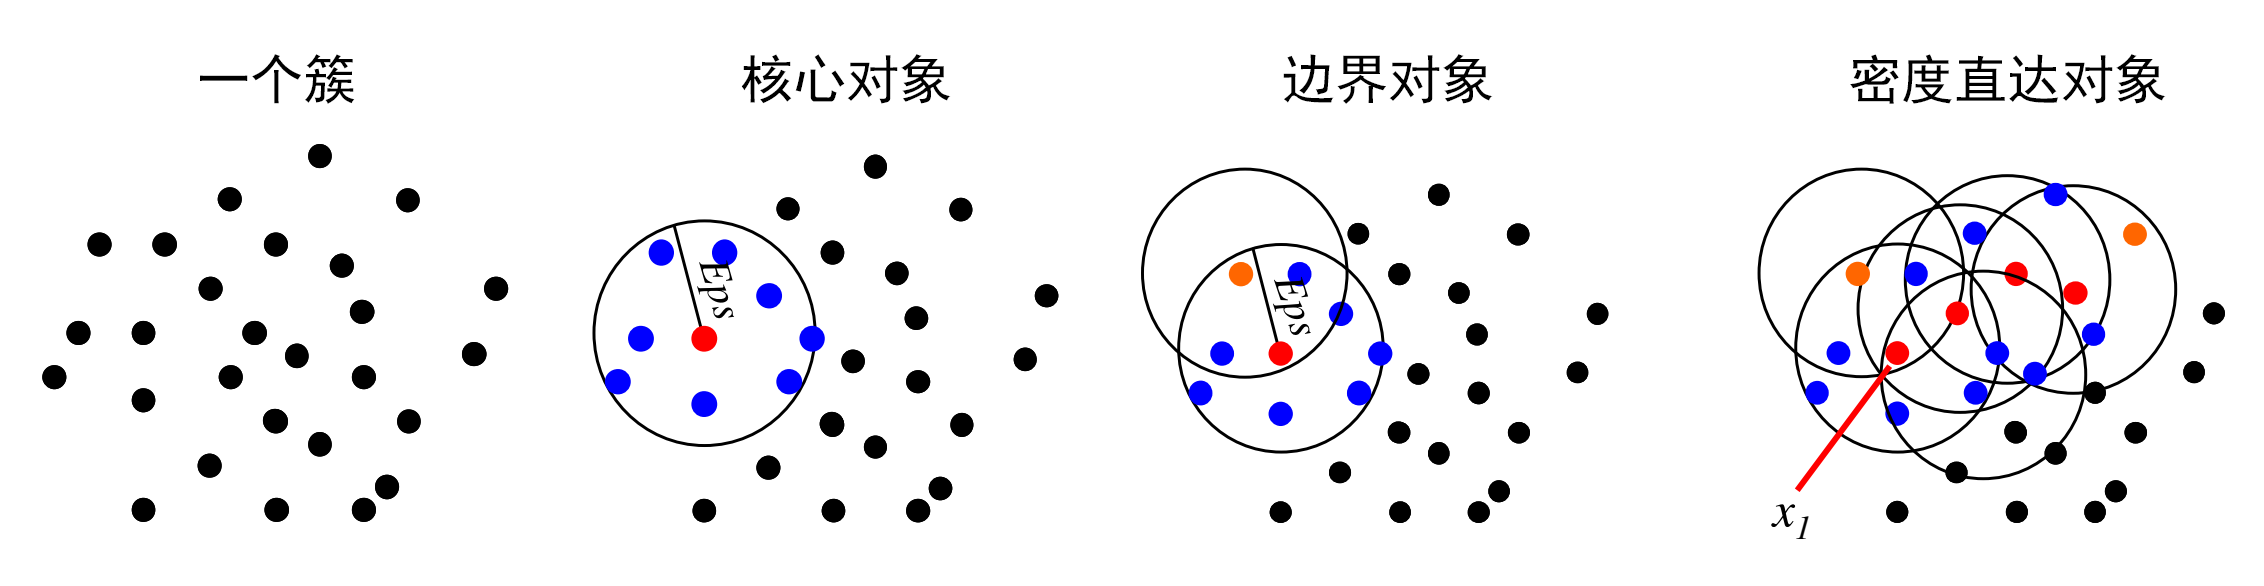
\includegraphics[scale=0.18 ]{img/dbscan-pre.png}
	\caption{DBSCAN相关概念可视化}
	\label{s4-dbscanpre}
\end{figure}

下面具体阐述DBSCAN聚类算法的流程:

\begin{enumerate}
	\item 初始化核心点集合$ \Omega = \varnothing  $,初始化簇数量$ k=0 $,初始化未访问点集合$ \Gamma = D $,簇划分$ C=\varnothing $
	\item 遍历所有点$ i=1,2,...,m $,按如下方式找到所有核心点:
	      \begin{enumerate}
		      \item 计算距离,找到样本$ x_i $的$ \epsilon- $邻域内所有点集合$ N_{\epsilon}(x_i) $
		      \item 如果集合包含数据点个数满足$ |N_{\epsilon}(x_i)| \geq minPts $,将$ x_i $加入核心点集合:$ \Omega = \Omega \cup \{x_j\} $
	      \end{enumerate}
	\item 若$ \Omega = \varnothing $,则算法结束,否则转入步骤4
	\item 在$ \Omega $中,随机选择一核心点$ o $,初始化当前簇包含核心点集合$ \Omega_{c}=\{o\} $,簇序号为$ k=k+1 $,当前簇包含点集合$ C_k=\{o\} $,更新未访问样本集合$ \Gamma = \Gamma - \{o\} $
	\item 若$ \Omega_{cur} = \varnothing $, 则簇$ C_k $聚类完毕,更新簇集合$ C=\{C_1,C_2,...,C_k\} $,更新核心点集合$ \Omega = \Omega - C_k $
	\item 从$ \Omega_{cur} $中取出一个核心点$ o' $,通过邻域距离$ \epsilon $找到所有$ \epsilon- $邻域子集$ N_{\epsilon}(o')  $,令$ \Delta = N_{\epsilon}(o') \cap \Gamma $,更新当前簇包含点集合$ C_k = C_k \cup \Delta $,更新未访问点集合$ \Gamma = \Gamma - \Delta $,更新$ \Omega_{cur} = \Omega_{cur}\cup(\Delta\cap\Omega)-o' $,转入步骤5
	\item 输出结果为: 簇划分$ C=\{C_1,C_2,...,C_k\} $
\end{enumerate}
%来源为https://www.cnblogs.com/pinard/p/6208966.html

DBSCAN能够应用于任意维度的数据集。明文算法最坏情况下的复杂度为$ O(n^2) $,其中$ n $为数据的数量。设置好$ \epsilon $和minPts后,无需指定$ k $值,运行算法即可自动划分成簇,噪声点对聚类结果影响较小,最后不会被划分到任何簇中。

\subsection{改进的DBSCAN}
正如提出DBSCAN的论文中所说,该算法在检测相邻簇的边界数据点时划分结果不稳定\cite{ester1996density}。若核心点$ x_1 $与$ x_2 $分别属于不同的簇$ C_1 $和$ C_2 $,二者邻域范围内均包含边界点$ x_3 $,则依据DBSCAN划分标准,$ x_3 $既可以被划分到$ C_1 $,也可以被划分到$ C_2 $中,划分结果主要取决于$ x_3 $在算法运行时被处理的顺序。

下面给出一个具体的示例,假设二维数据集中包含两个簇,分别包含约250个数据,球形簇中间有部分数据相邻,按照DBSCAN算法的逻辑,这些边界数据既可以划分到左簇也可以被划分到右簇中。
图\ref{s4-img-f1}为测试数据集的正确划分结果,
图\ref{s4-img-f2}为首次运行明文DBSCAN的结果,集合2中部分数据被划分到集合1中。
图\ref{s4-img-f3}为打乱数据集中数据顺序后运行明文DBSCAN的结果,可以看到划分结果发生了变化,右侧集合中部分数据被划分到左侧簇中。
图\ref{s4-img-f2}和图\ref{s4-img-f3}中数据划分均产生一定的误差。

\begin{figure}[htbp] %[htbp]
	%	\captionsetup{font=scriptsize}
	\begin{minipage}[t]{0.3\linewidth}
		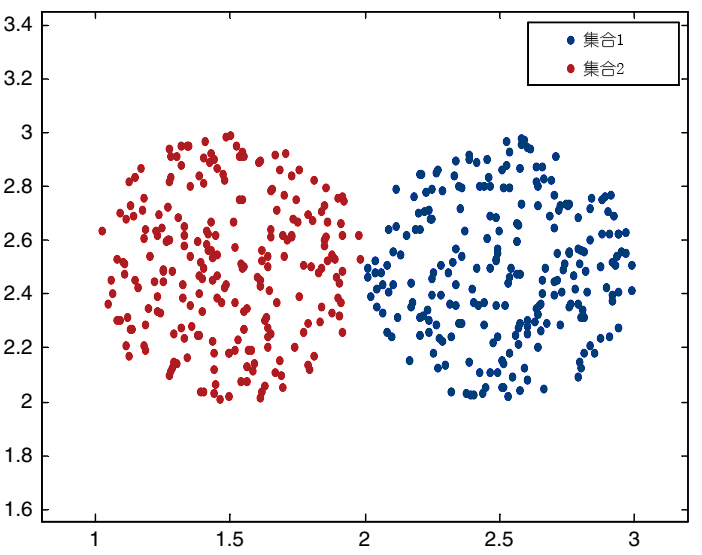
\includegraphics[width=\linewidth]{img/expr.png}
		\caption{测试数据集}
		\label{s4-img-f1}
	\end{minipage}%
	\hfill%
	\begin{minipage}[t]{0.3\linewidth}
		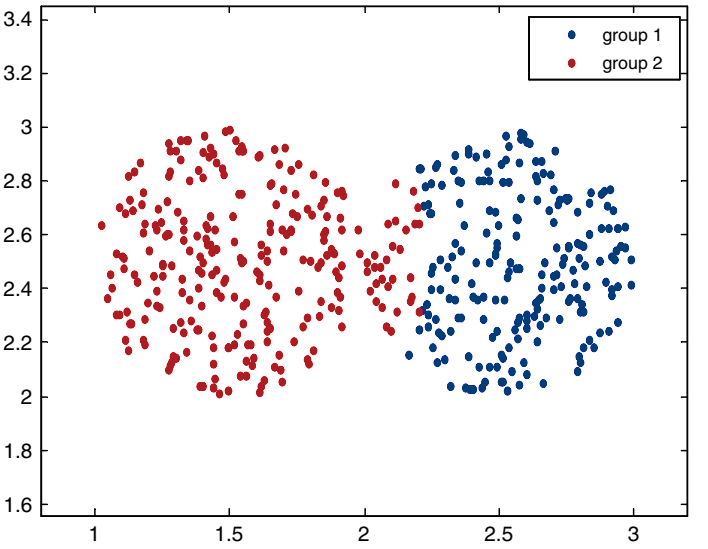
\includegraphics[width=\linewidth]{img/expr2.png}
		\caption{DBSCAN聚类结果}
		\label{s4-img-f2}
	\end{minipage}
	\hfill%
	\begin{minipage}[t]{0.3\linewidth}
		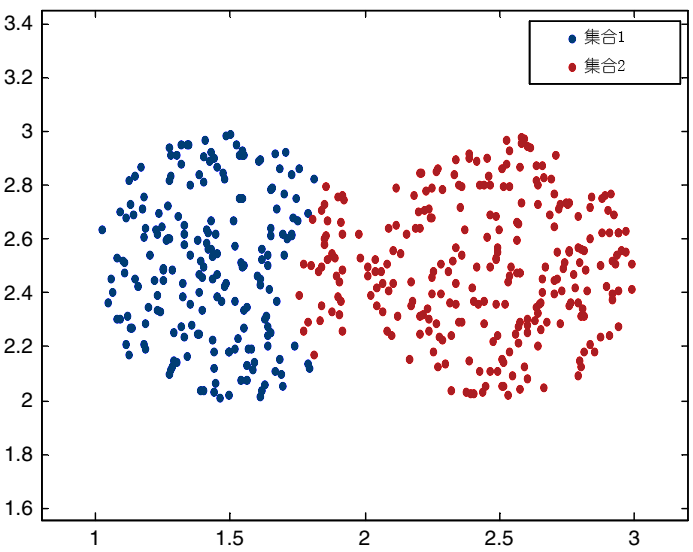
\includegraphics[width=\linewidth]{img/expr3.png}
		\caption{数据打乱后DBSCAN聚类结果}
		\label{s4-img-f3}
	\end{minipage}
\end{figure}

在论文\cite{tran2013revised}中,作者认为边界对象在传统DBSCAN算法中对簇的扩展没有贡献,因此可以通过改造算法的形式,以使得边界点的划分结果稳定。
文章提出在聚类过程中,暂时不处理边界对象,直到所有核心对象都被分配到对应的簇中。
最后,将所有未被划分的边界对象划分到最近的核心对象所属簇中即可。
在相同的数据集上,改进的DBSCAN算法划分结果如图\ref{s4-reDBSCANimg}所示:

\begin{figure}[htbp] %[htbp]
	\centering
	%	\captionsetup{font=scriptsize}
	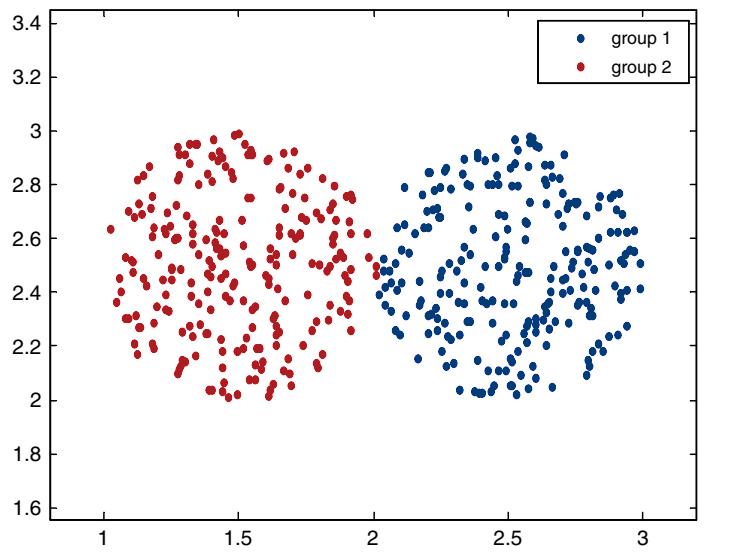
\includegraphics[scale=0.2]{img/expres.png}
	\caption{改进的DBSCAN算法划分结果}
	\label{s4-reDBSCANimg}
\end{figure}

\subsection{基于DBSCAN的层次聚类}
%先说问题
传统DBSCAN算法中,minPts和$ \epsilon $的取值对于聚类效果有极大影响,但同时又难以确定最合适的取值,因为二者受数据分布的影响较大。
同时,实际应用中数据大多不是均匀分布的,包含多个密度,若仅选择固定的一个$ \epsilon $值来进行聚类,难以获取全面的划分的结果。
适合高密度簇的$ \epsilon $值较小,能够对数据密集的区域进行较好的聚类,但是对于数据分布比较稀疏的簇聚类效果较差,可能会将较多数据划分为噪声。
因此,需要设置多个$ \epsilon $值来获取正确的聚类结果,这样的问题在高维数据集中比较常见。

%再说解决
为了解决上述问题,论文\cite{latifi2021dbhc}提出一种基于DBSCAN的层次聚类方案。
该算法的核心思想是,首先借助$ k $近邻算法和$ k $线图来获取多个$ \epsilon $值。
然后根据不同的$ \epsilon $值分别运行DBSCAN算法进行聚类,已经被聚类的内容不再参与后续聚类过程,直到遍历完所有$ \epsilon $值。
最后,若划分所得簇个数$ |C| $超过了用户实际需要的数量$ k $,则反复选择最近的簇进行合并,直到满足要求。

%最后说说参数
关于参数minPts、k以及$\epsilon$的获取依据论文已经详细给出,这里仅进行简单概况。minPts值越小,形成的簇个数越多,相反则越少。
如果minPts=1,则会创建密度为1的簇,不合理。若minPts=2,则DBSCAN的结果近似于层次聚类的结果,因此minPts的最小值应为3,最大值则是通过数据集大小$ M $和簇的个数$ C $给出,$ minPts_{max} = M\div C $。
经过分析,若minPts取值为3,则$ k $的取值为2,具体依据在论文\cite{latifi2021dbhc}的3.1节。
由于数据集中具体包含多少个不同的密度是无法获知的,因此采取用系列$\epsilon$值迭代聚类的策略来获取最终结果,$\epsilon$的取值主要借助$ k $线图获取。方法在算法\ref{alg_dbhc1}中给出:

\begin{algorithm}[htbp]
	\renewcommand{\algorithmicrequire}{\textbf{输入:}}
	\renewcommand{\algorithmicensure}{\textbf{输出:}}
	\caption{步骤一}
	\label{alg_dbhc1}
	\begin{algorithmic}[1]
		\REQUIRE 数据集$ D $
		\ENSURE $\epsilon$值集合$ E $
		\STATE $ m = |D| $
		\FOR{$ i=1 $ to $ m $}
		\STATE $ Dist[i] =$距离$i$第二近的距离
		\ENDFOR
		\STATE 以升序排列$ Dist $
		\STATE $ j = \sqrt{m} $
		\WHILE{$ j < m $}
		\STATE $ \{E\} = \{E\} + Dist[j] $
		\STATE $ j = j + \sqrt{m} $
		\ENDWHILE
	\end{algorithmic}
\end{algorithm}

首先,获取数据集的大小$ m $,在计算点之间的距离后,找到每个点第二近的距离。按照升序排列所有距离值$ Dist $,然后以$ \sqrt{m} $为间隔在$ Dist $中取值,即所需$\epsilon$值。

根据$ \epsilon $值获取划分初始簇的具体流程如算法\ref{alg_dbhc2}所示。
每次取最小的$\epsilon$值来执行DBSCAN,设置minPts的值为3。
然后,将本轮划分好的数据从原始数据集中剔除,不再参与后续聚类过程。
最后,将本轮迭代所用的$\epsilon$值剔除,重复上述过程,直到遍历完所有$\epsilon$值。
值得一提的是,这里没有被划分的点视为噪声,不会影响最终的聚类结果。
\begin{algorithm}[htbp]
	\renewcommand{\algorithmicrequire}{\textbf{输入:}}
	\renewcommand{\algorithmicensure}{\textbf{输出:}}
	\caption{步骤二}
	\label{alg_dbhc2}
	\begin{algorithmic}[1]
		\REQUIRE 数据集$ D $,$\epsilon$值集合$ E $
		\ENSURE 初始簇
		\WHILE{$ |E| > 0 $}
		\STATE $ e = \text{min}(\{E\}) $
		\STATE 执行DBSCAN(D, e, 3)
		\STATE $ D^{\prime} $为已经被划分所属簇的点
		\STATE $ \{D\} = \{D\} - D^{\prime} $
		\STATE $ \{E\} = \{E\} - e $
		\ENDWHILE
	\end{algorithmic}
\end{algorithm}

最后,将算法\ref{alg_dbhc2}中获取的初始簇进行合并获取最终结果。
如算法\ref{alg_dbhc3}所示,首先计算所有簇的中心,即累加簇中所有数据的值并取平均。
然后计算簇中心之间的距离,选择最近的两个簇合并,形成一个新的簇,重新计算簇中心,并且更新数据点的划分关系,将合并簇中所有数据的标识统一,初始簇集合大小减一。
重复上述过程,直到剩余簇个数为给出的$ k $个,即完成聚类。

\begin{algorithm}[htbp]
	\renewcommand{\algorithmicrequire}{\textbf{输入:}}
	\renewcommand{\algorithmicensure}{\textbf{输出:}}
	\caption{步骤三}
	\label{alg_dbhc3}
	\begin{algorithmic}[1]
		\REQUIRE 目标簇个数$ k $,初始簇
		\ENSURE 聚类结果
		\STATE 初始簇个数为$ n $
		\STATE 计算每个簇的中心
		\WHILE{$ n > k $}
		\STATE 找到最近的两个簇$ C $和$ C^{\prime} $
		\STATE 合并$ C $和$ C^{\prime} $
		\STATE 计算新簇的中心
		\STATE $ n = n-1 $
		\ENDWHILE
	\end{algorithmic}
\end{algorithm}
\section{问题描述}
\label{s4-wenti}
\subsection{系统模型}
如图\ref{s4-sysmod}所示,系统由两个部分组成:服务器端和用户端。与图\ref{sys model}类似,服务器端为两个云服务器,获取用户数据后执行一系列安全协议,最后分发结果。
\begin{figure}[htbp]
	\centering
	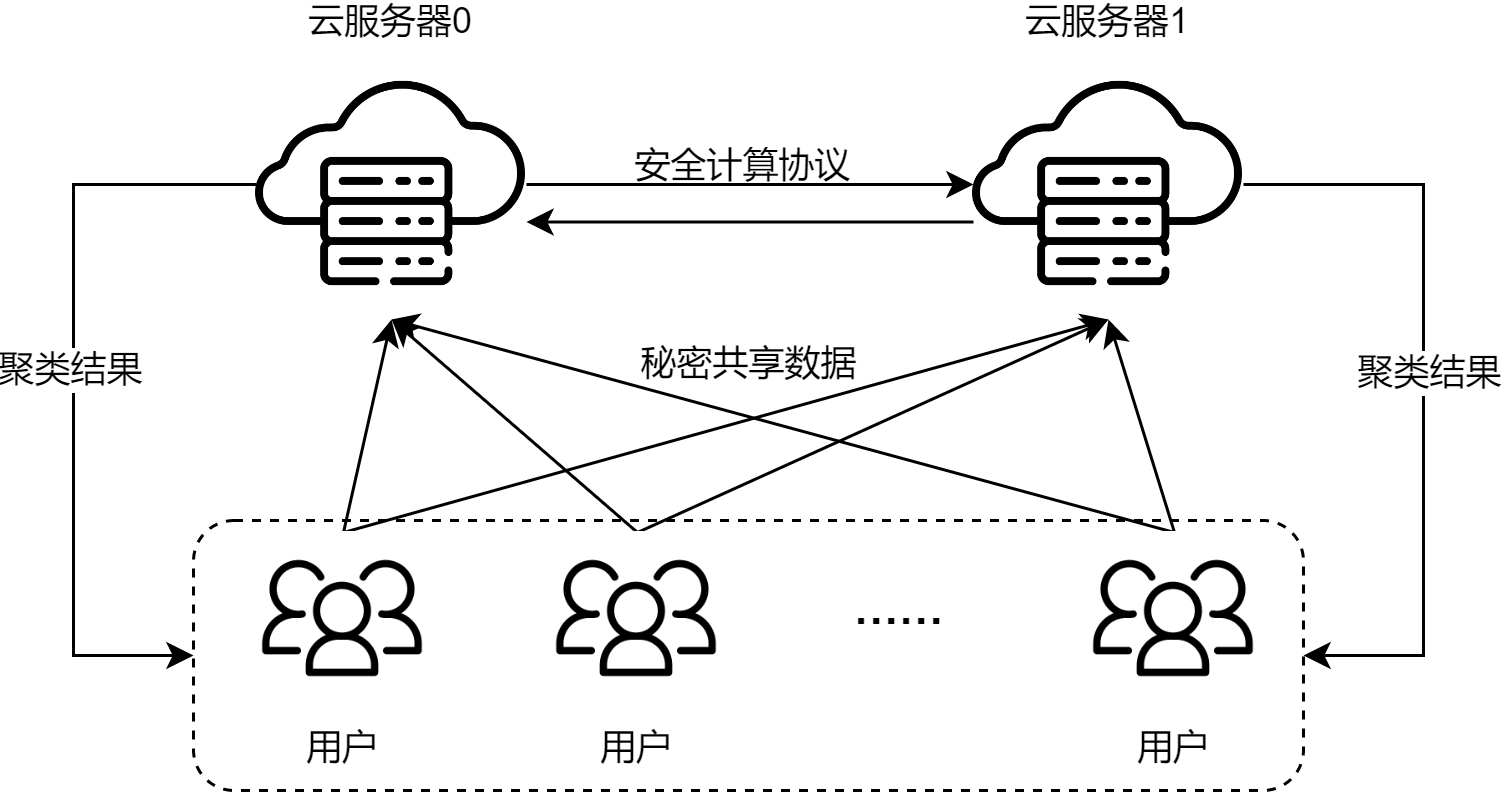
\includegraphics[width=0.7\linewidth]{img/sysmodel2.png}%width=\linewidth
	\caption{隐私保护DBSCAN方案系统模型}
	\label{s4-sysmod}
\end{figure}

不同的是,图\ref{sys model}中客户端为某一个持有全部明文数据的组织机构,本方案系统模型中的用户既可以是单一机构,也可以是各自持有不共享数据的不同机构。第二种场景下,用户可以是不同的医疗机构,期望能够在不泄露患者信息的情况,联合起来对医疗诊断或者症状信息进行聚类。用户各自将数据进行秘密共享后发送给双云服务器即可。在获取到聚类结果后,不同机构各自执行简单的算法来还原结果。


\subsection{安全模型}
本方案基于半诚实模型的假设,细节说明见\ref{s3-anquanmoxing}小节。具体而言:

对用户来说,持有数据的不同用户可能会根据聚类结果和云平台给予的信息,推断其他用户输入数据的具体内容。

对服务端来说,不共谋的云平台可能会试图根据秘密共享的数据、中间计算结果以及聚类结果推测原始内容,挖掘关键信息。
\subsection{设计目标}
针对三个解决不同问题的隐私保护DBSCAN方案,设计目标不尽相同。对于方案一,本文期望
\begin{compactitem}
	\item\textbf{高效性:}遵循明文DBSCAN算法的思路,设计一个效率较高的密文方案,使得通信和计算开销均较小。与前沿隐私保护DBSCAN方案相比,在不损失安全性的前提下更加高效。
	\item\textbf{准确性:}我们的首要目标是密文方案与明文方案聚类结果一致,设计可靠的安全计算协议,获取精度不受损失的聚类划分结果。
	\item\textbf{安全性:}我们重点关注如何在密度聚类的过程中,保护用户原始数据、中间计算结果和最终聚类结果中包含的隐私或敏感信息,防止云服务器或其他用户获取相关信息。
	%	用于聚类的原始数据、中间计算结果以及最终的聚类划分结果均不会被泄露。半诚实模型下的云平台能够遵循协议的执行,但无法从计算过程中推断出任何有用信息。
\end{compactitem}

在上述目标的基础上,方案二的设计目标为,在效率损失可接受的情况下,设计一个能够获取稳定聚类划分结果的隐私保护DBSCAN方案,在方案一的基础上提升聚类结果的质量,不损失任何安全性。

方案三的设计目标为,设计一个能够不依赖人工设置参数的隐私保护DBSCAN方案,方案能够有效划分包含不同密度数据的数据集,同时无需对数据集进行前置数据分析以获取适合的$\epsilon$和minPts值,最后获得近似的划分结果。

\subsection{系统输入}
数据持有者首先利用加性秘密共享来将数据划分为两份,分别发送给两个云服务器。采用加性秘密共享分发数据的方式允许系统中加入任意多个数据持有者提供聚类数据。此外,本文所述系统能够支持任何数据划分方式,例如水平划分、垂直划分以及混合划分。水平划分方式指的是,不同用户分别持有完整但是互异的数据\cite{gheid2016efficient},垂直划分方式则是指不同用户持有相同数据记录的不同参数\cite{doganay2008distributed},混合划分方式则是上述两种方式的结合\cite{yu2010multi}。
\section{基于秘密共享的隐私保护计算模块}
\label{s4-subpro}
在\ref{s3-mokuai}节所述安全计算协议的基础上,根据隐私保护DBSCAN方案的特点设计了如下计算模块。
\subsection{安全排序协议}
安全排序协议主要由安全比较协议构成,用户输入秘密共享的数组后,期望能够得到按照升序排列的密文结果。协议的核心思想为,将$ n $个数据上的排序拆分为$ n $次求解序列最值。

具体过程如算法\ref{alg_sort}所示,进行$ n $次迭代,首先求解最小值,结果为秘密共享值$ \langle t_i \rangle \in \{0,1\}, i\in[1,n] $,数组中最小值的位置为1,其余均为0。
然后,开始遍历每个结果,$ res $通过累加记录最小值的具体值,并更新原始数组,通过将最小值变为最大值max,以消除对后续计算的影响。
若当前元素为最小值(即$\langle t_i \rangle=1  $ ),则对应$ D[i] $中的值变为max,若不是则保留原值,不做修改。最后,将累加获得最小值$ res $存放到$ D^{\prime}[i] $中以获得升序排列的结果。

\begin{algorithm}[htbp]
	\renewcommand{\algorithmicrequire}{\textbf{输入:}}
	\renewcommand{\algorithmicensure}{\textbf{输出:}}
	\caption{安全排序协议}
	\label{alg_sort}
	\begin{algorithmic}[1]
		\REQUIRE $ D \leftarrow \{\langle  x_1 \rangle, \langle  x_2 \rangle,...,\langle  x_n \rangle\} $
		\ENSURE 排序结果 $ D^{\prime} \leftarrow \{\langle  x^{\prime}_1 \rangle, \langle  x^{\prime}_2 \rangle,...,\langle  x^{\prime}_n \rangle\} $
		\FOR{$ i=1 $ to $ n $}
		\STATE $ \{\langle  t_1 \rangle,...\langle  t_n \rangle\} \leftarrow \text{SMin}(D)$
		\STATE $ res \leftarrow 0 $
		\FOR {$ j=1 $ to $ n $}
		\STATE $ res \leftarrow res + \text{MUL}(\langle  t_j \rangle, D[j]) $
		\STATE $ D[j] \leftarrow \text{MUL}(D[j],1-\langle  t_j \rangle) + \text{MUL}(\text{max}, \langle  t_j \rangle)$
		\ENDFOR
		\STATE $ D^{\prime}[i] \leftarrow res $
		\ENDFOR
	\end{algorithmic}
\end{algorithm}
\section{隐私保护DBSCAN方案}
\label{s4-t1}
在正式介绍本文设计的隐私保护DBSCAN方案之前,首先通过一个示例来详细阐述方案的核心思想。在DBSCAN算法的基础上,本文引入了临时簇的概念,令核心对象与其$ \epsilon $范围内未被划分的边界对象组成独立的临时簇,临时簇内所有数据对象的簇标识保持一致。
在遍历的过程中对于核心对象,修改其$ \epsilon $范围内未被划分的边界对象的簇标识,与当前核心对象保持一致。对于核心对象$ \epsilon $范围内的其他核心对象,记录二者的相邻关系。
在还原聚类结果时,根据临时簇之间的相邻关系构造邻接矩阵(相邻对象在矩阵中对应值大于0),通过深度优先遍历算法找到相邻的临时簇合并,不相邻的临时簇不受影响。

\begin{figure}[htbp]
	\begin{minipage}[t]{0.48\linewidth}
		\centering
		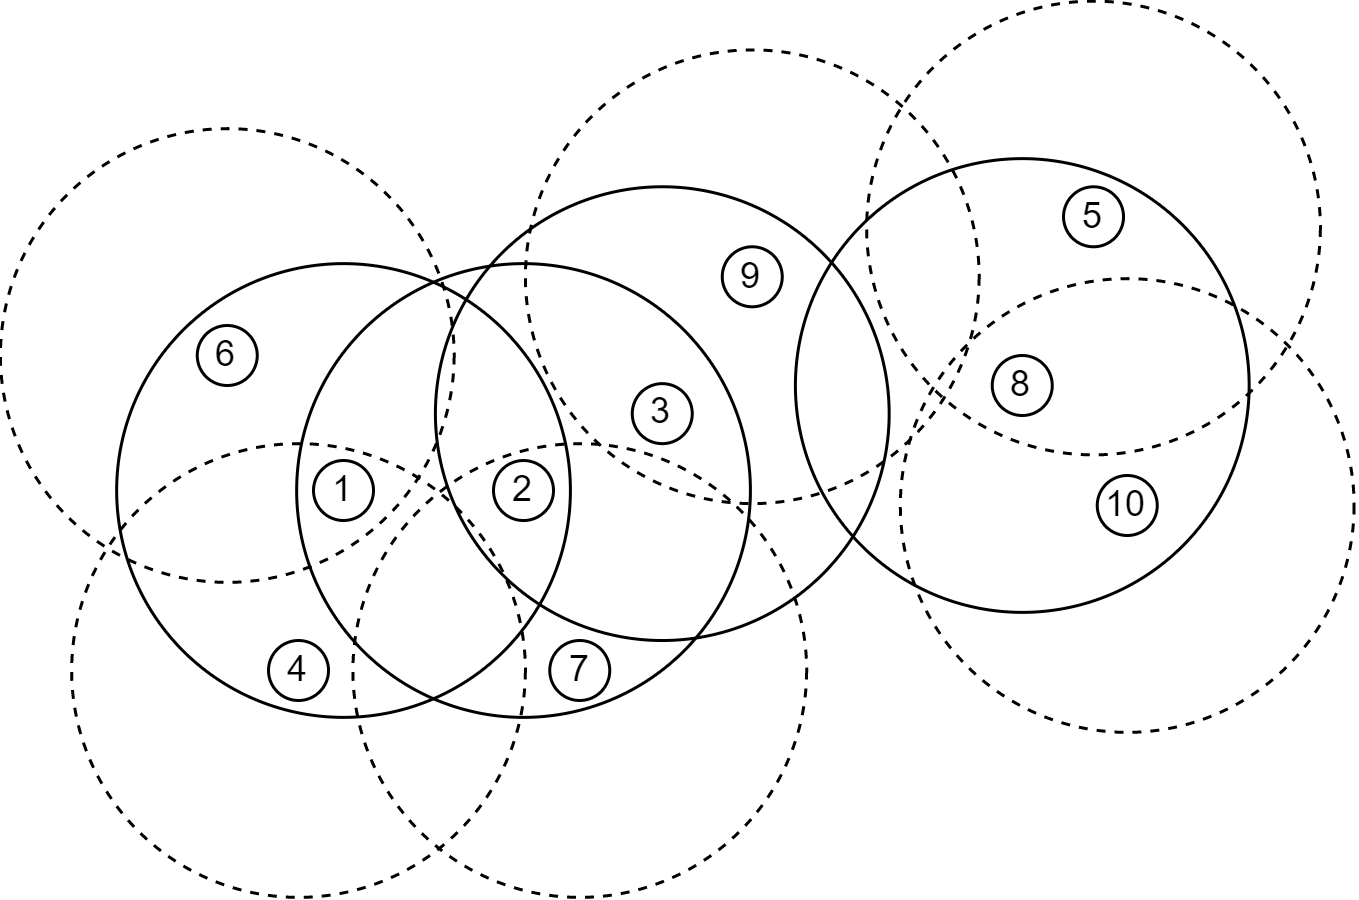
\includegraphics[width=\linewidth]{img/dbraw.png}
		\caption{示例数据可视化}
		\label{dataraw}
	\end{minipage}
	\hfill
	\begin{minipage}[t]{0.48\linewidth}
		\centering
		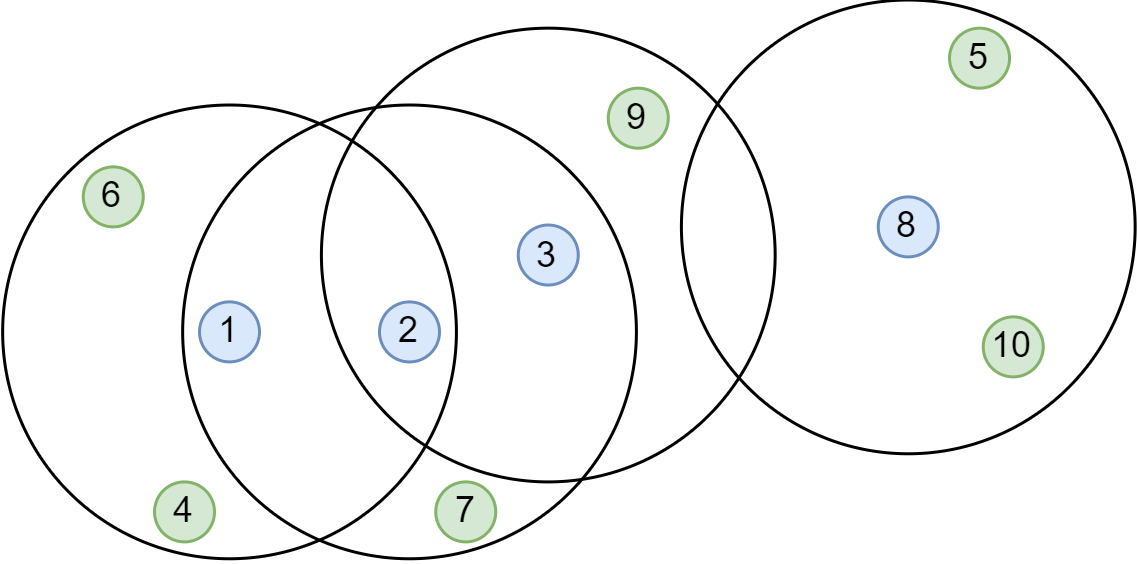
\includegraphics[width=\linewidth]{img/db1.png}
		\caption{核心对象与边界对象}
		\label{dbraw}
	\end{minipage}
\end{figure}

假设当前有一个包含10个点的数据集$ \{p_1,...,p_{10}\} $,令minPts为2,用圆圈框出所有数据对象的$ \epsilon $邻域,数据集可视化后如图\ref{dataraw}所示,其中虚线框为边界对象$ \epsilon $邻域,实线框为核心对象$ \epsilon $邻域。
在图\ref{dbraw}中,我们用蓝色表示核心对象,绿色表示边界对象,噪声点在聚类过程中不会进行任何处理,为了简化表示,示例数据集没有噪声点。

接下来,在上述示例数据集的基础上,将详细介绍聚类的过程。下述过程按照编号$ \{1,2,...,10\} $进行遍历,每一个数据对象的初始簇标识为图中序号。首先,对$ p_1 $进行处理,在其$ \epsilon $范围内,有边界对象$ p_6$、$p_4 $和核心对象$ p_2 $。针对边界对象,我们修改其编号与$ p_1 $保持一致;针对核心对象,我们记录相邻关系;不在$ \epsilon $范围内的点(例如$ p_3 $和$ p_9 $),不做任何处理。对$ p_1 $遍历完所有数据对象后,结果如图\ref{db_one}所示。

\begin{figure}[htbp]
	\centering
	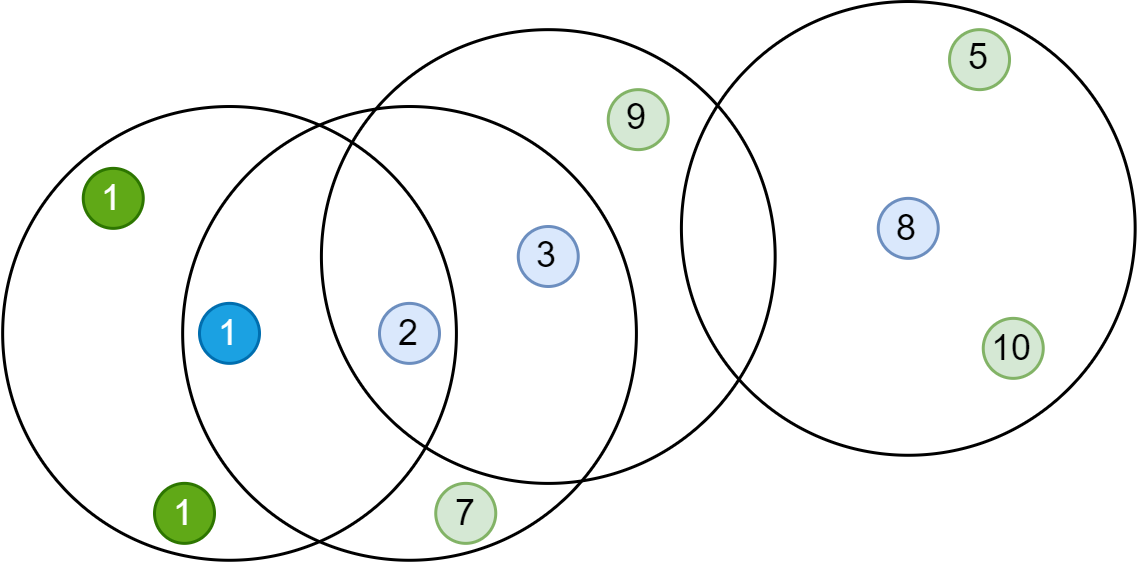
\includegraphics[width=0.6\textwidth]{img/db2.png}
	\caption{$ p_1 $处理结果}
	\label{db_one}
\end{figure}

其他核心对象($ p_2 $、$ p_3 $和$ p_8 $)的处理和$ p_1 $一致(详细过程见图\ref{db_process}中的a、b和c),每一步进行处理的数据对象均将颜色加深,可以看到已经处理过的核心对象和边界对象的cluId不会受到任何影响,核心对象之间仅记录连接关系。处理核心对象$ p_8 $时,范围内没有任何其他核心对象,因此不会记录任何连接关系。同时,当遍历到边界对象时,不会记录和修改任何信息。

\begin{figure}[htbp]
	\centering
	\subfloat[$ p_2 $处理结果]{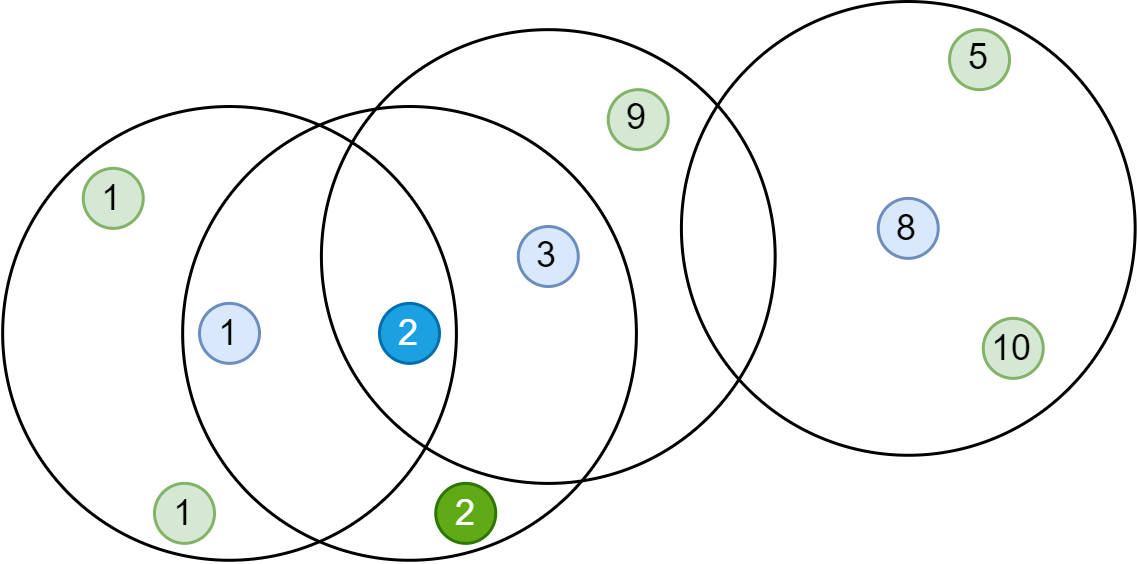
\includegraphics[width=0.29\textwidth]{img/db3.png}}
	\subfloat[$ p_3 $处理结果]{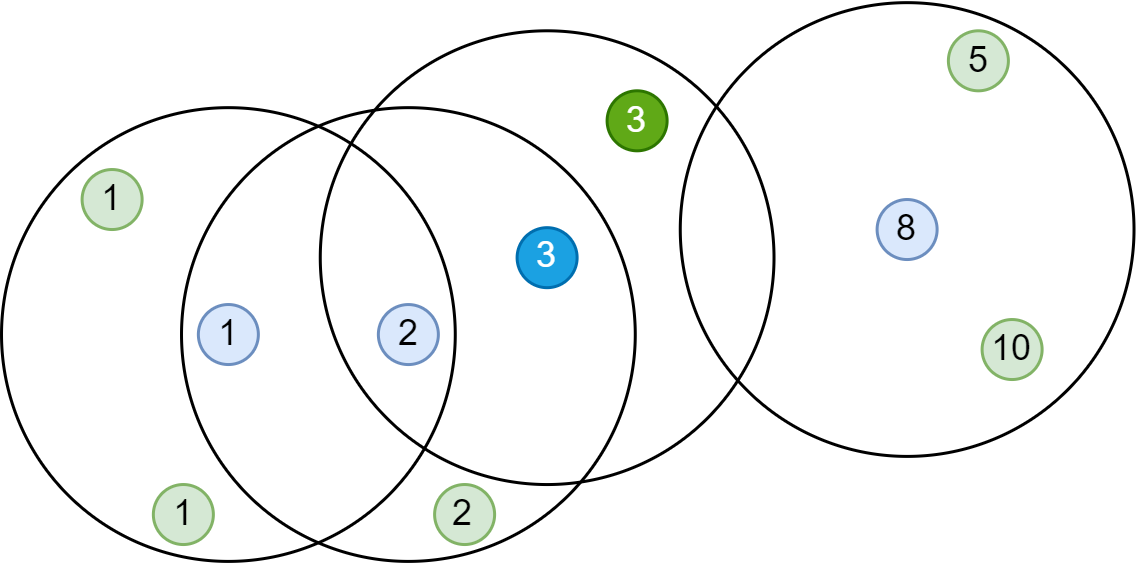
\includegraphics[width=0.29\textwidth]{img/db4.png}}
	\subfloat[$ p_8 $处理结果]{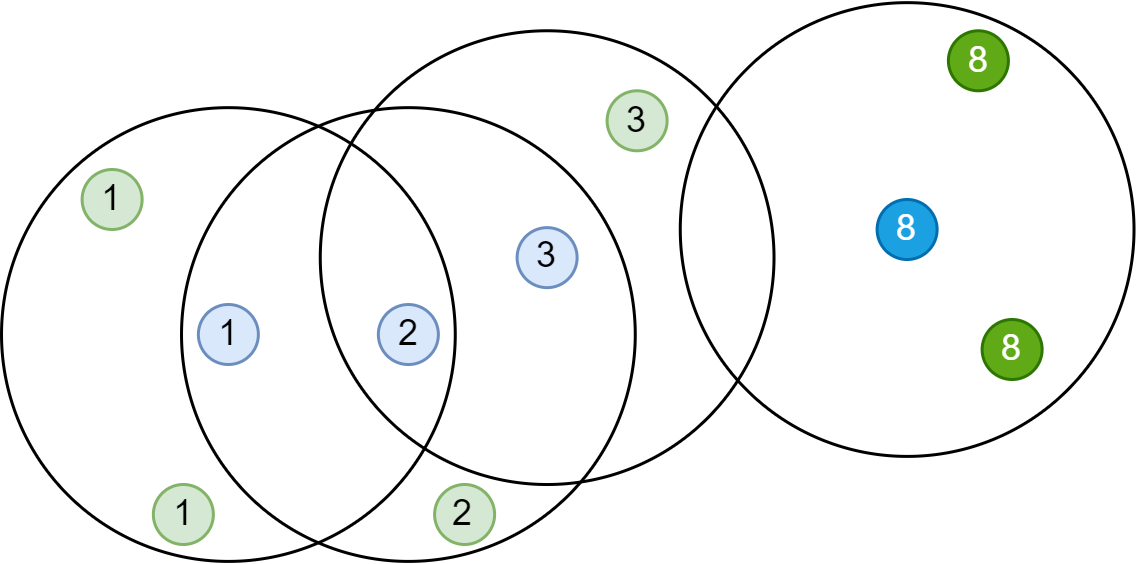
\includegraphics[width=0.29\textwidth]{img/db5.png}}
	\caption{聚类处理过程}
	\label{db_process}
\end{figure}

接下来,我们根据遍历过程中存储的相邻关系构造矩阵,结果如图\ref{db_matrix}所示,可以看到只有核心点之间存在相连关系(灰色部分)。基于该邻接矩阵,运行深度优先遍历算法,可以将cluId为1、2和3的临时簇进行合并。

\begin{figure}[htbp]
	\centering
	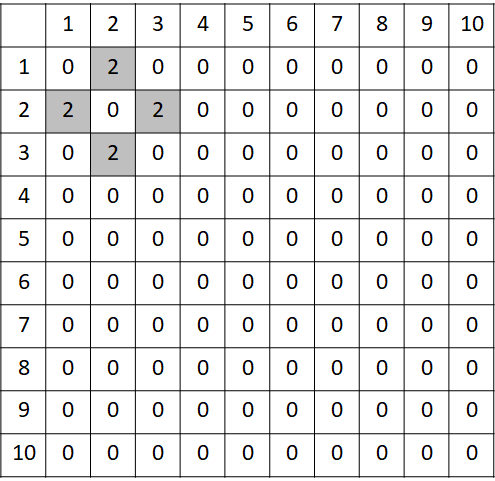
\includegraphics[width=0.4\textwidth]{img/db_matrix.png}
	\caption{临时簇相连关系}
	\label{db_matrix}
\end{figure}

经过合并后,得到最终聚类结果,如图\ref{dbres}所示,可以看到数据集包含两个簇,其中黄色对象被划分到簇1中,紫色对象被划分到簇2中。
\begin{figure}[htbp]
	\centering
	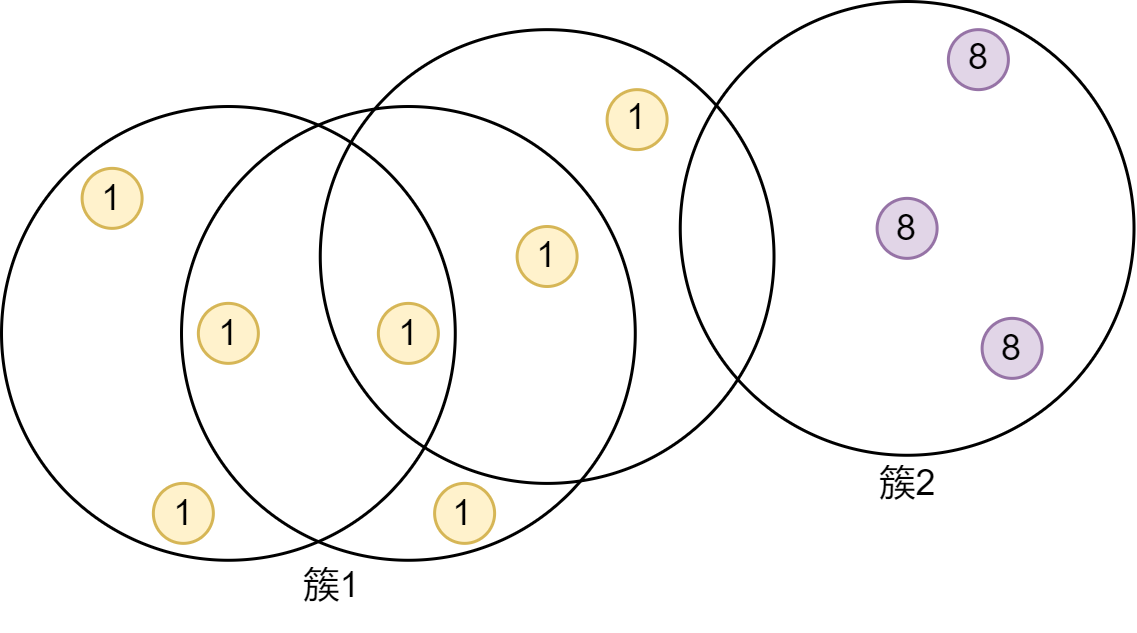
\includegraphics[width=0.6\textwidth]{img/dbres.png}
	\caption{还原聚类结果}
	\label{dbres}
\end{figure}

以上即是本节所述密文方案的具体示例,方案的复杂度为$ O(n^2) $,与明文方案一致。我们通过限制临时簇只能包含未被划分的边界对象,以避免边界对象被反复划分到不同的临时簇中的问题。

明文DBSCAN算法采取的策略是随机选择一个未被划分的核心对象,不断的找到密度可达的其他核心对象并将所有相邻的边界对象纳入当前簇集合,直到没有新的核心对象能加入当前簇集合。
若沿用上述思路直接设计密文方案,会导致方案复杂度达到$ O(n!) $,计算开销过大难以应用于实际场景中。
因此本文引入临时簇的概念,将方案的迭代深度减少为2,极大的降低了密文方案的复杂度。
记录相连关系本质上是在记录核心对象之间的密度可达关系,密度不可达的核心对象以及边界对象在邻接矩阵中的值都为0。
最后我们让用户在明文上基于相邻关系运行深度优先遍历将相邻的临时簇进行合并,来获取最终聚类结果。各自持有数据的独立用户,无法知道彼此拥有的明文数据,仅知道簇的划分情况,达到了保护数据安全的目的。

接下来详细介绍本文提出的隐私保护DBSCAN方案的具体过程,主要分为三个阶段,具体介绍如下:
\begin{compactitem}
	\item \textbf{预处理元素:}通过获取的密文数据,初始化存储在云服务器上的自定义数据结构体(以下简称元素),然后计算不同元素之间的欧式距离关系,并判断每个元素是否为核心点。
	\item \textbf{密度聚类:}根据第一阶段获取的信息,提出了一种全新的聚类方法,引入临时簇这一概念,结合不同核心对象之间的相连关系,可以将相连的临时簇进行合并。聚类过程即是标记临时簇,并记录相连信息。
	\item \textbf{还原聚类结果:}用户获取聚类记录的临时簇相连信息和簇标记信息,通过深度优先遍历算法来还原数据簇划分结果。
\end{compactitem}

\subsection{预处理元素}
% 首先介绍input element
云平台分别获取用户密文数据后,初始化聚类所需元素。基于每个秘密共享的数据sdata分别构造sharedElem对象,sharedElem内的所有值均为秘密共享值,详细结构如算法\ref{s4-sharedelem}所示。
cluId,cluId $ \in [1, n]$为初始簇中心,值取该数据在数组中的顺序,比如第一个数据初始化cluId为1,最后一个数据的cluId则为n。
isMark,isMark$ \in [0,1] $表示该数据对象是否已经被划分到簇中,0表示未被划分到簇中,1则表示已经被划分,初始化为0。
data则存储该数据对应的秘密共享值sdata,是一个大小为$ m $的向量,主要用于计算数据点之间的欧式距离。
isCore,isCore$ \in[0,1]$标识数据对象是否为核心点,主要用于在聚类时参与计算,初始化为0,即默认非核心点。
resCId记录最终划分结果,在用户还原结果时使用,初始化为0值。


\begin{algorithm}
	\caption{sharedElem数据结构}
	\label{s4-sharedelem}
	\begin{algorithmic}[1]
		\STATE \textbf{class} sharedElem(sdata,idx):
		\STATE \hspace{\algorithmicindent} cluId = idx
		\STATE \hspace{\algorithmicindent} isMark = 0
		\STATE \hspace{\algorithmicindent} data = sdata
		\STATE \hspace{\algorithmicindent} isCore = 0
		\STATE \hspace{\algorithmicindent} resCId = 0
	\end{algorithmic}
\end{algorithm}

构造完sharedElem对象后,得到了长度为$ n $的sharedList数组。
在初始化阶段,我需要们计算对象之间的距离,获取相邻关系,同时判断每个元素是否为核心点。
具体过程如算法\ref{alg_t1_s1}所示。
首先,构造数组cnt存储每个元素$ \epsilon $邻域范围内包含其他元素的个数。
然后,通过DIST计算元素之间的欧式距离,去掉根号便于计算,将第$ i $个元素与其他所有元素的距离$ d[j],j\in[n] $与$ \epsilon $进行一次安全比较,判断二者是否相邻,结果存储到二维数组$ u[i][j],i,j\in[n] $中,最后累加$ u[i][j],j\in[n]$的值,统计元素$ i $邻域范围内包含点的个数,存储到cnt中。
最后,并行比较存储邻域点个数的cnt数组与长度为$ n $的值均为minPts的数组之间的大小关系,并更新sharedList的isCore属性。

\begin{algorithm}[htbp]
	\renewcommand{\algorithmicrequire}{\textbf{输入:}}
	\renewcommand{\algorithmicensure}{\textbf{输出:}}
	\caption{预处理元素}
	\label{alg_t1_s1}
	\begin{algorithmic}[1]
		\REQUIRE 数组sharedList简写为$ \{x[1],...,x[n]\} $
		\ENSURE 相邻关系二维数组$ u $,更新后的$ x $
		\STATE $ cnt \leftarrow [0,...,0]_n $
		\FOR {$ i=1 $ to $ n $}
		\FOR {$ j=1 $ to $ n $}
		\STATE $ d[j] \leftarrow \text{DIST}(x[i].data, x[j].data) $
		\ENDFOR
		\STATE $ u[i] \leftarrow \text{SC}(d, [\epsilon,...,\epsilon]_n) $
		\STATE $ cnt[i] \leftarrow \text{sum}(u[i][j])$ for $j \in [n] $
		\ENDFOR
		\STATE $ r \leftarrow \text{SC}([minPts,...]_n,cnt) $
		\FOR {$ i=1 $ to $ n $}
		\STATE x[i].isCore = r[i]
		\ENDFOR
	\end{algorithmic}
\end{algorithm}

值得一提的是,这里的$\epsilon$值与明文DBSCAN算法中的不同,对欧式距离计算舍去根号,因此$\epsilon$值在原来的基础上取平方,为了方便表示,这里省略了详细说明。minPts的值则不做任何修改,在后面的实验分析中,本文会根据上述改动提供修改后的$ \epsilon $值。


\subsection{密度聚类}
\label{t1-julei}
初始化之后,获得了元素的isCore信息,以及元素之间的相邻关系$ u[i][j] \in \{0,1\},i,j\in[n]$。接下来,这里将详细说明如何根据预处理过程中已经获取的信息进行聚类。

在本节的开头提到了基于DBSCAN设计隐私保护聚类方案的难点,论文\cite{bozdemir2021privacy}为了解决这个问题,提出了两种解决办法,一方面可以人工设置最大迭代深度,但是该方法不具备普适性,每次都需要结合数据集的特点给出最大迭代深度;另一方面则是通过还原1比特的数据来判断是否需要终止迭代。
本文为了解决这一问题,引入了临时簇,在遍历过程中,记录临时簇之间的相连关系(即核心对象之间的距离小于$\epsilon$),同时核心对象会将邻域范围内所有未被标记的边界对象的cluId修改为与自身一致。在获取聚类结果阶段,构造邻接矩阵,将相连的临时簇进行合并,获取划分结果。
相连信息存储在info数据结构中,具体内容如算法\ref{s4-info}所示,其中id1和id2记录sharedElem中的cluId信息,isConn则记录临时簇之间的相连关系,取值为0或1。
\begin{algorithm}
	\caption{info数据结构}
	\label{s4-info}
	\begin{algorithmic}[1]
		\STATE \textbf{class} info(cluId1, cluId2, isConn):
		\STATE \hspace{\algorithmicindent} id1 = cluId1
		\STATE \hspace{\algorithmicindent} id2 = cluId2
		\STATE \hspace{\algorithmicindent} conn = isConn
	\end{algorithmic}
\end{algorithm}

在初始化的过程中,默认每个元素的初始cluId为下标$ \{1,2,...,n\} $。在聚类的过程中,对于核心对象,修改其$ \epsilon $范围内所有未被标记的边界对象的cluId,并将状态修改为已标记。对于所有非核心点,无法修改其他点的属性,并且被标记后,无法再被其他核心点标记,噪声不会受到任何影响。经过上述过程,数据集已经被划分为若干临时簇,同一临时簇内所有数据对象的簇标识cluId一致。具体流程如算法\ref{alg_t1_s2}所示,为了简化说明,将输入数组sharedList简写为$ x $,并将相连关系的结果记录在plist数组中作为输出结果,每个元素的结构为info类型。
\begin{algorithm}[htbp]
	\renewcommand{\algorithmicrequire}{\textbf{输入:}}
	\renewcommand{\algorithmicensure}{\textbf{输出:}}
	\caption{密度聚类}
	\label{alg_t1_s2}
	\begin{algorithmic}[1]
		\REQUIRE 数组sharedList简写为$ x $,相邻关系$ u[i][j],i,j\in[n] $
		\ENSURE 簇连接关系$ plist $
		\FOR{$ i=1 $ to $ n $}
		\FOR {$ j=1 $ to $ n $,$ j\neq i $}
		\STATE $ m_1 \leftarrow \text{MUL}(x[i].isCore, u[i][j], 1-x[j].isCore) $
		\STATE $ m_2 \leftarrow \text{MUL}(m_1, 1-x[j].isMark) $
		\STATE $ x[j].cluId \leftarrow  \text{MUL}(m_2, x[i].cluId) + \text{MUL}(1-m_2, x[j].cluId)$
		\STATE $ conn \leftarrow \text{MUL}(x[i].isCore, x[j].isCore, u[i][j]) $
		\STATE 添加新元素 $ [x[i].cluId, x[j].cluId, conn] $ 到plist中
		\STATE $ x[j].isMark \leftarrow m_1 + x[j].isMark - \text{MUL}(m_1, x[j].isMark) $
		\ENDFOR
		\ENDFOR
	\end{algorithmic}
\end{algorithm}

在整个算法的执行过程中,通过各种运算来实现逻辑与和逻辑或,借助计算一些辅助标识来控制是否修改内容。
首先,获取标识$ m_1 $来辅助后续计算,若x[i]为核心对象、x[j]为非核心对象并且二者相邻,则$ m_1 $为1,否则为0。
若在$ m_1 $为1的情况下,x[j]未被标记,则$ m_2 $为1。这里根据$ m_2 $来控制是否修改x[j]的cluId,若不满足条件,则x[j]的cluId保持原样,否则修改为与x[i]的cluId一致。
conn反映的是x[i]与x[j]是否相连,若x[i]和x[j]均为核心对象并且相邻$ u[i][j]=1 $则conn等于1,否则为0,然后新增info类型的数据到plist中。值得一提的是,这里无论是否相邻,都会记录新的info信息,因此最终plist的长度为$ n(n-1) $。
最后,更新x[j]的isMark标识,若x[j]已被划分(isMark=1)或者本次迭代过程中应被划分($ m_1 = 1 $),则x[j]的isMark标识为1,否则为0。算法中的计算方式体现的是逻辑或关系。
论文\cite{bozdemir2021privacy}中提出的ppDBSCAN方案将复杂度从$ O(n^3)$降为$ O(maxIterations \cdot n^2) $,本节中,上述聚类过程的复杂度为$ O(n^2) $,并且不会产生任何精度损失也不会泄露任何密文信息,方案更加安全高效。

\subsection{还原聚类结果}
\label{task1-huanyuan}
聚类后,在plist中记录了所有临时簇的相邻关系,云服务器分别将自己持有的秘密共享信息发送给用户。用户运行$ \text{Rec}(\cdot,\cdot) $还原结果后获取相邻关系和cluId,在本地分别运行还原结果算法以获取最终结果。具体过程如算法\ref{alg_t1_s3}所示。
%在算法\ref{alg_t1_s3}和算法\ref{alg_t1_s4}中将详细说明如何还原结果。

\begin{algorithm}[htbp]
	\renewcommand{\algorithmicrequire}{\textbf{输入:}}
	\renewcommand{\algorithmicensure}{\textbf{输出:}}
	\caption{还原结果}
	\label{alg_t1_s3}
	\begin{algorithmic}[1]
		\REQUIRE 明文plist
		\ENSURE 获取resCId的plist
		\STATE 构造二维数组matrix,大小为$ n\times n $存储相连关系
		\STATE 构建resmap存储初始簇id到结果簇id的映射
		\FOR {each p in plist}
		\STATE matrix[p.id1][p.id2] += p.isConn
		\ENDFOR
		\STATE 构造访问标识数组$ visited=[false]_n $
		\STATE mark = 1
		\FOR {$ i=1 $ to $ n $}
		\IF{visited[i]为真}
		\STATE 不再继续访问
		\ENDIF
		\STATE visited[i] = true
		\STATE mark += 1
		\STATE resmap[plist[i].cluId] = mark
		\STATE 执行DFS(i, mark, visited, plist,matrix, resmap)
		\ENDFOR
		\FOR{$i=1$ to $n$}
		\IF{x[i].cluId in resmap}
		\STATE x[i].resCId $\leftarrow$ resmap[x[i].cluId]
		\ENDIF
		\ENDFOR
	\end{algorithmic}
\end{algorithm}

首先,构造大小为$ n \times n $的全零邻接矩阵,来存储邻接关系。
根据plist信息来还原相连信息,若相邻则邻接矩阵中,对应位置的值大于0。
然后,初始化一个数组visited来标记每个数据是否已经被划分到最终所属簇中,若已经被划分,则不再继续处理,这里用mark表示最终结果的簇编号,自1开始累加。
随后,开始遍历,若第$ i $个元素已被划分,则跳出当前循环,开始下一次。
若未被划分,则更新mark值自增1,然后开始构建新簇,从当前元素$ i $开始执行深度优先遍历找到所有与$ i $相连的元素纳入到新簇中。
找到所有相邻临时簇的过程如算法\ref{alg_t1_s4}所示,边递归边记录映射关系,将相连的临时簇进行合并。
最后,根据resmap映射关系,更新所有元素的最终簇编号resCId,这一步操作可以将属于同一个簇的所有临时簇中的数据点的cluId修改一致。

\begin{algorithm}[htbp]
	\renewcommand{\algorithmicrequire}{\textbf{输入:}}
	\renewcommand{\algorithmicensure}{\textbf{输出:}}
	\caption{深度优先遍历}
	\label{alg_t1_s4}
	\begin{algorithmic}[1]
		\REQUIRE 起始位置idx,归属簇标识mark,访问标识数组visited,元素数组plist,二维矩阵matrix,映射关系resmap
		\ENSURE 修改后的输入值
		\FOR {$ i=1 $ to $ n $}
		\IF {visited[i]为真}
		\STATE 该元素已经被划分好,不再继续
		\ENDIF
		\IF{matrix[idx][i] > 0}
		\STATE resmap[plist[i].cluId] = mark
		\STATE visited[i]=true
		\STATE DFS(i, mark, visited, plist,matrix, resmap)
		\ENDIF
		\ENDFOR
	\end{algorithmic}
\end{algorithm}

深度优先算法在这里应用的目的是将相连的临时簇合并成一个整体,从而获取最终的结果。在遍历的过程中,若判断相连,则建立该数据cluId到最终结果mark的映射关系,并存储到resmap中。

上述过程由用户独立运行,这里算法的复杂度最大为$ O(n^2) $,但是可以通过一些改进方法将深度优先遍历算法的复杂度降低为$ O(n) $,对用户来说,执行上述算法的开销较小。并且,云服务器返回聚类结果时其中sharedElem中的data、isCore以及isMark信息均不对用户揭露。

\section{改进的隐私保护DBSCAN}
\label{s4-t2}
本节将在上一节的基础上详细阐述一种改进的隐私保护DBSCAN方案,该方案能够在数据集被打乱的情况下,使满足可以被划分到多个簇条件的数据点获取稳定的划分结果,只需要在方案一的基础上引入一些比较和计算操作,即可提升聚类质量。

在前一章\ref{s4-t1}可视化示例的基础上,我们简述方案一和方案二的主要差异。初始数据集如图\ref{redata1}所示,然后开始遍历,仅处理非核心对象,这里没有噪声点,因此将所有边界对象的簇标识cluId都改成与最近的核心对象一致,核心对象不做任何修改,结果如图\ref{redata2}所示,所有边界对象均修改了簇标识(深绿色点)。对于噪声点,是否修改cluId都对最终结果没有任何影响。

\begin{figure}[!h]
	\begin{minipage}[t]{0.48\linewidth}
		\centering
		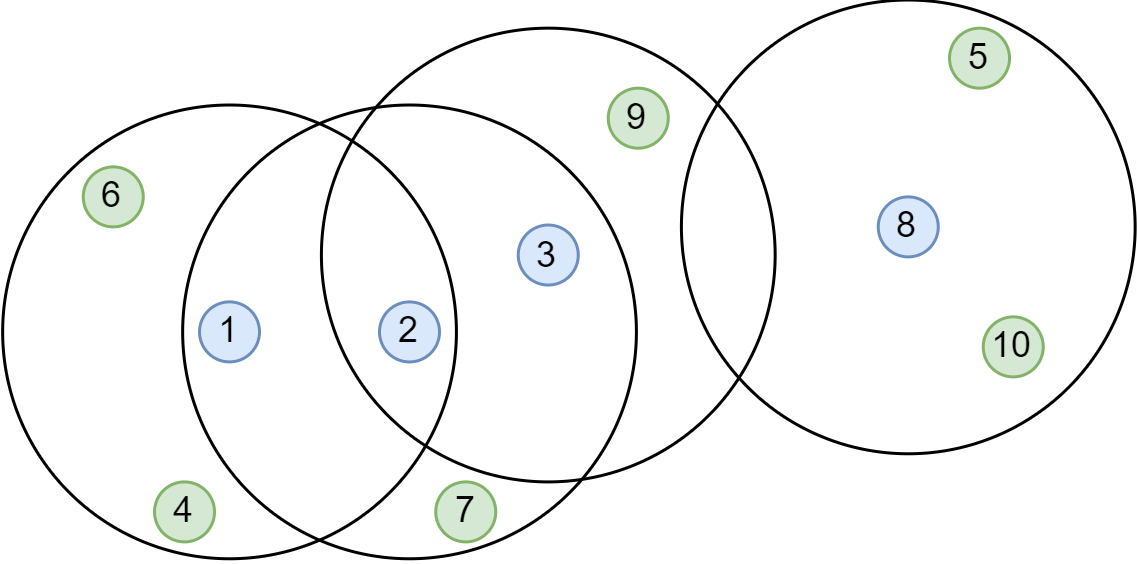
\includegraphics[width=\linewidth]{img/db1.png}
		\caption{初始数据集}
		\label{redata1}
	\end{minipage}
	\hfill
	\begin{minipage}[t]{0.48\linewidth}
		\centering
		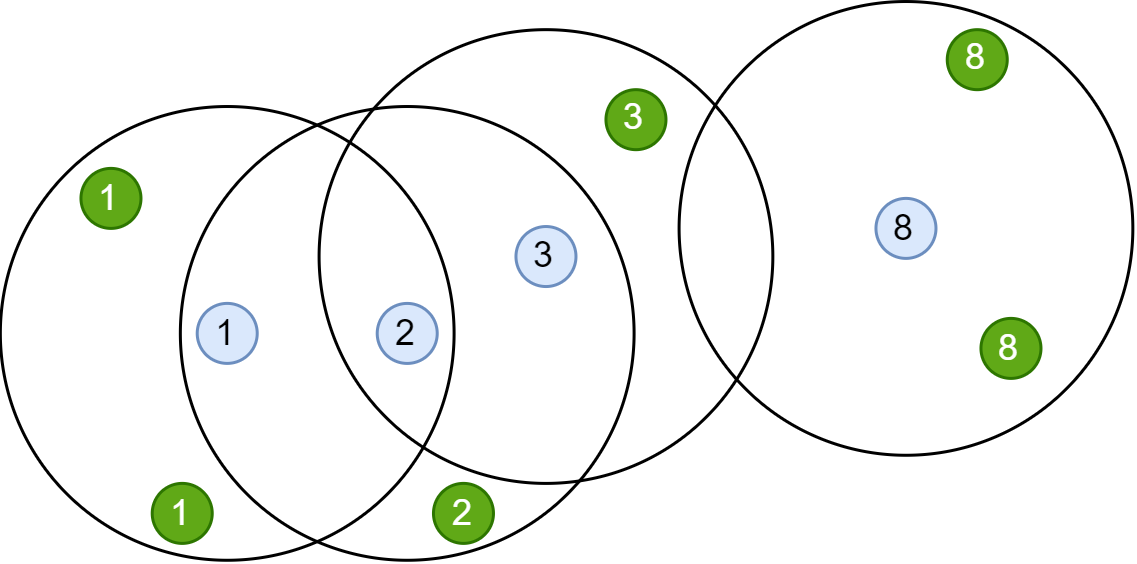
\includegraphics[width=\linewidth]{img/redbscan.png}
		\caption{处理边界对象}
		\label{redata2}
	\end{minipage}
\end{figure}

经过上述处理,使得边界对象的划分结果稳定,与最近的核心对象所属簇保持一致。同时减少了聚类算法的计算复杂度,无需再对边界对象的簇标识进行处理,只要记录相邻关系,最后还原即可。

本方案包含三个步骤,初始化、聚类以及还原结果。还原结果的过程与章节\ref{task1-huanyuan}所述方式完全一致,这里不多做说明。主要区别在于初始化和聚类过程,下面将着重介绍这两个部分。

\subsection{初始化}
不同于方案一的初始化过程,这里需要对每个非核心对象求最近的核心对象,并修改cluId,与最近的核心对象保持一致。上述操作需要运行安全极值协议,计算和通信开销相较于方案一的预处理过程略微增加。

具体流程如算法\ref{alg_t2_s1}所示。首先,计算每个元素到其他元素的距离,同时获取邻域关系存储在$ u $中,并且记录每个元素邻域范围内包含点的个数$ s[j],j\in[n] $。然后,并行比较$ s $与minPts的大小关系,并更新每个元素的isCore属性。

计算完isCore信息后,开始本节算法的核心部分,即更新非核心对象的cluId。
预设标识$ m $来判断是否对元素$ x[i] $更新cluId,判断依据是若$ x[i] $为非核心对象并且邻域范围内存在核心对象,则可以修改。若$ x[j] $为核心对象且与$ x[i] $相邻,则$ t1[j] $为1,否则$ t2[j] $为1。
对所有元素进行遍历之后,若$ m=1 $则代表$ \epsilon $邻域内存在核心对象,否则不存在。此时通过乘法排除$ x[i] $为核心对象的情况,若为核心对象则无论邻域内是否有其他核心对象均不修改cluId。
根据$ t1 $、$ t2 $以及距离值,计算出$ r1 $,过滤出所有相邻核心对象的距离,无关对象的距离设为最大值$ max $,避免影响求解距离最近的核心对象。
最后,通过逐个相乘后累加来求解最近相邻核心对象的cluId,并根据前述$ m $值来控制是否更新cluId。

\begin{algorithm}[htbp]
	\renewcommand{\algorithmicrequire}{\textbf{输入:}}
	\renewcommand{\algorithmicensure}{\textbf{输出:}}
	\caption{初始化}
	\label{alg_t2_s1}
	\begin{algorithmic}[1]
		\REQUIRE 数组sharedList简写为x
		\ENSURE 距离关系$ u $
		\FOR {$ i=1 $ to $ n $}
		\FOR {$ j=1 $ to $ n $}
		\STATE $ d[j] \leftarrow \text{DIST}(x[i].data, x[j].data) $
		\ENDFOR
		\STATE $ u[i] \leftarrow \text{SC}(d,[\epsilon]_n) $
		\STATE $ s[i] \leftarrow \text{sum}(u[i][j])\ \text{for}\ j\in[n]$
		\ENDFOR
		\STATE $ r \leftarrow \text{SC}([minPts]_n,s) $
		\STATE x[i].isCore $\leftarrow r[i]\ \text{for}\ i\in[n] $
		\FOR {$ i=1 $ to $ n $}
		\STATE $ m \leftarrow 0 $
		\FOR{$ j=1 $ to $ n $}
		\STATE $ t1[j] \leftarrow \text{MUL}(x[j].isCore, u[i][j]) $
		\STATE $ t2[j] \leftarrow 1-t1[j] $
		\STATE $ m = t1[j] + m - \text{MUL}(m, t1[j]) $
		\ENDFOR
		\STATE $ m \leftarrow \text{MUL}(m, 1-x[i].isCore) $
		\STATE $ r1 \leftarrow \text{MUL}(d, t1) + \text{MUL}([max]_n, t2) $
		\STATE $ r2 \leftarrow \text{SMin}(r1) $
		\STATE $ nId \leftarrow \text{sum}(\text{MUL}(r2[j], x[j].cluId))\ \text{for}\ j \in [n] $
		\STATE $ x[i].cluId \leftarrow \text{MUL}(nId, m) + \text{MUL}(1-m, x[i].cluId)$
		\ENDFOR
	\end{algorithmic}
\end{algorithm}

值得一提的是,对于核心对象,$ m = 0 $无需修改cluId。对于边界对象,依据算法将修改cluId与最近相邻核心对象保持一致。对于噪声$ m=0 $,因此cluId不会发生改变。

\subsection{核心对象聚类}
在初始化的过程中,所有边界元素均已被划分到最近相邻核心对象所属簇中,因此相较于方案一中的聚类过程(见算法\ref{alg_t1_s2}),本方案的聚类过程更加简单便捷。
在算法\ref{alg_t2_s2}中只要记录相连的临时簇信息即可,当且仅当x[i]与x[j]均为核心对象并且距离小于$ \epsilon $,则认为二者相连。
%算法的复杂度为$ O(n^2) $,仅涉及简单的乘法操作,聚类效率较高。
\begin{algorithm}[htbp]
	\renewcommand{\algorithmicrequire}{\textbf{输入:}}
	\renewcommand{\algorithmicensure}{\textbf{输出:}}
	\caption{聚类}
	\label{alg_t2_s2}
	\begin{algorithmic}[1]
		\REQUIRE 数组sharedList简写为x,相邻关系$ u[i][j],i,j\in[n] $
		\ENSURE 相连关系$ plist $
		\FOR {$ i=1 $ to $ n $}
		\FOR {$ j=1 $ to $ n $}
		\STATE $ r \leftarrow \text{MUL}(x[i].isCore, x[j].isCore, u[i][j]) $
		\STATE 新增元素info(x[i].cluId, x[j].cluId, r)到plist中
		\ENDFOR
		\ENDFOR
	\end{algorithmic}
\end{algorithm}

\section{基于DBSCAN的隐私保护层次聚类}
\label{s4-t3}
方案一(\ref{s4-t1}节)和方案二(\ref{s4-t2}节)均是在用户给出$\epsilon$和minPts值的基础上,实现隐私保护DBSCAN。但是现实情况中,多个独立用户协同聚类时,不知道彼此拥有的具体数据信息,难以根据数据分布特点给出适合的参数,从而导致聚类效果较差。

为了解决上述问题,尽可能减少用户对聚类的影响,本节根据论文\cite{latifi2021dbhc}中的思想设计了一种基于DBSCAN的隐私保护层次聚类方案。前述方案的$\epsilon$均为固定值,没有考虑到数据集中的数据密度可能不同这一情况,导致在个别数 据集上划分效果不佳的问题。本方案考虑数据集密度不同的特点,设置不同的$\epsilon$值进行聚类以提升聚类效果。

整个方案主要可以分为三个阶段:
\begin{compactitem}
	\item \textbf{获取$\epsilon$值}:云服务器协同通过计算数据之间的距离,绘制$ k $线图并固定间隙取值来计算系列$\epsilon$值。
	\item \textbf{计算初始簇}:云服务器根据上述获取的$\epsilon$值,升序取$ \epsilon $并据此反复执行DBSCAN过程,已被划分的点不再参与后续过程,直到遍历完所有$\epsilon $的值。
	\item \textbf{合并初始簇}:在初始簇的基础上,用户不断将相距最近的初始簇进行合并,直到簇个数满足要求$ k $个,即得到最终簇划分结果。
\end{compactitem}

\subsection{获取$\epsilon$值}
%todo 修改下排版
本小节将详细阐述如何通过$ k $线图来获取所有聚类所需的$\epsilon$值,$ k $线图的绘制方式为,首先计算每个点到其最近的第$ k $个点的距离,然后按照升序方式排列,最后根据这些排序值绘图。在算法\ref{alg_t3_s1}中,将详细说明计算流程。

由于真实数据集的复杂性,目前没有办法准确找到每个数据集具体包含多少种不同的密度,DBHC方案\cite{latifi2021dbhc}经过分析,选择在$ k $线图中固定间隔来选取$\epsilon$的值,数据集的大小为$ n $,则间隔为$ \sqrt{n} $。因此DBSCAN的执行次数也为$ \sqrt{n} $次。

\begin{algorithm}[htbp]
	\renewcommand{\algorithmicrequire}{\textbf{输入:}}
	\renewcommand{\algorithmicensure}{\textbf{输出:}}
	\caption{获取$\epsilon$值}
	\label{alg_t3_s1}
	\begin{algorithmic}[1]
		\REQUIRE 秘密共享的元素数组$ \{x[1],...,x[n]\} $
		\ENSURE 秘密共享的$\epsilon$值$ elist $
		\FOR {$ i=1 $ to $ n $}
		\FOR {$ j=i+1 $ to $ n $}
		\STATE $ d[i][j] \leftarrow \text{DIST}(x[i].data, x[j].data) $
		\STATE $ d[j][i] \leftarrow d[i][j] $
		\ENDFOR
		\ENDFOR
		\FOR{$ i=1 $ to $ n $}
		\STATE $ r \leftarrow \text{SMin}(d[i]) $ % 求解最近距离
		\STATE $ t[j] \leftarrow 1-r[j] $ for $ j\in[n] $
		\STATE $ d[i] \leftarrow \text{MUL}(d[i], t) + \text{MUL}([max]_n, r) $
		\STATE $ r \leftarrow \text{SMin}(d[i]) $
		\STATE $ d2[i] \leftarrow \text{sum}(\text{MUL}(d[i], r)) $ % 获取第二近的距离
		\ENDFOR
		\STATE $ sdist \leftarrow \text{SSORT}(d2) $
		\STATE $ j \leftarrow \text{sqrt}(n) $
		\FOR {$ i=j $ to $ n $}
		\STATE 添加 $ sdist[i] $ 到elist中
		\STATE $ i \leftarrow i + j $
		\ENDFOR
	\end{algorithmic}
\end{algorithm}

首先,计算元素与元素之间的距离,由于距离是相对的$ d[i][j]=d[j][i] $,因此缩减了一半的计算量。然后,取$ k=2 $,计算每个点第二近的距离来绘制$ k $线图。$ d $为二维矩阵,$ d[i] $存储元素$ i $所有距离值,首先求距离最小值,然后通过乘法和加法使得$ d[i] $中的最小值化为最大值,在此之后,再求解一次最小值,即可获得第$ k $小的值。
通过乘法使得数组中只保留第2小的值,其他值均为0,然后通过计算数组累加值来获取最终结果存储到数组$ d2 $中。其中,借助安全排序算法来对$ d2 $数组进行升序排列,结果存放到$ sdist $中。

值得一提的是,这里的固定间隙值$ \sqrt{n} $在明文上进行计算,因为数据集的大小$ n $对于云平台是已知的。最后,从$ sdist $中按照固定间隙$ \sqrt{n} $取$\epsilon$的值存储到$ elist $中并返回结果。当k线图中的k取其他值时,只需要增加求解最小值的次数,遵循算法中的处理步骤即可获得相应结果,这里不再赘述。


\subsection{计算初始簇}
本节将详细介绍,如何在获取了所有$\epsilon$值后对不同密度的数据进行聚类。算法的基本逻辑是,对每个$\epsilon$值(按升序)执行一次DBSCAN算法,总共$|E|$次。$\epsilon$值较小时,无法覆盖所有数据,因此剩余部分数据没有被划分,为了使剩余数据被划分的同时,已经划分的数据不受影响,将这些数据移出数据集。经过上述过程会产生较多簇,在下一节,将进行合并操作以获取预期的聚类划分结果。在算法\ref{alg_t3_s2}中,将详细说明密文方案中计算初始簇的方式。

\begin{algorithm}[htbp]
	\renewcommand{\algorithmicrequire}{\textbf{输入:}}
	\renewcommand{\algorithmicensure}{\textbf{输出:}}
	\caption{计算初始簇}
	\label{alg_t3_s2} % task3 step2
	\begin{algorithmic}[1]
		\REQUIRE 秘密共享的元素数组$ \{x[1],...,x[n]\} $,秘密共享的$\epsilon$值$ elist $
		\ENSURE 初始簇列表cluList
		\FOR{each $\epsilon$ in $elist$}
		% 初始信息更新
		\FOR {$i=1$ to $n$}
		\STATE $x[i].isCore \leftarrow 0$ %清空之前的corepoint计算结果
		\FOR {$j=1$ to $ n$}
		\STATE $t \leftarrow ( 1- x[j].isMark) * (1-x[i].isMark)$
		\STATE $d^{\prime}[j] \leftarrow \text{MUL}(t,d[i][j])+\text{MUL}(1-t,max)$
		\ENDFOR
		\STATE $u[i] \leftarrow \text{SC}(d^{\prime},[\epsilon]_n)$
		\STATE $nei[i] \leftarrow \text{sum}(u[i])$
		\ENDFOR
		\STATE $r \leftarrow \text{SC}([minPts]_n, nei)$
		\STATE $x[i].isCore \leftarrow r[i]$ for $i\in[n]$
		\STATE 执行算法\ref{alg_t3_s2-2}进行聚类
		\ENDFOR
	\end{algorithmic}
\end{algorithm}

根据算法\ref{alg_t2_s2}排序所得$\epsilon$值为升序排列,因此这里不再进行排序操作,直接遍历elist,针对每个$\epsilon$值进行聚类即可。
首先,进行数据处理工作,在每次聚类前将数据的isCore信息清空置0。然后计算$x[i]$与$x[j]$之间的距离,$d[i][j]$在获取$\epsilon$值时已经算出,无需重复计算。只有当$x[i]$与$x[j]$均没有被划分($x[i].isMark=0,x[j].isMark=0$)时,距离为$d[i][j]$,否则为数值范围内最大值$max$。
然后,比较距离和$\epsilon$大小关系,并记录到$u$中,同时累加邻域范围内的点记录到$nei$中。
最后,比较邻域范围内点个数与minPts的大小关系,并据此更新$x[i]$的isCore属性。
最后根据上述信息,执行DBSCAN聚类。

在算法\ref{alg_t3_s2-2}中将详细解释执行聚类的过程。
首先判断是否更新x[j].cluId,计算标识m1。更新依据为,当且仅当x[i]为未标记核心对象(x[i].isCore=1,x[i].isMark=0)并且x[j]为未标记非核心对象(x[j].isCore=0,x[j].isMark=0)且二者相邻(u[i][j]=1)时,有m1=1,修改x[j]的cluId与x[i]保持一致。
然后记录相邻关系,当且仅当x[i]与x[j]均为未标记核心点且二者相邻时,有m2=1,将信息记录到plist中。
最后更新x[j]的isMark标识,这里实现的是逻辑或关系,若x[j]已经被标记(x[j].isMark=1)或者在本次迭代中被标记(m1=1),则x[j].isMark=1。注意这里只有非核心对象会更新。
在遍历完所有点后,再对核心对象更新一次isMark标识,上述迭代过程中,只有未被标记的非核心对象会更新isMark标识,这里引入新一轮操作,对所有核心对象更新标识。以防止在下一次聚类过程中,出现已经聚类过的核心对象。

\begin{algorithm}[htbp]
	\renewcommand{\algorithmicrequire}{\textbf{输入:}}
	\renewcommand{\algorithmicensure}{\textbf{输出:}}
	\caption{聚类}
	\label{alg_t3_s2-2} % task3 step2
	\begin{algorithmic}[1]
		\REQUIRE 秘密共享的元素数组$ \{x[1],...,x[n]\} $
		\ENSURE 更新信息后的元素数组
		\FOR{$i=1$ to $n$}
		\FOR{$j=1$ to $n$}
		\STATE $ m1 \leftarrow \text{MUL}(x[i].isCore,1-x[i].isMark, 1- x[j].isCore, 1-x[j].isMark, u[i][j]) $
		\STATE $x[j].cluId \leftarrow \text{MUL}(m1, x[i].cluid) + \text{MUL}(1-m1, x[j].cluId)$
		\STATE $ m2 \leftarrow \text{MUL}(x[i].isCore, 1-x[i],isMark, x[j].isCore, 1-x[j].isMark, u[i][j]) $
		\STATE 记录新的元素(x[i].cluId, x[j].isCore, m2)到plist中
		\STATE $ x[j].isMark \leftarrow x[j].isMark + m1 - \text{MUL}(x[j].isMark, m1) $
		%		\STATE $ t1 \leftarrow  \text{MUL}(x[i].isCore,1-x[i].isMark)$
		%		\STATE $ t2 \leftarrow \text{MUL}(u[i][j],1-x[j].isMark) $
		%		\STATE $ t3 \leftarrow \text{MUL}(t2, 1-x[j].isCore)$
		%		\STATE $ t \leftarrow \text{MUL}(t1, t3) $
		%		\STATE $x[j].cluId \leftarrow \text{MUL}(t, x[i].cluid) + \text{MUL}(1-t, x[j].cluId)$
		%		\STATE $m[j] \leftarrow m[j] + t - \text{MUL}(m[j], t)$
		%		% record pair info
		%		\STATE $r \leftarrow \text{MUL}(t, x[j].isCore)$
		%		\STATE 记录新的元素(x[i].cluId, x[j].isCore, r)到plist中
		\ENDFOR
		\ENDFOR
		\FOR{$i=1$ to $n$}
		\STATE  x[i].isMark $ \leftarrow $ x[i].isCore+x[i].isMark - \text{MUL}(x[i].isCore,x[i].isMark)
		\ENDFOR
		
	\end{algorithmic}
\end{algorithm}

%首先更新数据的cluId,只有在$x[i]$为未被标记的核心点,$x[j]$未被标记,且二者相邻$u[i][j]=1$的情况下,才将$x[j]$的cluId修改为与$x[i]$一致。
%$ m[j] $记录是否更新$x[j]$的isMark信息,若$x[j]$的cluId被修改过,则认为该数据已被被划分。
%然后,记录核心点相连信息,在上述判断是否修改cluId逻辑的基础上,加入$x[j]$为核心点的限制即可,随后构造新元素并将结果计入plist中。
%最后,更新所有元素的isMark属性,若元素在之前聚类过程中已被聚类(isMark=1)或者在本次聚类中被划分(m[i]=1),则isMark属性标记为1。
%isMark的作用是让本轮以及之前被划分好的数据不再参与后续聚类。
\begin{algorithm}[htbp]
	\renewcommand{\algorithmicrequire}{\textbf{输入:}}
	\renewcommand{\algorithmicensure}{\textbf{输出:}}
	\caption{合并初始簇}
	\label{alg_t3_s3}
	\begin{algorithmic}[1]
		\REQUIRE 秘密共享的聚类结果$plist$,期望簇个数$k$
		\ENSURE $k$个簇信息
		\STATE 根据\ref{alg_t1_s3}还原聚类结果得到获取resCId的plist
		\STATE 根据plist获取初始簇集合$ C $,每个簇包含的数据个数num和中心cen
		\STATE 开始合并初始簇
		\WHILE{$ |C| > k$}
		\STATE 计算簇与簇之间的距离$d$
		\STATE 求解距离最近的两个簇$c_a$和$c_b$进行合并
		\STATE 更新簇参数num和cen
		\ENDWHILE
	\end{algorithmic}
\end{algorithm}
\subsection{合并初始簇}
本节的主要工作由用户独立完成,在算法\ref{alg_t3_s3}中给出详细描述。
首先根据算法\ref{alg_t1_s3}将临时簇进行合并还原成初始簇,并更新plist每个数据的resCId,即初始簇标识,然后对plist进行处理获取每个初始簇包含点的个数以及簇中心。反复求解集合$ C $中最近的两个簇$ c_a $和$ c_b $然后将数据进行合并,更新参数直到簇的个数为$ k $个。每一次合并初始簇,$ |C| $的值都会减少一个。合并簇的过程不仅需要更新数据个数num和簇中心cen,也要更新对应数据的resCId。
%\section{安全性分析}
%\label{s4-lilun}
\section{实验评估}
\label{s4-shiyan}
在本节中,我们基于C++编程语言和SCI函数库\cite{rathee2020cryptflow2}实现了三个方案,将分别给出隐私保护DBSCAN(方案一)、改进的隐私保护DBSCAN(方案二)以及基于DBSCAN的隐私保护层次聚类(方案三)的实验分析结果。本文将会在多个数据集上进行实验,从聚类的质量和运行效率两方面进行对比,此外实验结果会与其他隐私保护DBSCAN相关研究\cite{bozdemir2021privacy}以及隐私保护K-means相关研究\cite{mohassel2019practical}进行对比来说明本文方案的实用性和高效性。

%\subsection{理论分析}
%本小节,对上述三个方案给出对应的复杂度分析,方案主要有安全计算子协议组成,例如安全比较(SC)、安全排序(SSORT)以及安全乘法(MUL)等。其中安全排序和安全极值协议由安全比较和安全乘法组成。因此将方案进行拆分,可以分为安全比较协议和安全乘法协议两部分。
%
%安全比较协议基于百万富翁协议\cite{rathee2020cryptflow2},计算与通信均比较复杂。安全乘法协议根据Beaver乘法三元组\cite{beaver1992efficient}实现,其中预计算的内容均由用户或者第三方机构离线产生,不产生聚类开销,与安全比较协议相比,运算开销较小。因此在下面的分析过程中,以安全比较协议的执行次数来衡量方案的复杂度,省略乘法次数的分析。
%
%具体的比较如下图\ref{s4-table-lilunfenxi}所示:
%
%\begin{table}[htbp]
%	\centering
%	\renewcommand{\arraystretch}{1.3}
%	\caption{方案复杂度理论分析}
%	\scalebox{1.0}{
%		\begin{tabular}{c|c|c|c}% 通过添加 | 来表示是否需要绘制竖线c|
%			\hline  % 在表格最上方绘制横线
%			方案     & 方案一  & 方案二   & 方案三             \\
%			\hline % 在表格最下方绘制横线
%			比较次数 & $ n+1 $ & $ 2n+1 $ & $3n+\sqrt{n}(n+1)$ \\%$n^2\log n$
%			\hline
%		\end{tabular}
%	}
%	\label{s4-table-lilunfenxi}
%\end{table}
%
%安全比较协议一次可以比较多对数据,在安全极值协议中,给出了两种实现方式,分别是小数据量上的最值协议和大数据量上的树状比较,前者通过增加比较数据对减少比较次数,$ n $个数据构造$ n^2 $个比较对,进行一轮比较,后者通过树状比较结构减少比较对数,进行$ \log n $轮比较。
%在本节的分析中,选择基于小数据量上的比较,因此运行一次安全极值协议进行一次安全比较。
%
%从表格中可以看到,方案二相比方案一复杂度没有量级上的差异,因此在后面的实验中也可以看到开销的差异并不是非常显著。但是方案三的复杂度则提升了一个量级,因此开销大大增加。
%具体的耗时对比,会在下面的实验中给出。
\subsection{实验设置}
\textbf{服务器配置:}在一台主机上模拟两个云平台进行交互,机器的配置为Inter Core i7-7700HQ 2.80 GHz CPU和16 GB RAM。

\textbf{场景:}隐私保护DBSCAN方案既可以应用于外包计算也可以应用于两方安全计算的场景。此外,聚类的数据可以采取任意划分形式,例如水平划分、垂直划分或者是混合划分。在以下实验中,基于外包计算的场景,用户将数据秘密共享后分别发送给两个不共谋的云服务器。值得一提的是,外包计算场景下,参与聚类的用户数量不受限制,实验中假设单个用户上传所有数据。方案可以直接应用到用户更多的场景中,只要数据、参数和簇个数和实验保持一致即可。

\textbf{数据集:}为了更好地评估聚类方案,本文在多个不同的数据集上进行了实验。其中Lsun与S1数据集是为了和论文\cite{bozdemir2021privacy}对比方案的效率和实用性。

\begin{compactitem}
	\item \textbf{Lsun:}图\ref{fig:a}中的Lsun数据集\cite{ultsch2005clustering}在论文\cite{wu2020secure,bozdemir2021privacy}分别用于评估隐私保护K-means和隐私保护DBSCAN方案的性能。它的正确划分结果中包含3个簇,分别拥有不同的方差和簇距离。三个簇分别包含200、100和100个元素,彼此没有重叠的部分。
	\item
	\textbf{S1:}图\ref{fig:c}中的S1数据集\cite{franti2018k}是一个人工合成的二维数据集,包含5000个样本,可以划分为15个不同的球形高斯簇,分别包含300到350个元素。其中簇之间有9\%的重叠部分。该数据集在论文\cite{bozdemir2021privacy,mohassel2019practical,su2007privacy}中被用于分析聚类效果。
	\item
	\textbf{Aggregation:}图\ref{fig:e}中的Aggregation数据集\cite{gionis2007clustering}为人工合成的二维数据集,包含788个数据,7个分类。在后续实验中,将通过该数据集分析K-means和DBSCAN聚类结果的差异,数据之间有极少重叠部分。
	\item
	\textbf{合成数据集:}图\ref{fig:dd}为实验构造包含不同密度数据的二维数据集,用来衡量三个方案在多密度数据集上的聚类效果。为了方便观察和对比分析,数据集包含数据量较少,分布较简单,不同簇之间的密度差异较大。其中分别包含3个簇,C1密度最大,C3密度最小而C2的密度在二者之间。实验中,$ \epsilon $设置不同值,观察最终划分结果。
\end{compactitem}

\begin{figure}[htbp]
	\centering
	\subfloat[\label{fig:a}]{
		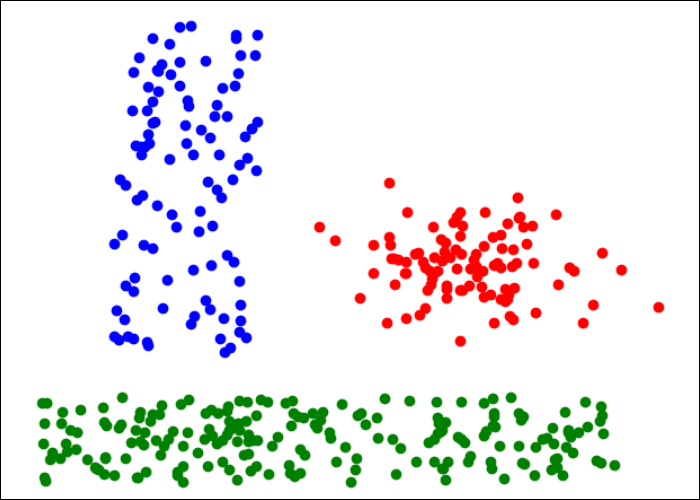
\includegraphics[width=.45\textwidth]{img/lsun_gt.png}}
	\subfloat[\label{fig:c}]{
		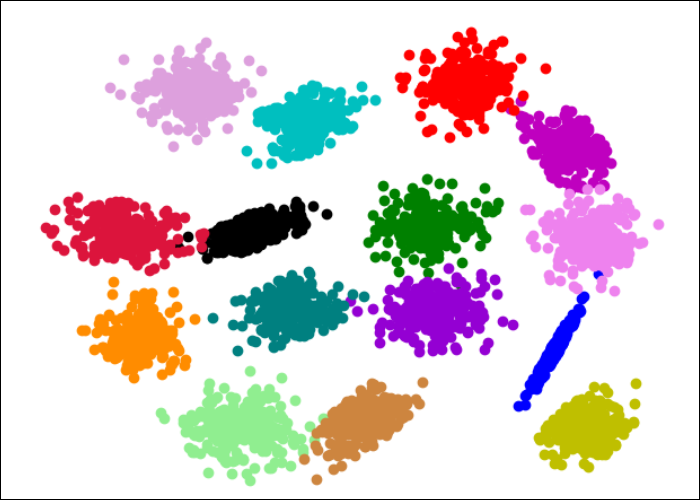
\includegraphics[width=.45\textwidth]{img/s1_gt.png}}
	\\
	\subfloat[\label{fig:e}]{
		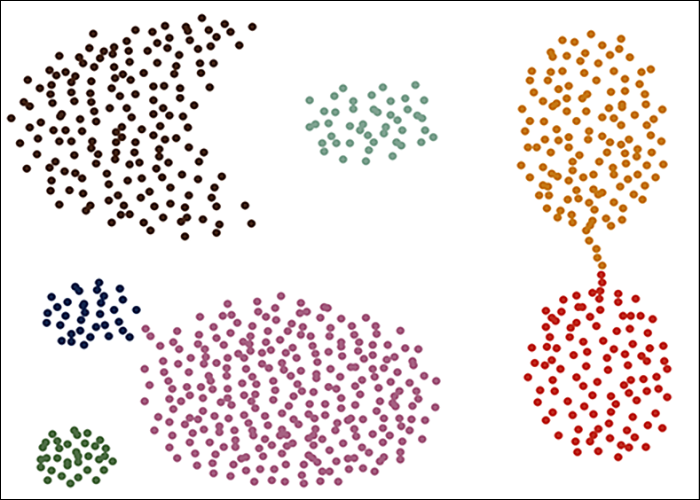
\includegraphics[width=.45\textwidth]{img/aggre_gt.png}}
	\subfloat[\label{fig:dd}]{
		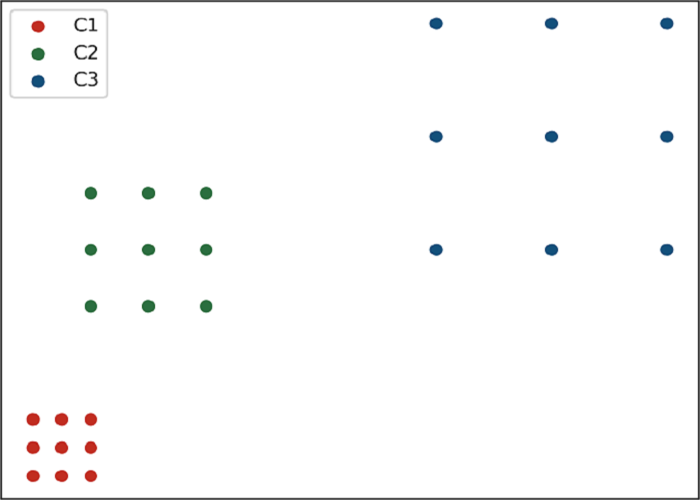
\includegraphics[width=.45\textwidth]{img/expnew.png}}
	\caption{Lsun、S1、Aggregation以及合成数据集正确划分结果}
\end{figure}

\textbf{编码:}Lsun数据集由有理数组成。参考前述工作\cite{jaschke2019unsupervised},将数据放大$ 10^6 $全部转化为整数后执行协议。相应的,Aggregation数据集放大$ 10^2 $倍,S1数据集由整数构成不进行放缩,合成数据集的数据均为整数。

\begin{table}[htbp]
	\centering
	\renewcommand{\arraystretch}{1.3}
	\caption{数据集参数设置详细信息}
	\scalebox{1.0}{
		\begin{tabular}{c|c|c|c|c|c}% 通过添加 | 来表示是否需要绘制竖线c|
			\hline  % 在表格最上方绘制横线
			数据集      & 维度 & 簇个数 & 数据量 & $\epsilon$          & minPts \\
			\hline % 在表格最下方绘制横线
			Lsun        & 2    & 3      & 400    & $ 2\times 10^{11} $ & 4      \\%$n^2\log n$
			\hline
			S1          & 2    & 15     & 5000   & $ 2.25\times 10^9 $ & 50     \\
			\hline
			Aggregation & 2    & 7      & 788    & $ 3.5\times 10^4 $  & 3      \\
			\hline
			人造数据集 & 2 & 3 & 27 & - & 3 \\
			\hline
		\end{tabular}
	}
	\label{s4-table-dataset}
\end{table}

\textbf{参数:}方案一与方案二均需要人工设定$\epsilon$和minPts的值,参考论文\cite{bozdemir2021privacy}中的设置,并根据编码过程中的放缩值对参数进行修改,同时,由于算法中计算欧式距离去掉了根号,因此也对$\epsilon$值做出了相应的处理。
具体信息在表格\ref{s4-table-dataset}中给出。
方案三不需要提前根据数据特点分析给出$\epsilon$和minPts的值,在本节的实验中,目标簇个数$ k $根据数据集的正确簇划分结果给出。

\subsection{性能分析与测试}
\subsubsection{聚类质量分析}
% 主要是衡量下ari指标以及聚类结果展示对比
本小节,将根据调整兰德系数(ARI)在Lsun、S1和Aggregation数据集上进行实验来比较上述几个方案与论文\cite{bozdemir2021privacy}中提出的ppDBSCAN方案以及明文标准K-means算法的聚类质量。

由于聚类是一种无监督机器学习算法,没有办法计算准确率,但是Lsun、S1与Aggregatin为人工合成数据集,主要用于对机器学习算法进行基准测试,所以正确的分类结果是已知的。因此,能够基于这些数据集对聚类算法用ARI指标来衡量聚类质量,这是一个广泛应用的外部聚类质量指标\cite{vinh2009information,arbelaitz2013extensive},详细的计算方法在小节\ref{s4-ari-intro}给出。
\begin{table}[htbp]
	\centering
	\renewcommand{\arraystretch}{1.3}
	\caption{聚类质量评估}
	\scalebox{1.0}{
		\begin{tabular}{c|c|c|c|c|c}% 通过添加 | 来表示是否需要绘制竖线c|
			\hline  % 在表格最上方绘制横线
			数据集      & K-means & ppDBSCAN\cite{bozdemir2021privacy} & 方案一 & 方案二 & 方案三 \\
			\hline % 在表格最下方绘制横线
			Lsun        & 0.4386  & 1.0                                & 1.0    & 1.0    & 0.3779 \\%$n^2\log n$
			\hline
			S1          & 0.9254  & 0.9757                             & 0.9766 & 0.9778 & 0.9510 \\
			\hline
			Aggregation & 0.7621  & -                                  & 0.8089 & 0.8089 & 0.8049 \\
			\hline
		\end{tabular}
	}
	\label{s4-table-arires}
\end{table}

为了进行公平合理的比较,对每个方案都选择了最佳的参数设置。对于K-means,选择sklearn库中的标准K-means聚类方法来获取结果\cite{buitinck2013api},提供准确的簇个数,同时为了使算法更快收敛和获取高质量的K-means聚类结果,选择K-means++参数来优化初始簇中心的选择(另一种选择为设置random参数,随机选择初始簇中心)。对于DBSCAN,按照表格\ref{s4-table-dataset}来设置参数运行所有方案。论文\cite{bozdemir2021privacy}没有给出基于Aggregation的实验结果,因此这里不进行对比分析。在表格\ref{s4-table-arires}中,可以看到基于ARI的聚类质量评估结果。

\begin{compactitem}
	\item \textbf{与K-means比较:}在所有数据集上,本文所述方案一和方案二的划分结果均优于K-means聚类的划分结果,方案三在Lsun数据集上的聚类效果较差。在Lsun这种非球形数据集上,K-means的聚类质量较差。S1主要包含球形数据集,因此K-means方案的划分结果的ARI值与方案一二三相近。Aggregation数据集同时包含球形和非球形的数据集,因此方案一二三比K-means表现更好。值得一提的是,K-means算法的聚类效果受到初始簇中心的影响较大,若随机生成初始簇中心,ARI指标的计算值会更小。
	\item
	\textbf{与ppDBSCAN比较:}这里将方案一的聚类质量与ppDBSCAN进行对比分析,因为方案一和ppDBSCAN都是基于传统DBSCAN算法,聚类效果应当与明文DBSCAN一致。但是方案一在S1数据集上表现更好,具体来说可能有几方面的原因。首先是S1数据集有部分重叠,论文\cite{bozdemir2021privacy}为了简化密文方案复杂度,没有完全遵循明文DBSCAN的思路,设置了最大迭代深度来限制次数,该参数主要受到数据分布影响,可能会影响聚类结果。其次,数据集的顺序对DBSCAN的划分效果会产生影响,因此即便是ppDBSCAN的迭代深度设置正确,二者最终划分结果也可能会出现一些差异。
	\item
	\textbf{方案一二三比较:}在Lsun数据集上,方案一二结果一致,均能够正确划分簇,但是方案三聚类效果较差,原因可能是根据系列eps值聚类,会导致产生很多初始簇,按照最近簇合并的方式,可能会导致某些数据集上划分效果较差。在S1这种包含重叠部分的数据集上,方案二的表现最好,原因在于该方案能够获取稳定的数据划分结果,使得在数据集包含较多重叠部分时,让边界对象划分到最近的核心对象所属簇中,提升聚类质量。方案三在包含不同密度数据的数据集上表现会更好,虽然能够自适应选择关键参数,但是适用场景有限,开销较大。
\end{compactitem}

\textbf{可视化比较:}图\ref{s4-img-clures}中,给出了聚类的可视化结果,行依次对应Lsun、S1和Aggregation数据集,列依次为方案一、二、三和明文K-means的聚类结果。其中黑色为DBSCAN结果中的噪声点。可以看到方案一二均划分的较好,但是方案三在簇内部产生较多噪声点,划分结果产生一些误差。K-means在非球形数据集上容易将单一簇划分为两个,效果较差(\ref{s4-img-clures}.d/\ref{s4-img-clures}.l)。对比图\ref{s4-img-clures}.e和\ref{s4-img-clures}.f可以看到在不同簇之间的重叠部分划分结果不一样,方案二打乱数据后,重复运行结果保持一致,方案一则会产生变化。

\begin{figure}[htb]
	\centering
	\subfloat[]{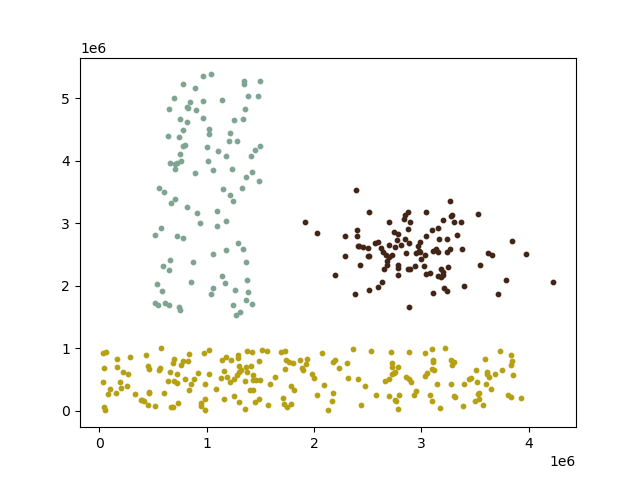
\includegraphics[width=.25\textwidth]{img/t1-lsun.png}}
	\subfloat[]{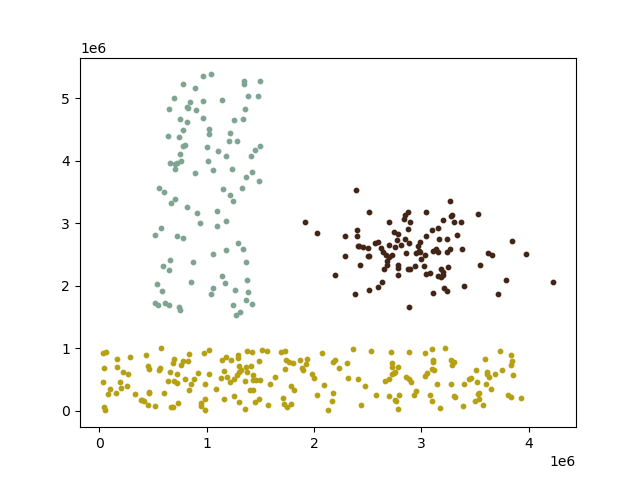
\includegraphics[width=.25\textwidth]{img/t2-lsun.png}}
	\subfloat[]{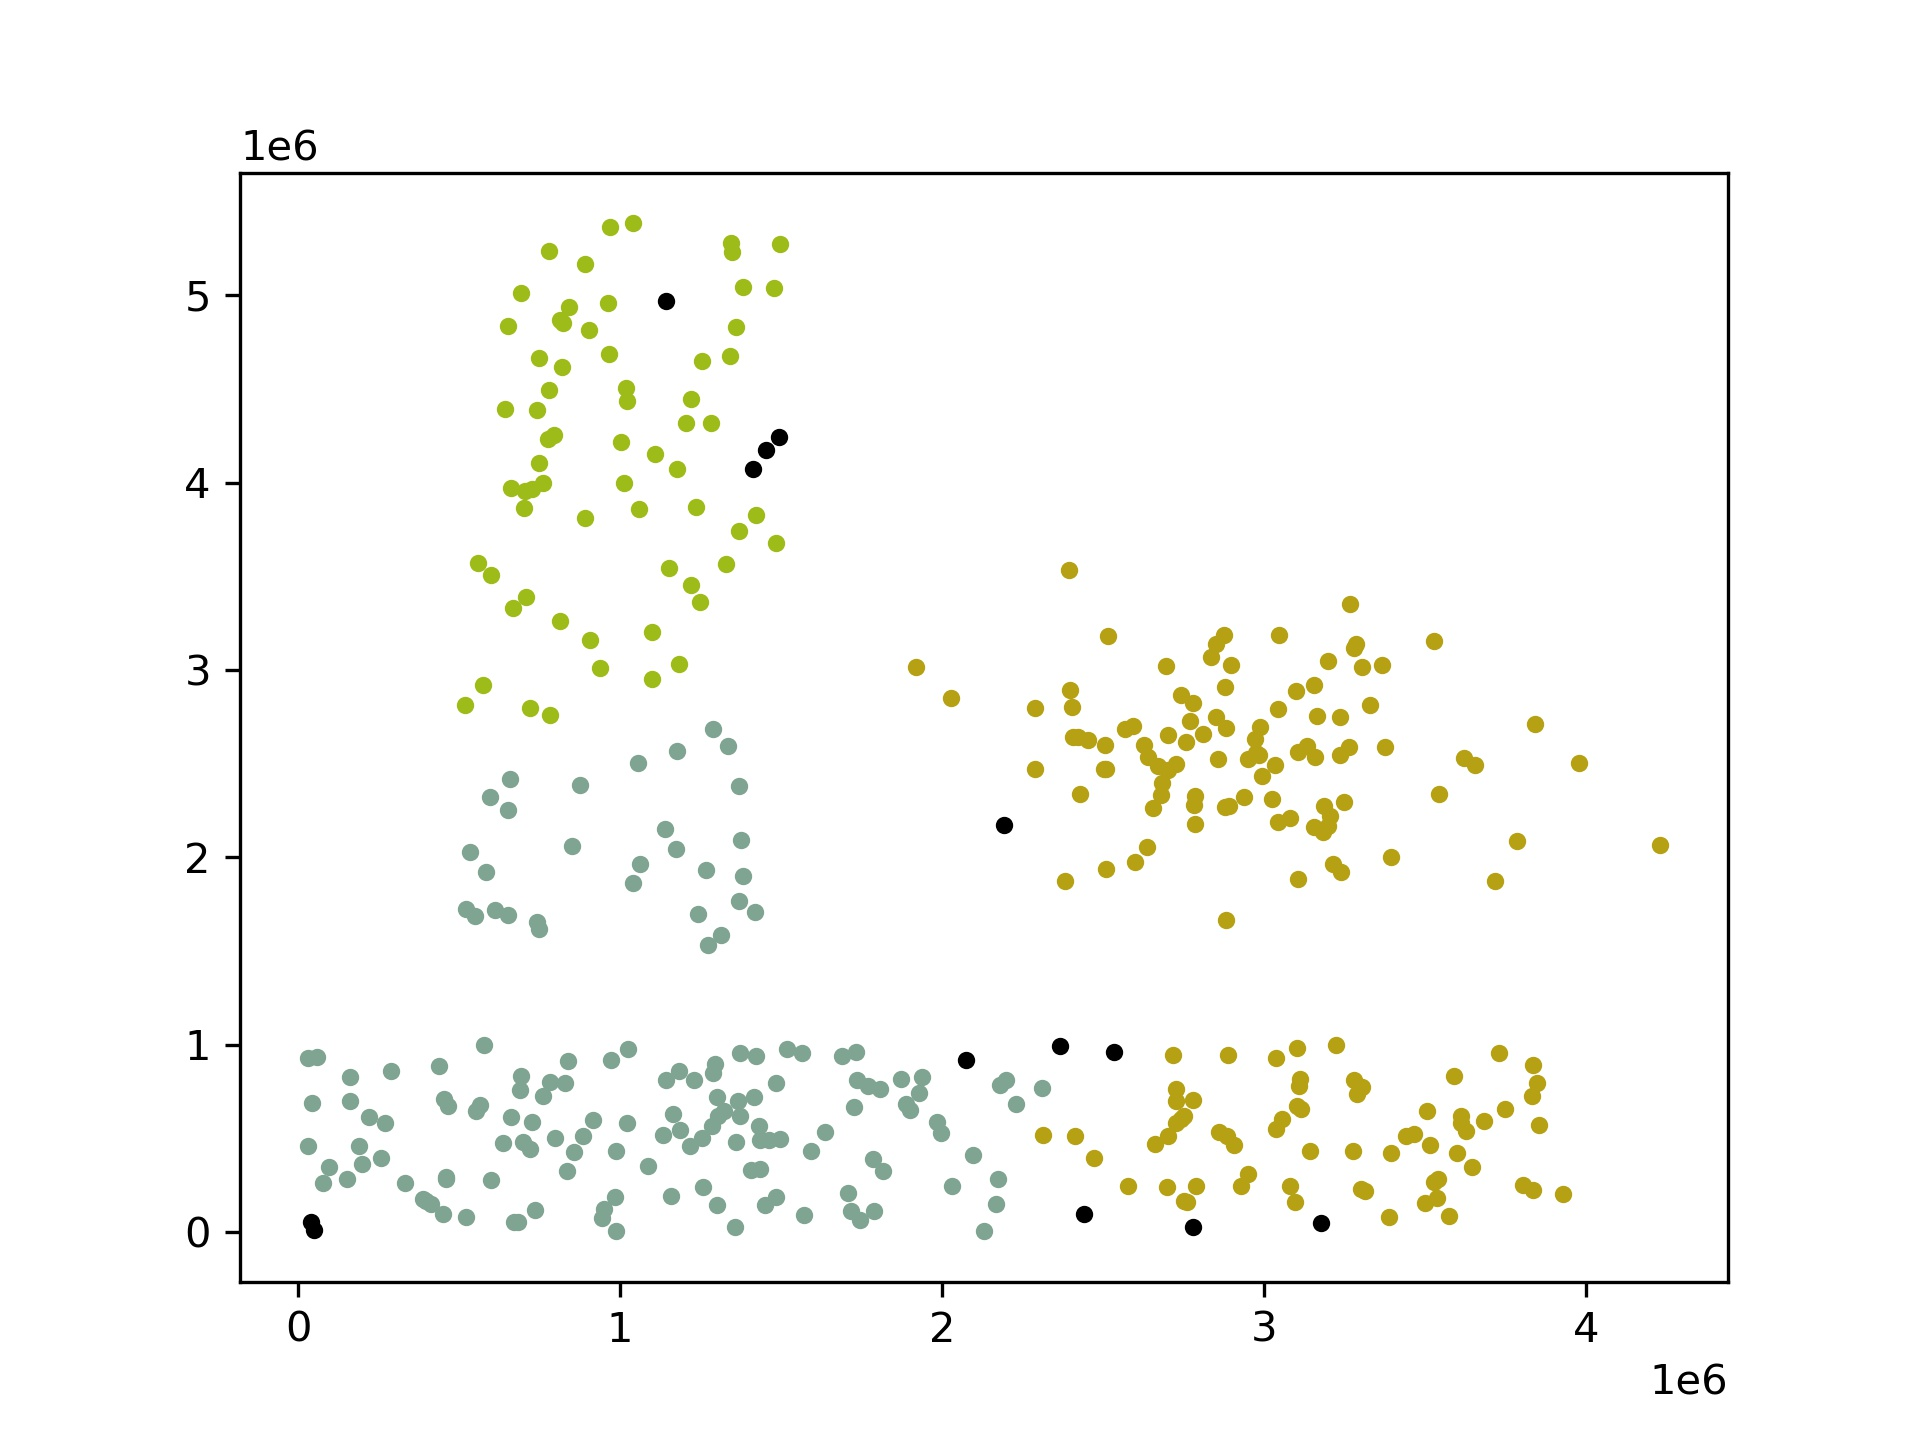
\includegraphics[width=.25\textwidth]{img/t3-lsun.jpg}}
	\subfloat[]{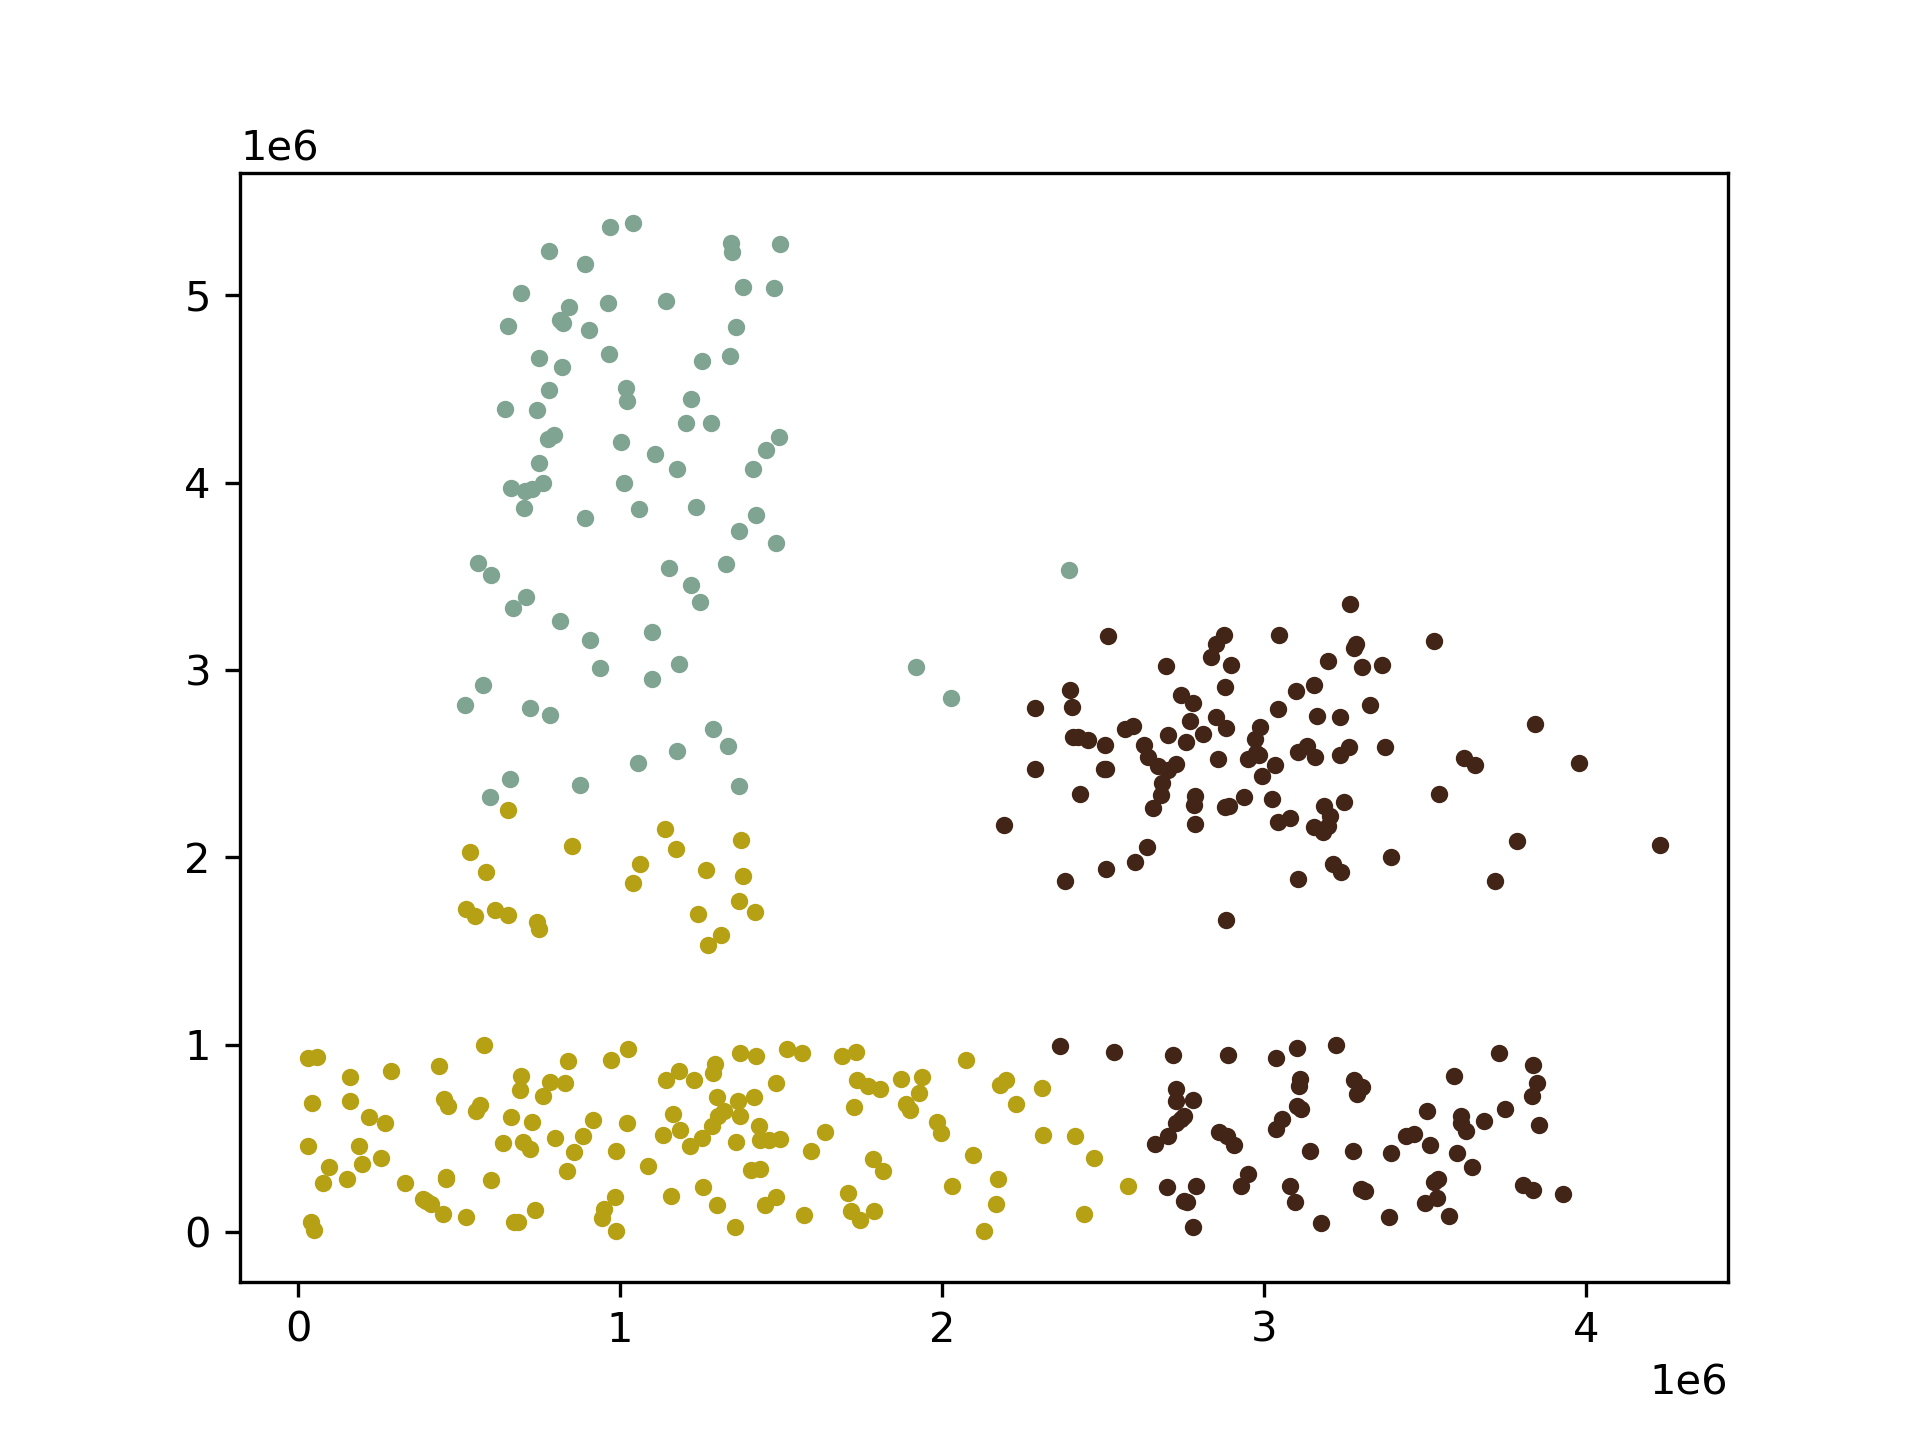
\includegraphics[width=.25\textwidth]{img/km-lsun.png}} \\
	\subfloat[]{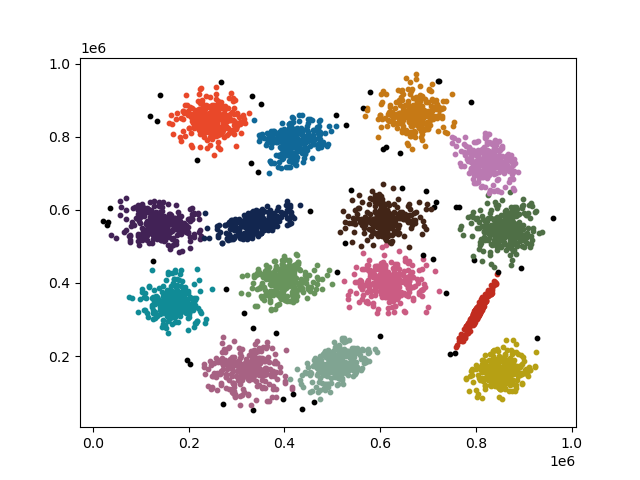
\includegraphics[width=.25\textwidth]{img/t1-s1.png}}
	\subfloat[]{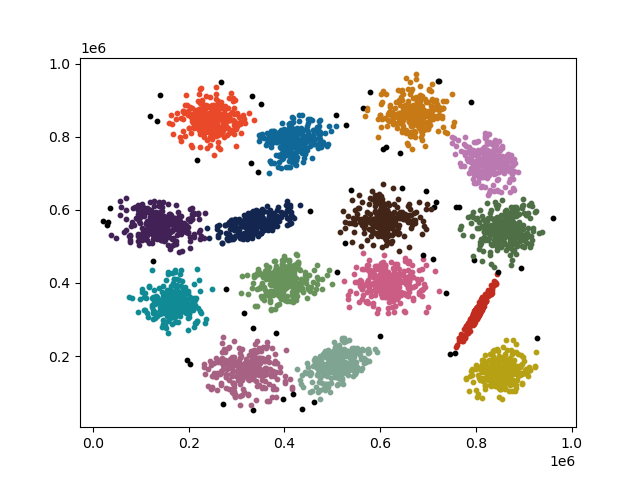
\includegraphics[width=.25\textwidth]{img/t2-s1.png}}
	\subfloat[]{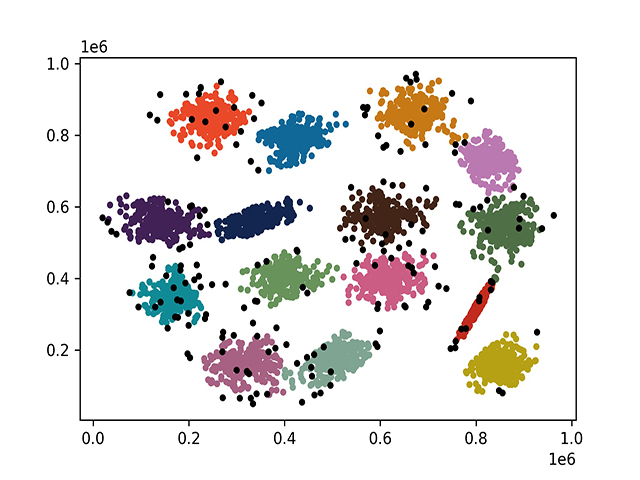
\includegraphics[width=.25\textwidth]{img/t3-s1.jpg}}
	\subfloat[]{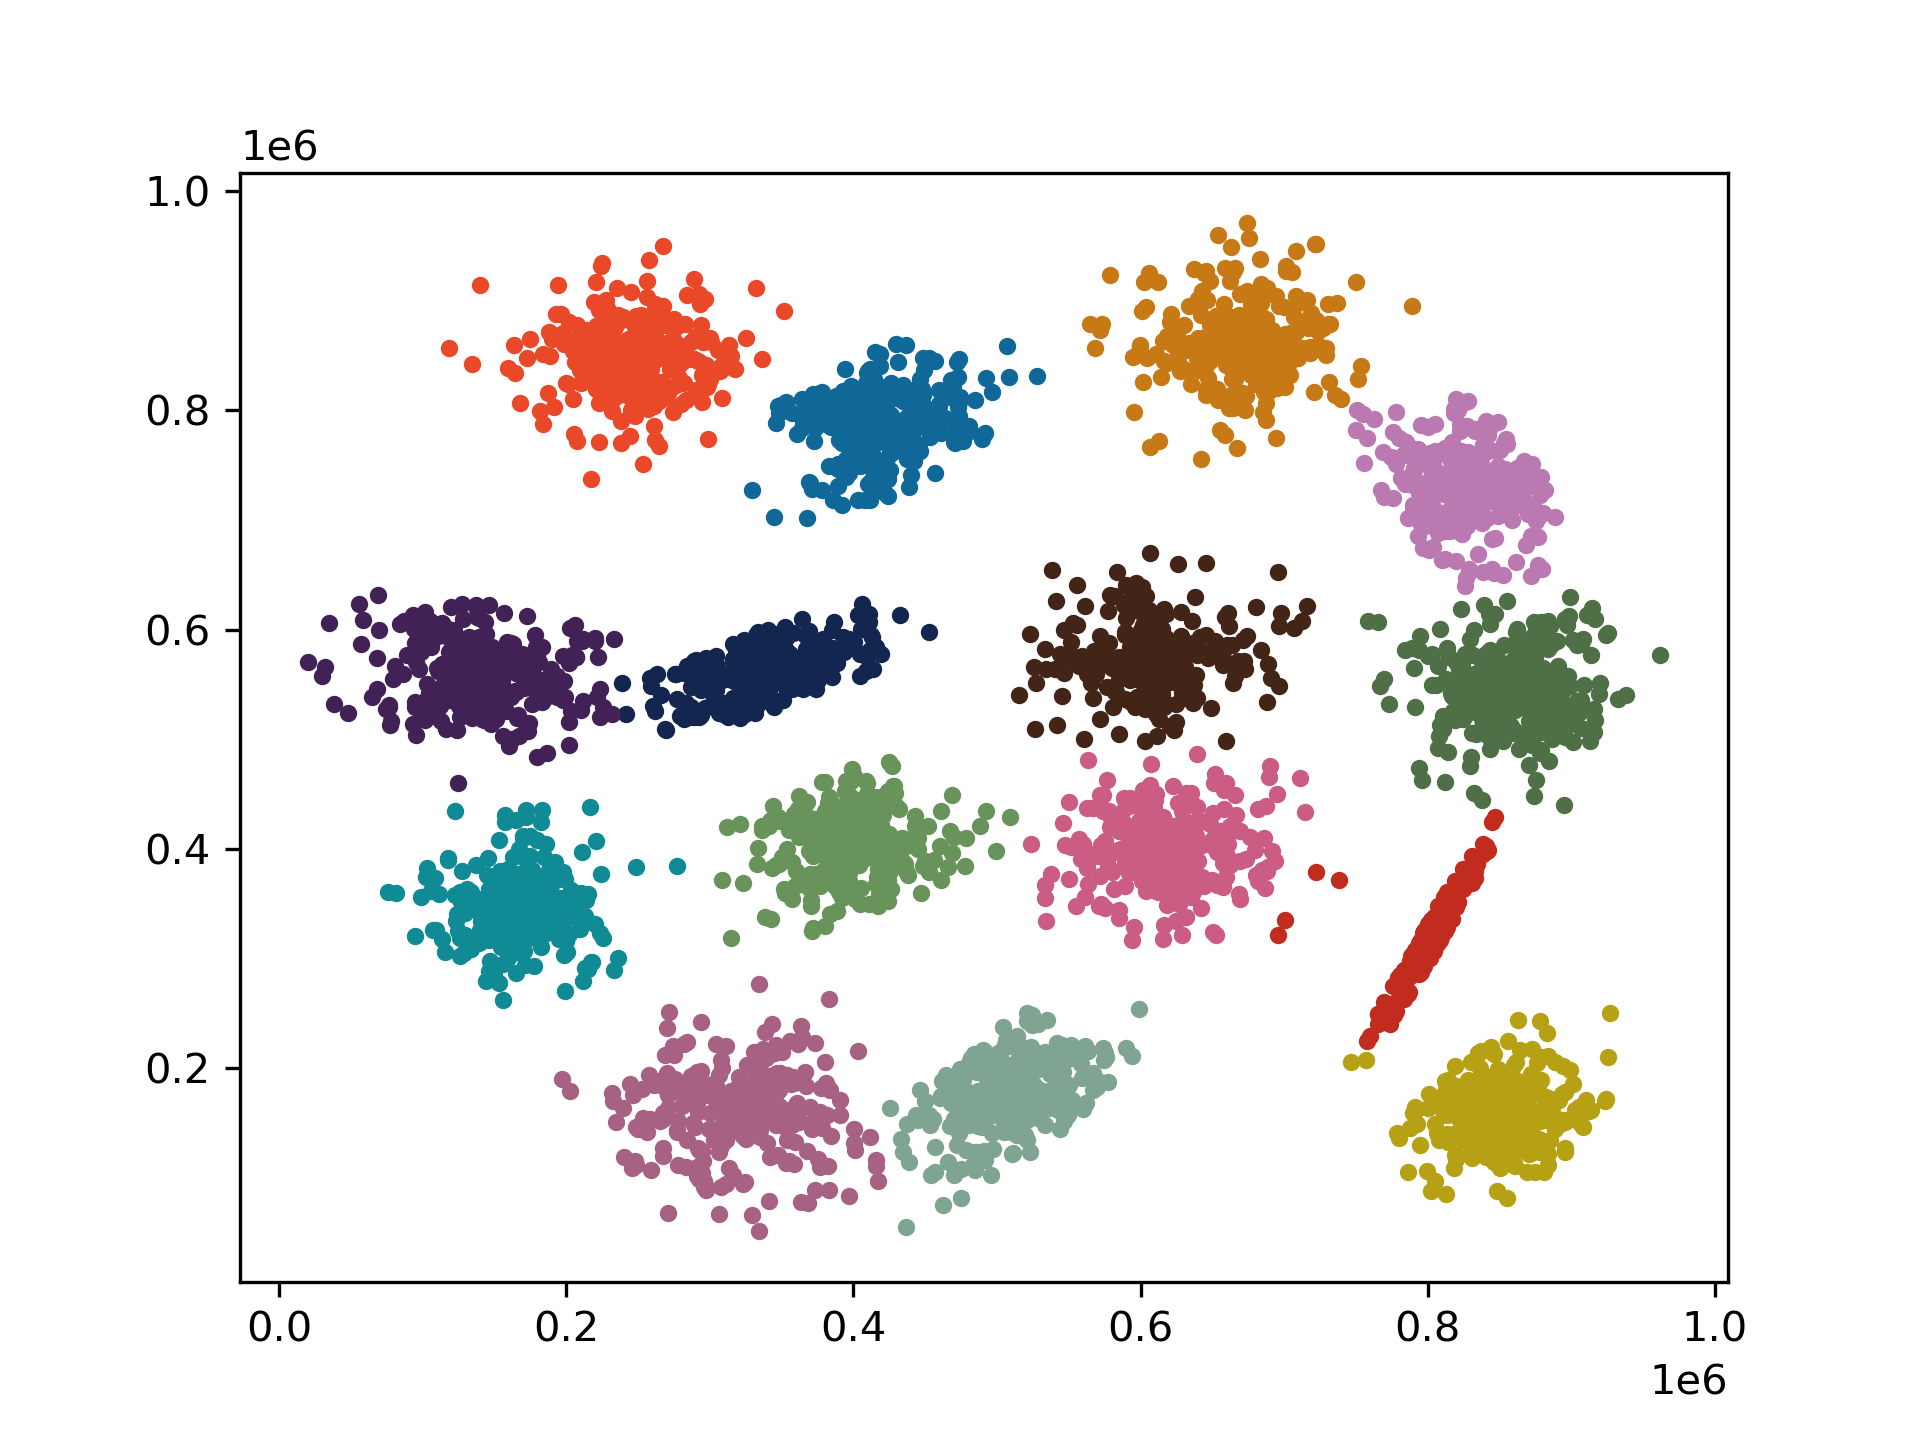
\includegraphics[width=.25\textwidth]{img/km-s1.png}}
	\\
	\subfloat[]{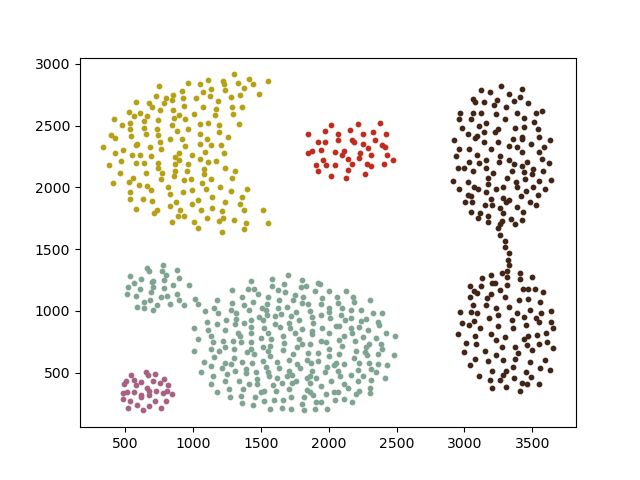
\includegraphics[width=.25\textwidth]{img/t1-aggre.png}}
	\subfloat[]{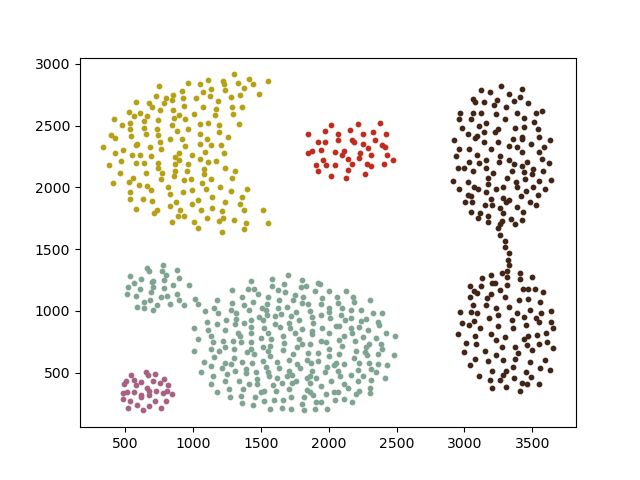
\includegraphics[width=.25\textwidth]{img/t2-aggre.png}}
	\subfloat[]{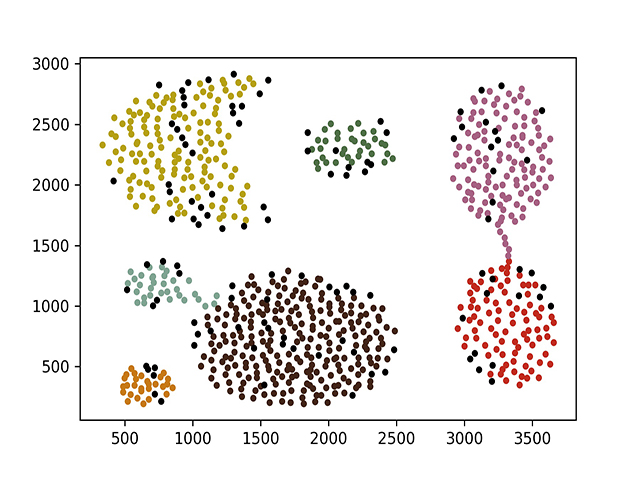
\includegraphics[width=.25\textwidth]{img/t3-aggre.jpg}}
	\subfloat[]{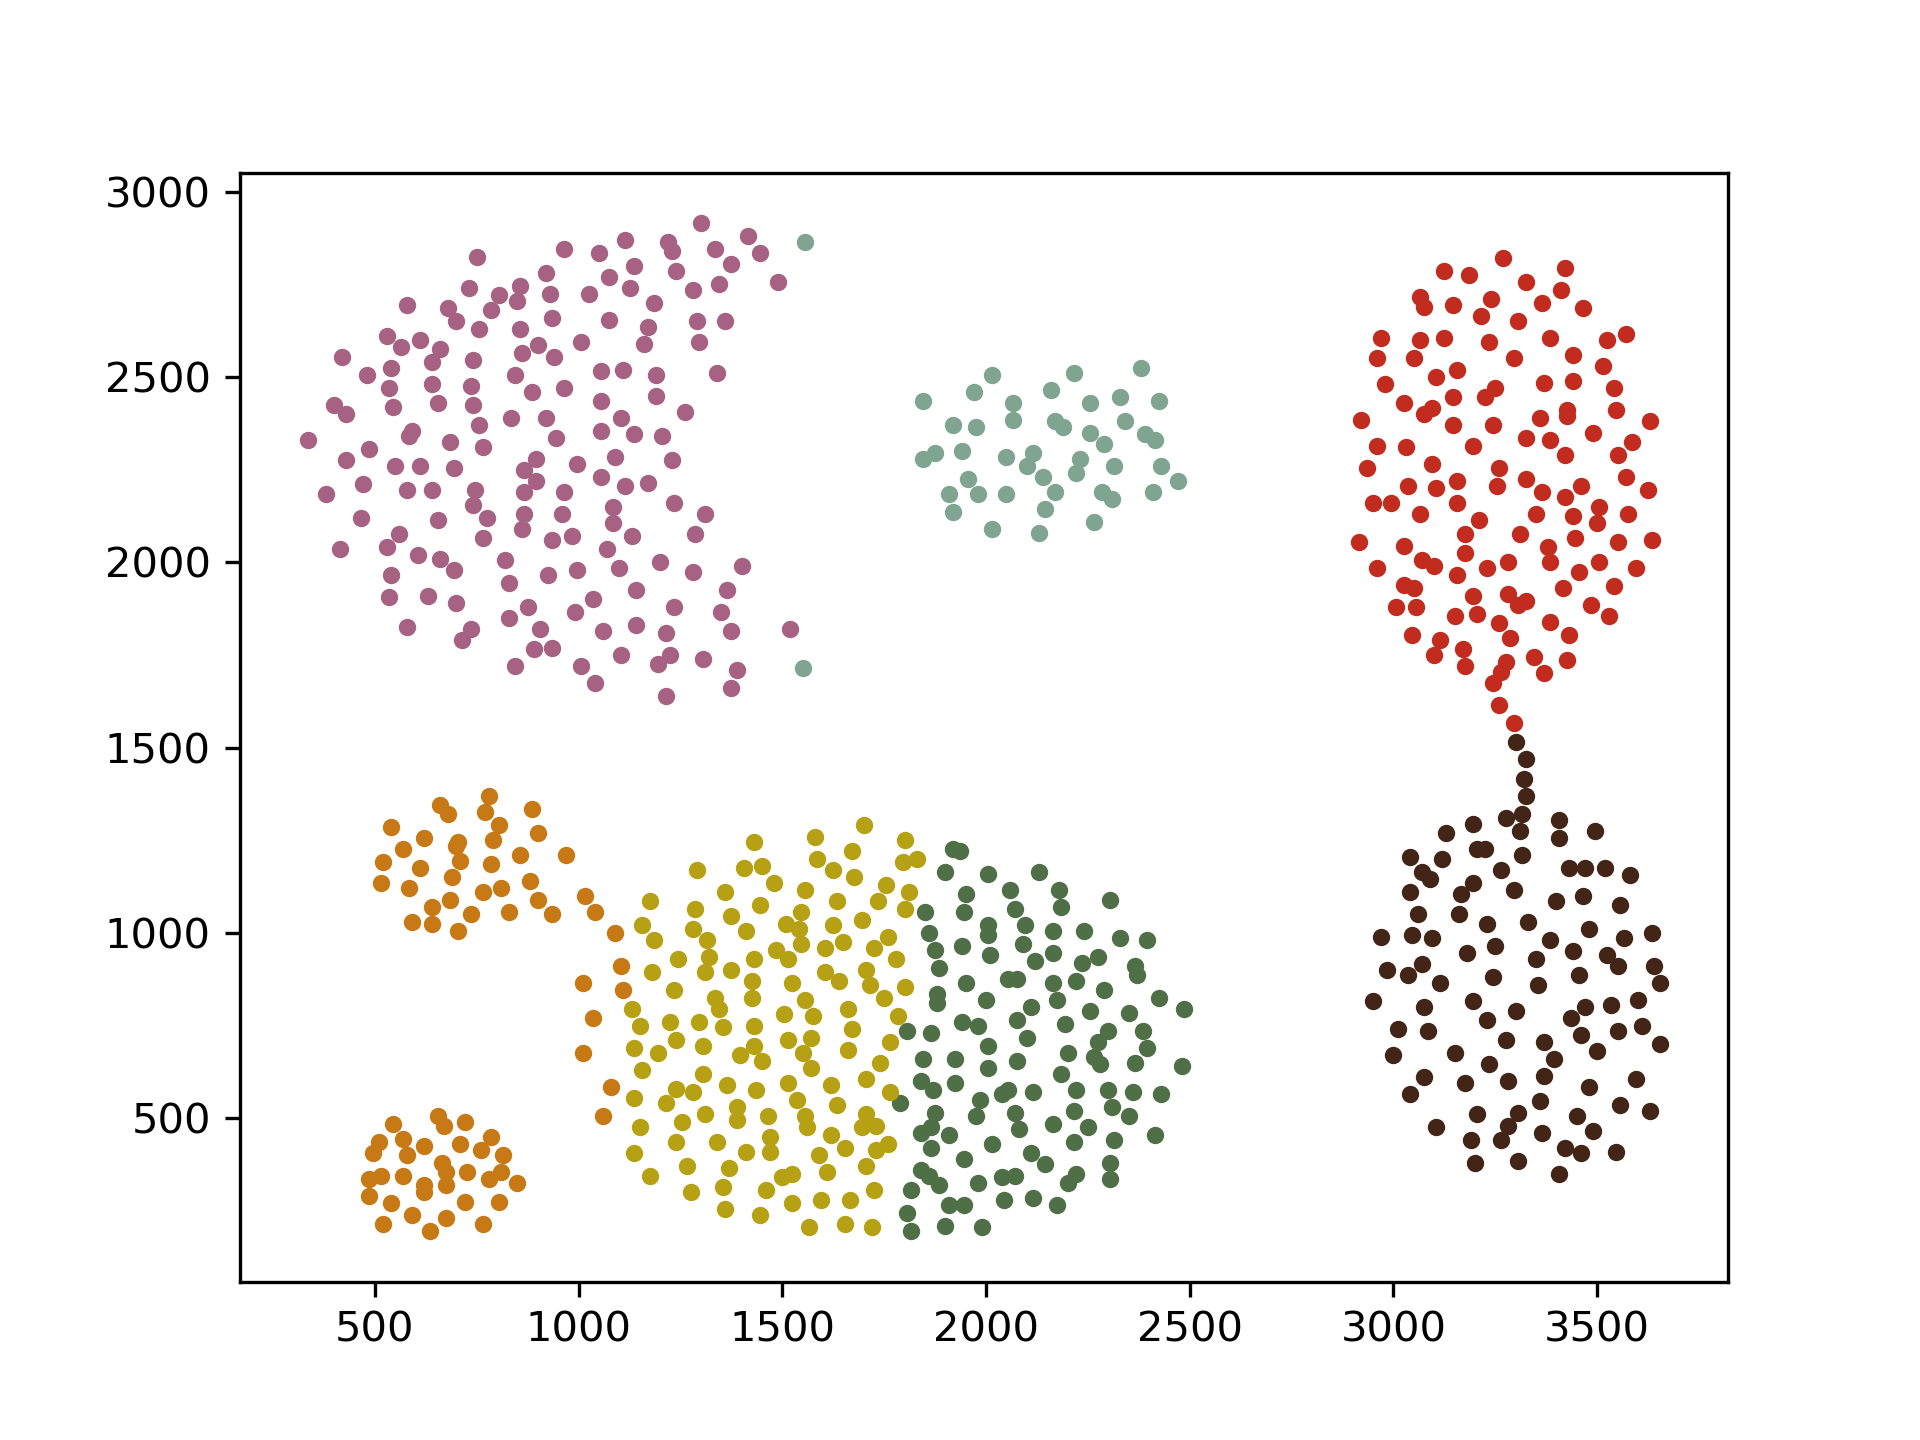
\includegraphics[width=.25\textwidth]{img/km-aggre.png}}
	\caption{聚类结果可视化比较}
	\label{s4-img-clures}
\end{figure}

\begin{figure}[htbp] %[htbp]
	\begin{minipage}[t]{0.33\linewidth}
		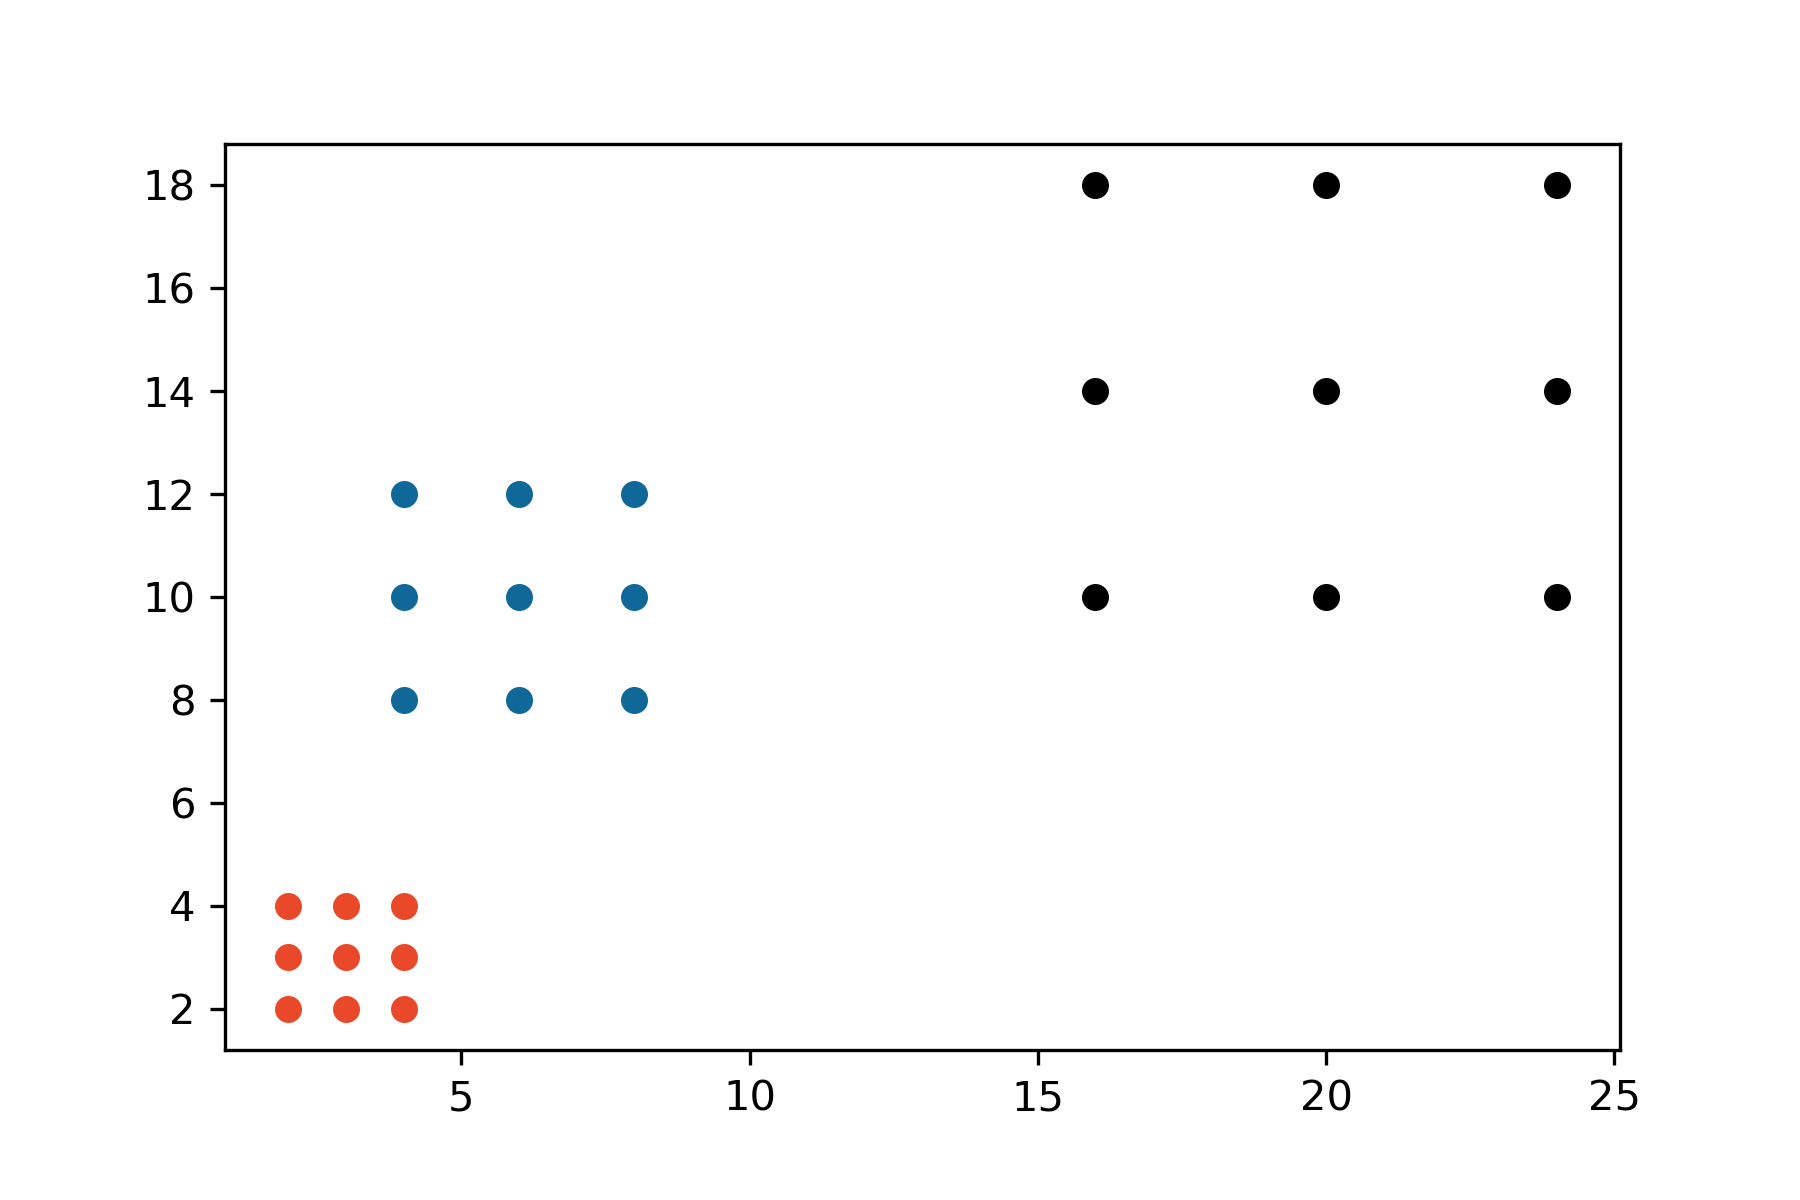
\includegraphics[width=\linewidth]{img/dbhc-exp-1.png}
		\caption{方案一($ \epsilon = 4 $)}
		\label{dbhcexp1}
	\end{minipage}%
	\hfill%
	\begin{minipage}[t]{0.33\linewidth}
		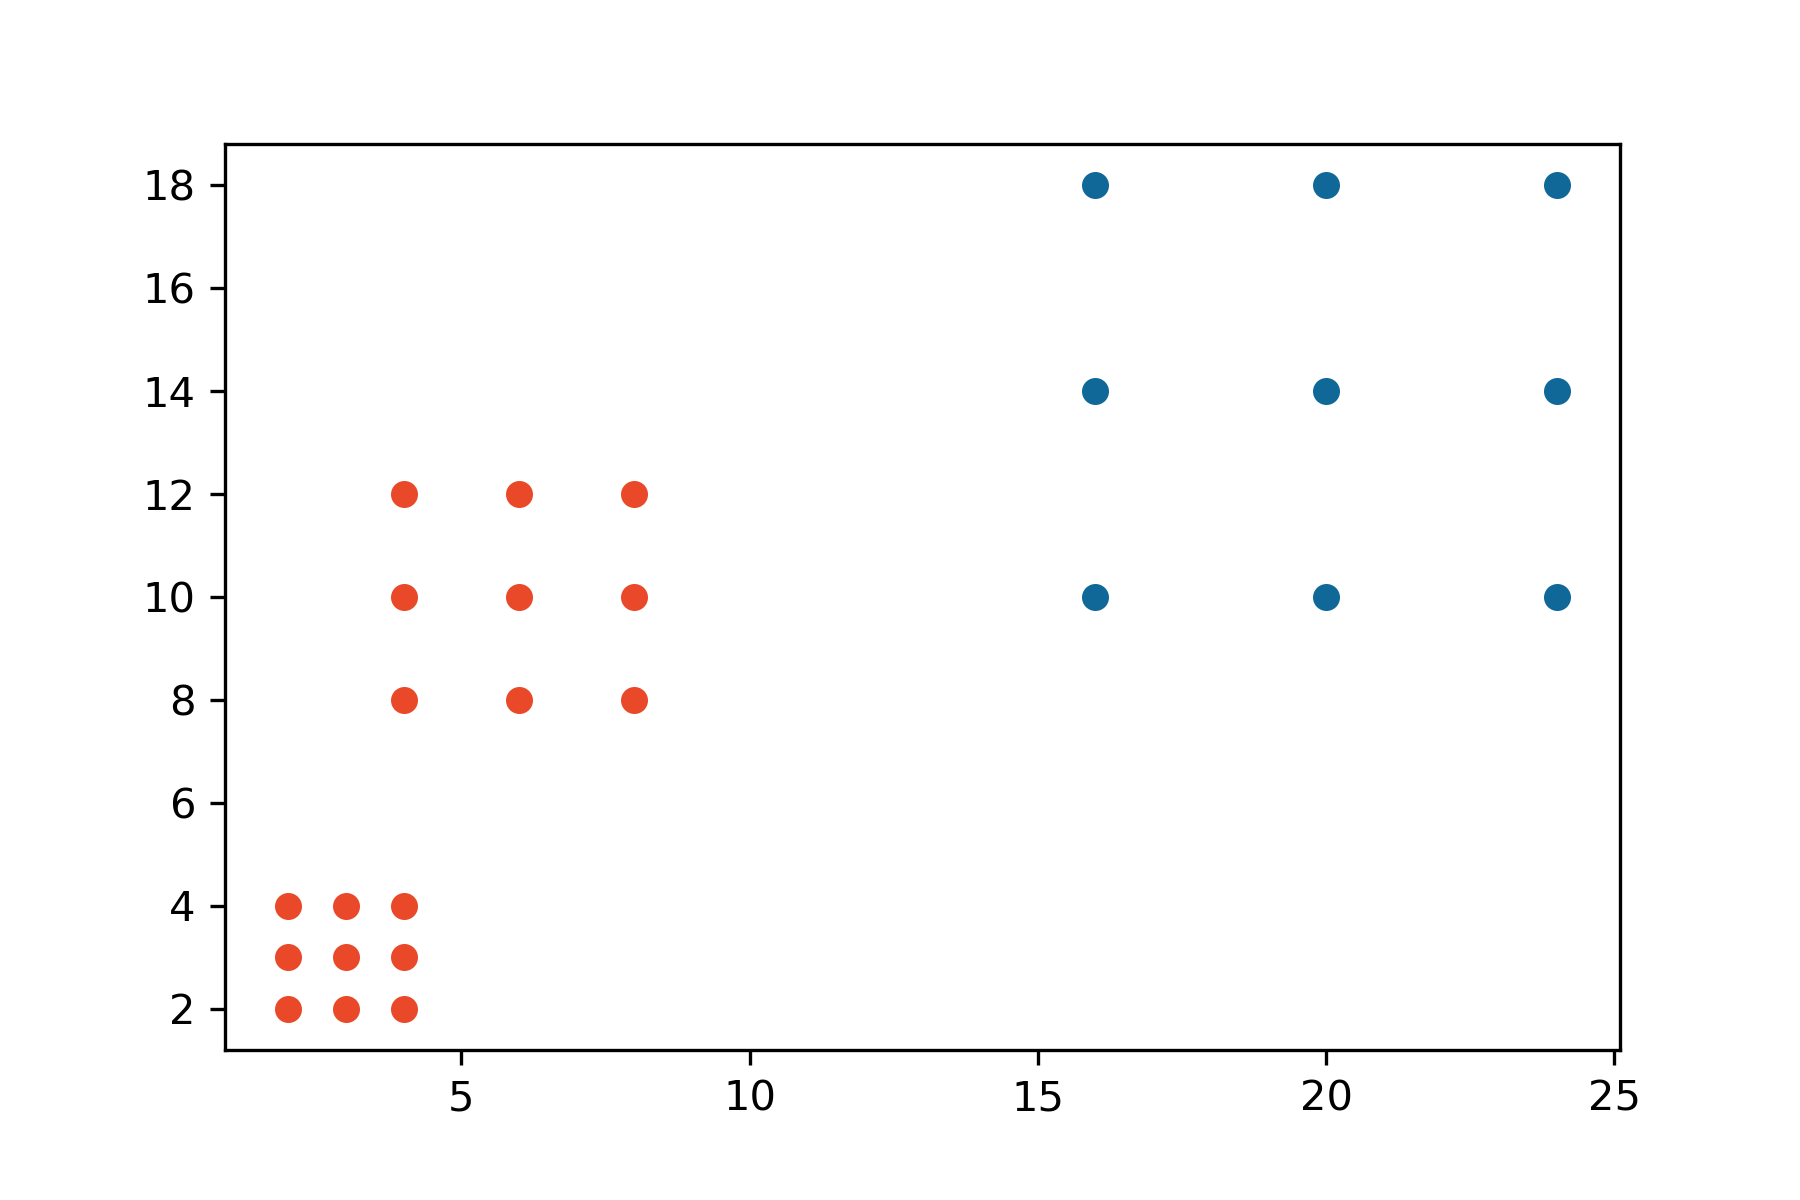
\includegraphics[width=\linewidth]{img/dbhc-exp-2.png}
		\caption{方案一($ \epsilon = 16 $)}
		\label{dbhcexp2}
	\end{minipage}
	\hfill
	\begin{minipage}[t]{0.33\linewidth}
		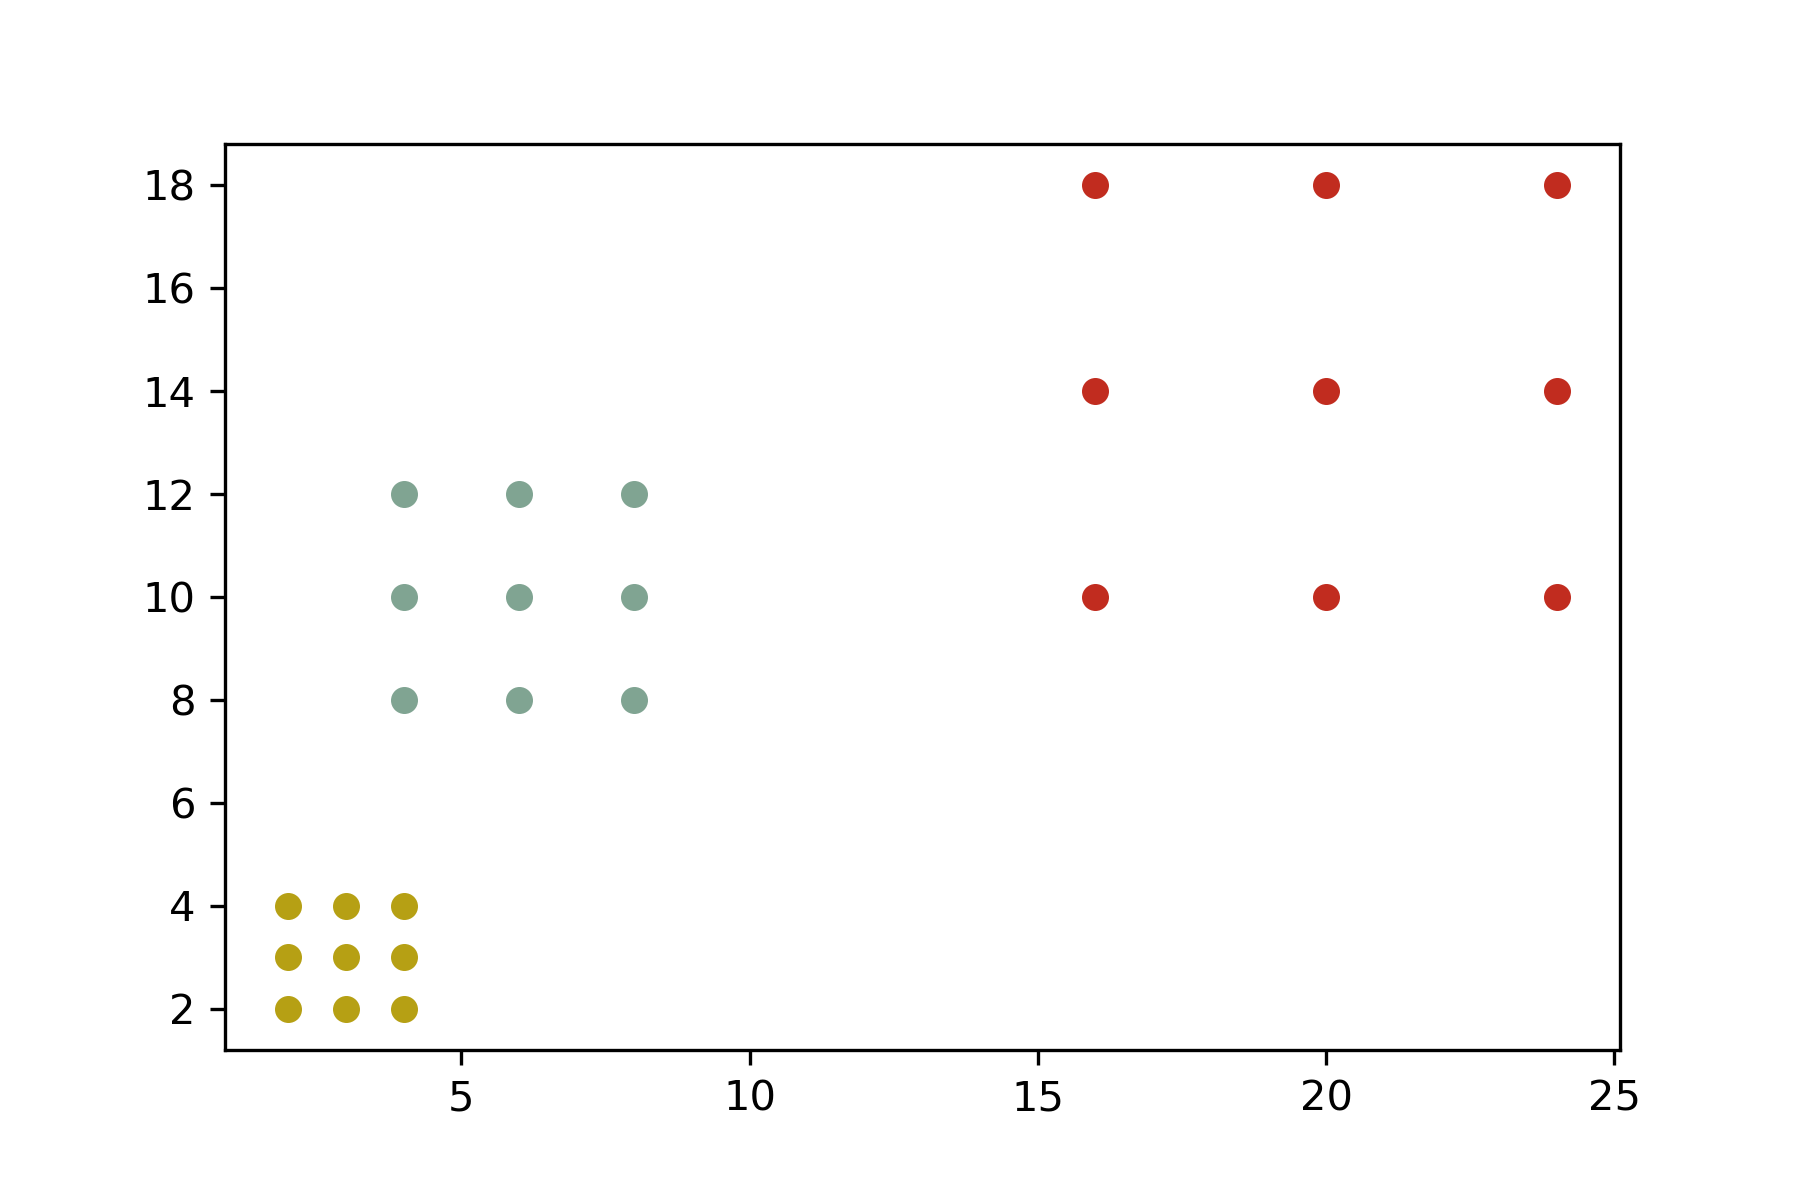
\includegraphics[width=\linewidth]{img/dbhc-exp-3.png}
		\caption{方案三(多$ \epsilon $值)}
		\label{dbhcexp3}
	\end{minipage}
\end{figure}

\textbf{多密度数据集聚类结果对比:}这里在人造数据集(如图\ref{fig:dd})上分别运行方案一和方案三。根据数据分布的特点,针对方案一需要手动设置$ \epsilon $,这里根据密度最大的簇C1,设置$ \epsilon $为4;根据密度最小的簇C3,设置$ \epsilon $为16。针对方案三,按照算法自动获取$ \epsilon $的值。对于minpts,设置为3。具体结果如下所示,图\ref{dbhcexp1}中的$ \epsilon $值适合密度较大的簇(即数据分布密集),C1和C2均能够被正确划分,C3则被划分为噪声点。图\ref{dbhcexp2}中,C3能够被正确划分,而C1和C2则被划分到同一个簇中。最后如图\ref{dbhcexp3}所示,方案三的划分结果和数据集真实划分情况完全一致。综上所述,方案三在多密度数据集上划分效果优于方案一和方案二。


\subsubsection{性能分析}
本小节,将详细讨论本文提出的系列隐私保护DBSCAN方案与隐私保护K-means方案\cite{mohassel2019practical}以及同类研究工作ppDBSCAN\cite{bozdemir2021privacy}的耗时对比。上述两个方案均较好的平衡了效率与安全,论文\cite{mohassel2019practical}在多方计算场景下提出了一种安全的高效隐私保护K-means方案,但是受限于K-means聚类本身的缺陷,聚类的效果较差,适用场景有限。而论文\cite{bozdemir2021privacy}所提出的方案虽然高效但是方案可能会存在轻微的数据泄露问题。其他隐私保护DBSCAN相关研究均存在较大的数据安全问题,同时没有给出具体的实现和详细的实验分析,因此这里不进行对比分析。

在表格\ref{s4-table-runtime}中,给出了上述方案在Lsun、S1和Aggregation数据集上的用时。其中论文\cite{mohassel2019practical}实验机器配置为Intel Core i7 2.6 GHz 12 GB RAM,模仿网络传输10Gbit/s和0.02ms的往返时间。而论文\cite{bozdemir2021privacy}的实验机器配置则是Intel Core i9-7960X CPUs 2.8 GHz 128 GB RAM,两个独立的服务器在10Gbit/s和0.02ms往返时间的网络上传输。两个方案的实验配置均与本实验的配置近似。此外,针对算法终止条件,K-means聚类在不同数据集上收敛所需迭代次数不同,论文\cite{mohassel2019practical}中给出的是算法迭代T次的总耗时数据,对于Lsun数据集设置T=15,而S1数据集则设置T=30。ppDBSCAN\cite{bozdemir2021privacy}与本文所述方案均统计算法从开始到结束所需时间。

\begin{table}[!htbp]
	\centering
	\renewcommand{\arraystretch}{1.3}
	\caption{耗时对比}
	\label{s4-table-runtime}
	\begin{tabular}{c|c|c|c|c|c}
		\hline
		隐私保护方案 & 隐私保护K-means聚类                      & \multicolumn{4}{c}{隐私保护DBSCAN方案}                                 \\
		\hline
		数据集       & Mohassel等人\cite{mohassel2019practical} & Bozdemir等人\cite{bozdemir2021privacy} & 方案一  & 方案二   & 方案三   \\
		\hline
		Lsun         & 22.21s(T=15)                           & 420.72s                                & 4 .12s  & 27.90s   & 2508.27s \\
		\hline
		S1           & 1472.6s(T=30)                          & 620,912.70s                            & 301.12s & 1002.55s & -        \\
		\hline
		Aggregation  & -                                        & -                                      & 103.77s & 639.10s  & 19620.2s \\
		\hline
	\end{tabular}
\end{table}

可以看到在所有数据集上,隐私保护DBSCAN方案(方案一)的耗时均最短,相较于论文\cite{mohassel2019practical}和ppDBSCAN分别有近5倍和100倍的提升,在耗时上远远优于其他高效的方案。
而改进的隐私保护DBSCAN方案(方案二)的耗时在Lsun数据集上则略逊色于论文\cite{mohassel2019practical},同时领先ppDBSCAN约14倍,方案二为了稳定聚类划分的结果引入了更多比较操作,因此耗时相对于方案一略有增加,但同时也提升了聚类质量。
方案三在耗时上没有显著优势,但是该算法的研究意义在于无需提供人工设定的参数$\epsilon$和minPts,减少了前置数据分析的工作量,使得算法的运行更加独立,并且能够更好的聚类多密度数据。


值得一提的是,K-means聚类收敛的速度受到数据集和初始簇中心的影响,若初始簇中心随机得到的结果较差,收敛所需迭代次数可能会增加。ppDBSCAN算法中提供的一种迭代终止策略也依赖于数据分布特点。本文所述的三种方案均无需考虑这些因素,聚类所需用时不受数据分布和初始簇中心选择的影响,方案耗时更加稳定。

接下来,根据图\ref{s4-exp-tcost}和图\ref{s4-exp-ccost}来对安全比较协议、安全极值协议以及安全排序协议从耗时和通信开销两个角度进行对比分析。
\begin{figure}[htbp] %[htbp]
	%	\captionsetup{font=scriptsize}
	\begin{minipage}[t]{0.5\linewidth}
		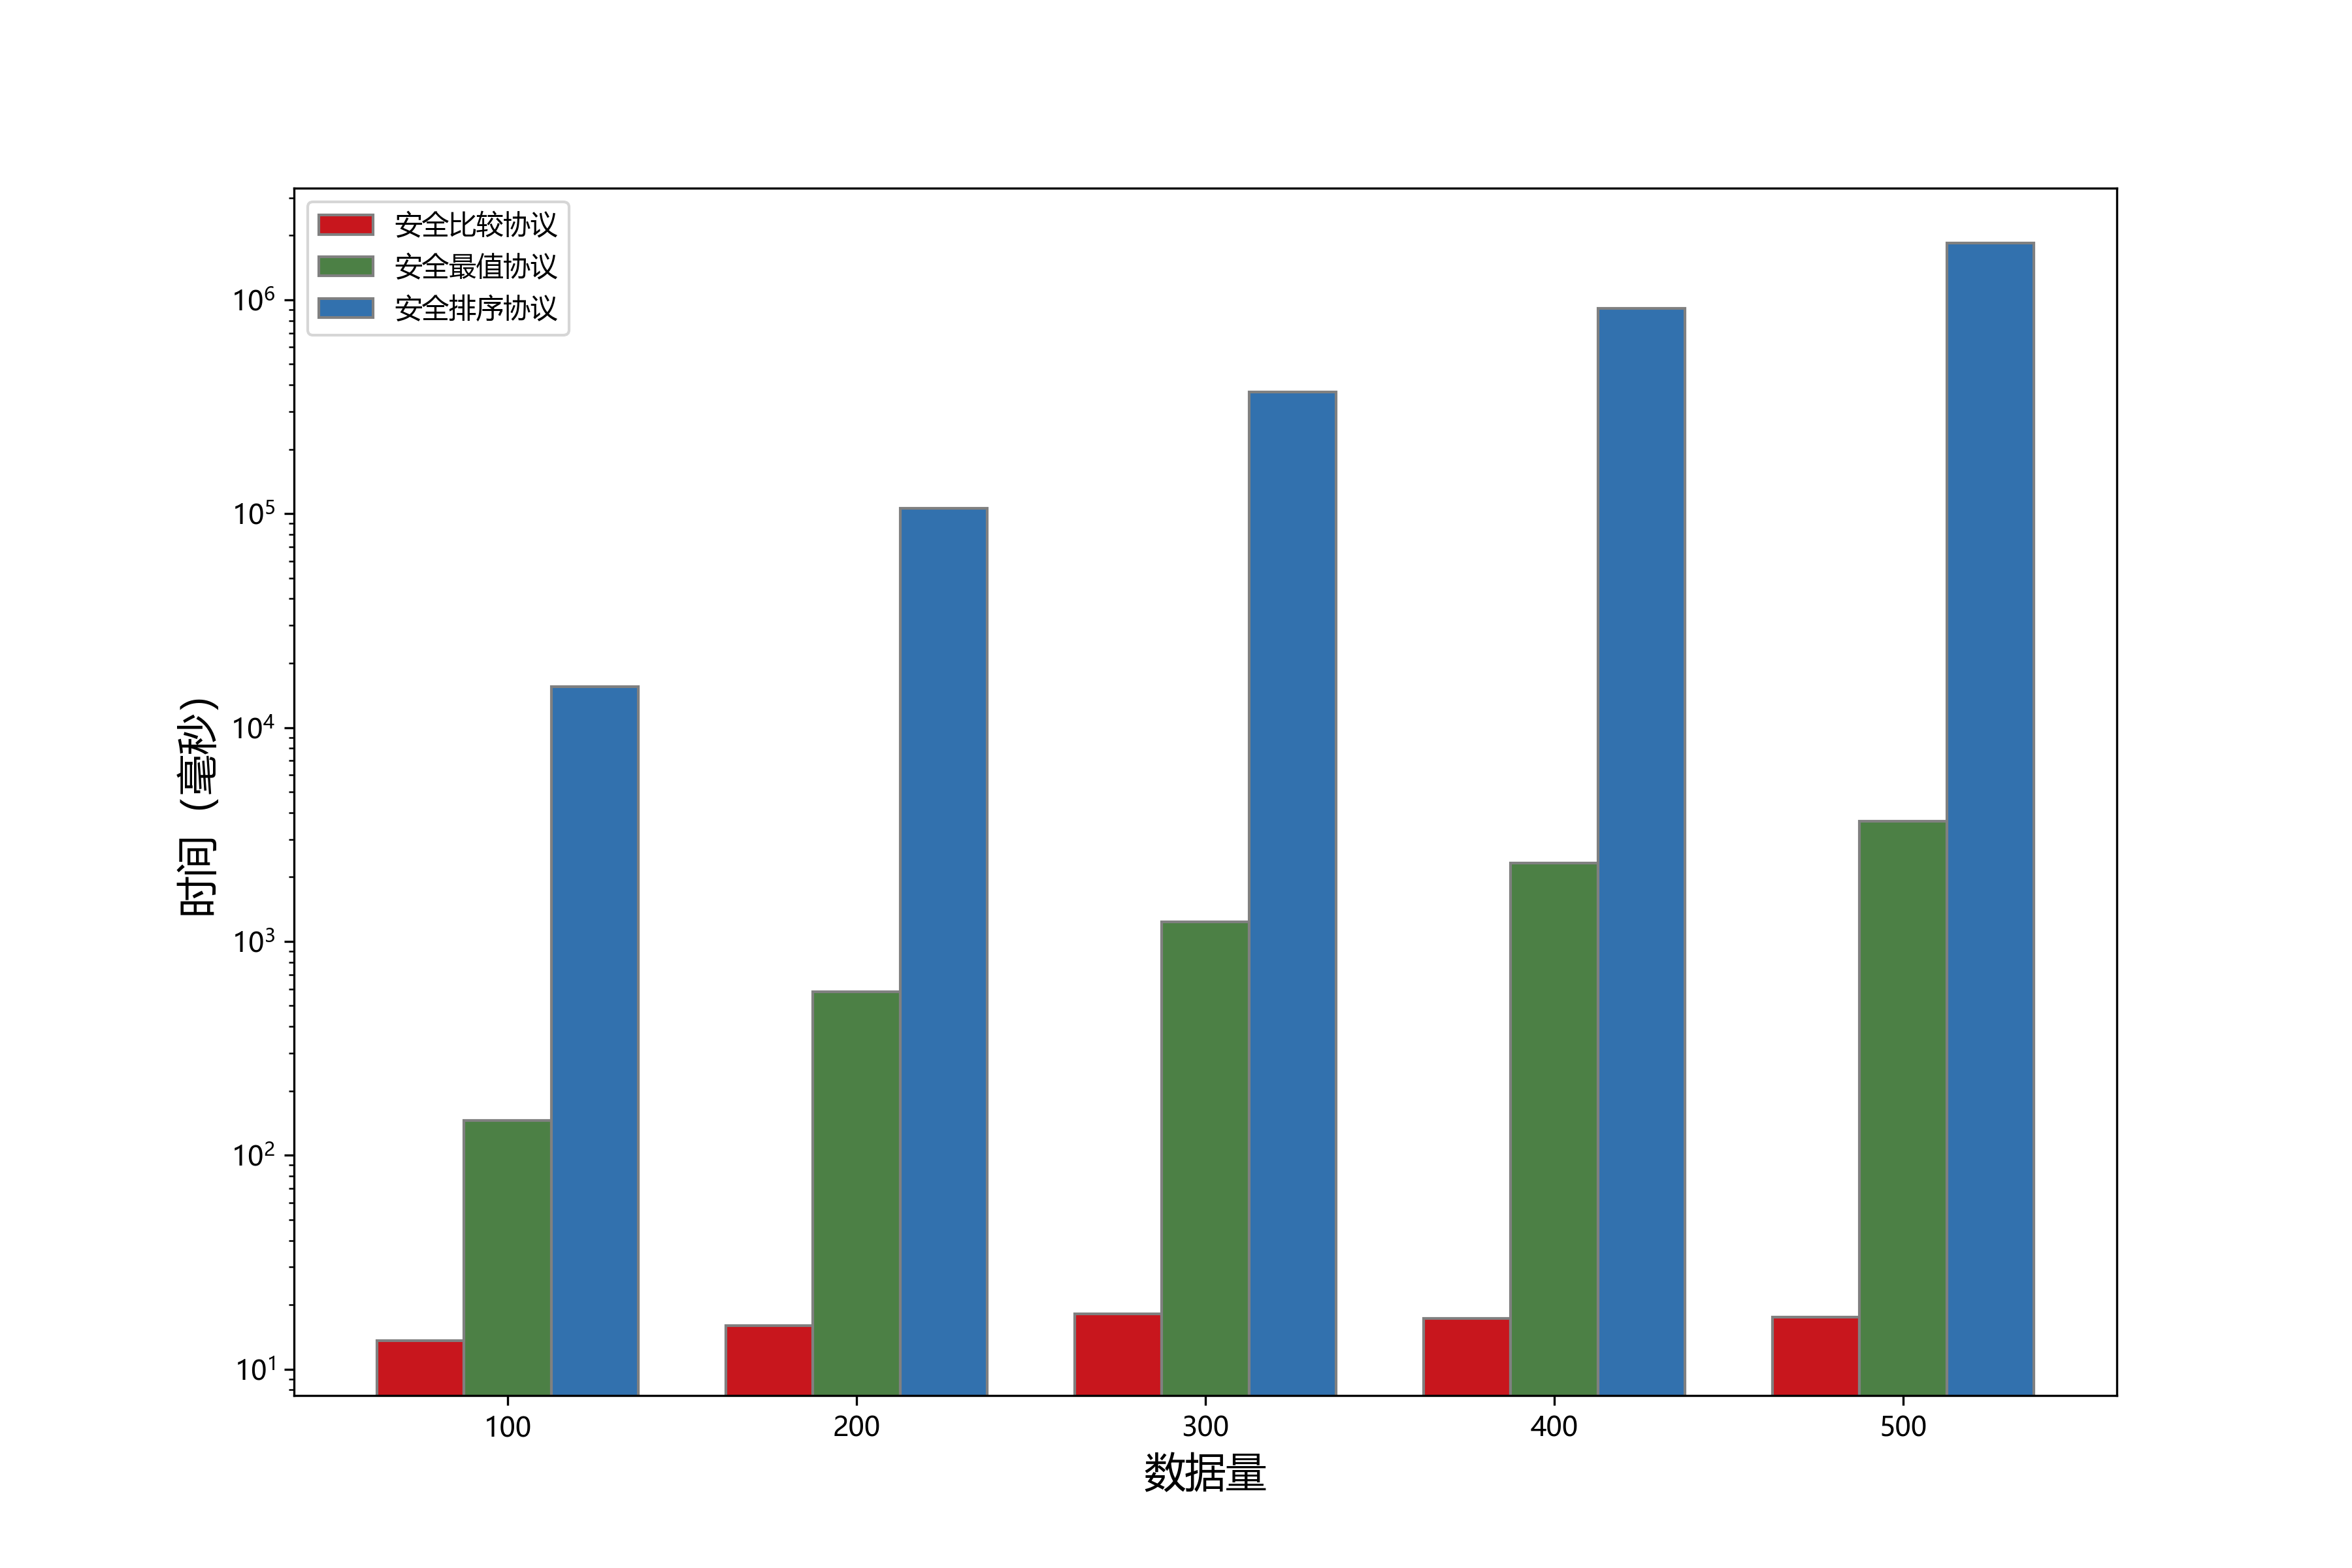
\includegraphics[width=\linewidth]{img/timecompare.png}
		\caption{耗时对比}
		\label{s4-exp-tcost}
	\end{minipage}%
	\hfill%
	\begin{minipage}[t]{0.5\linewidth}
		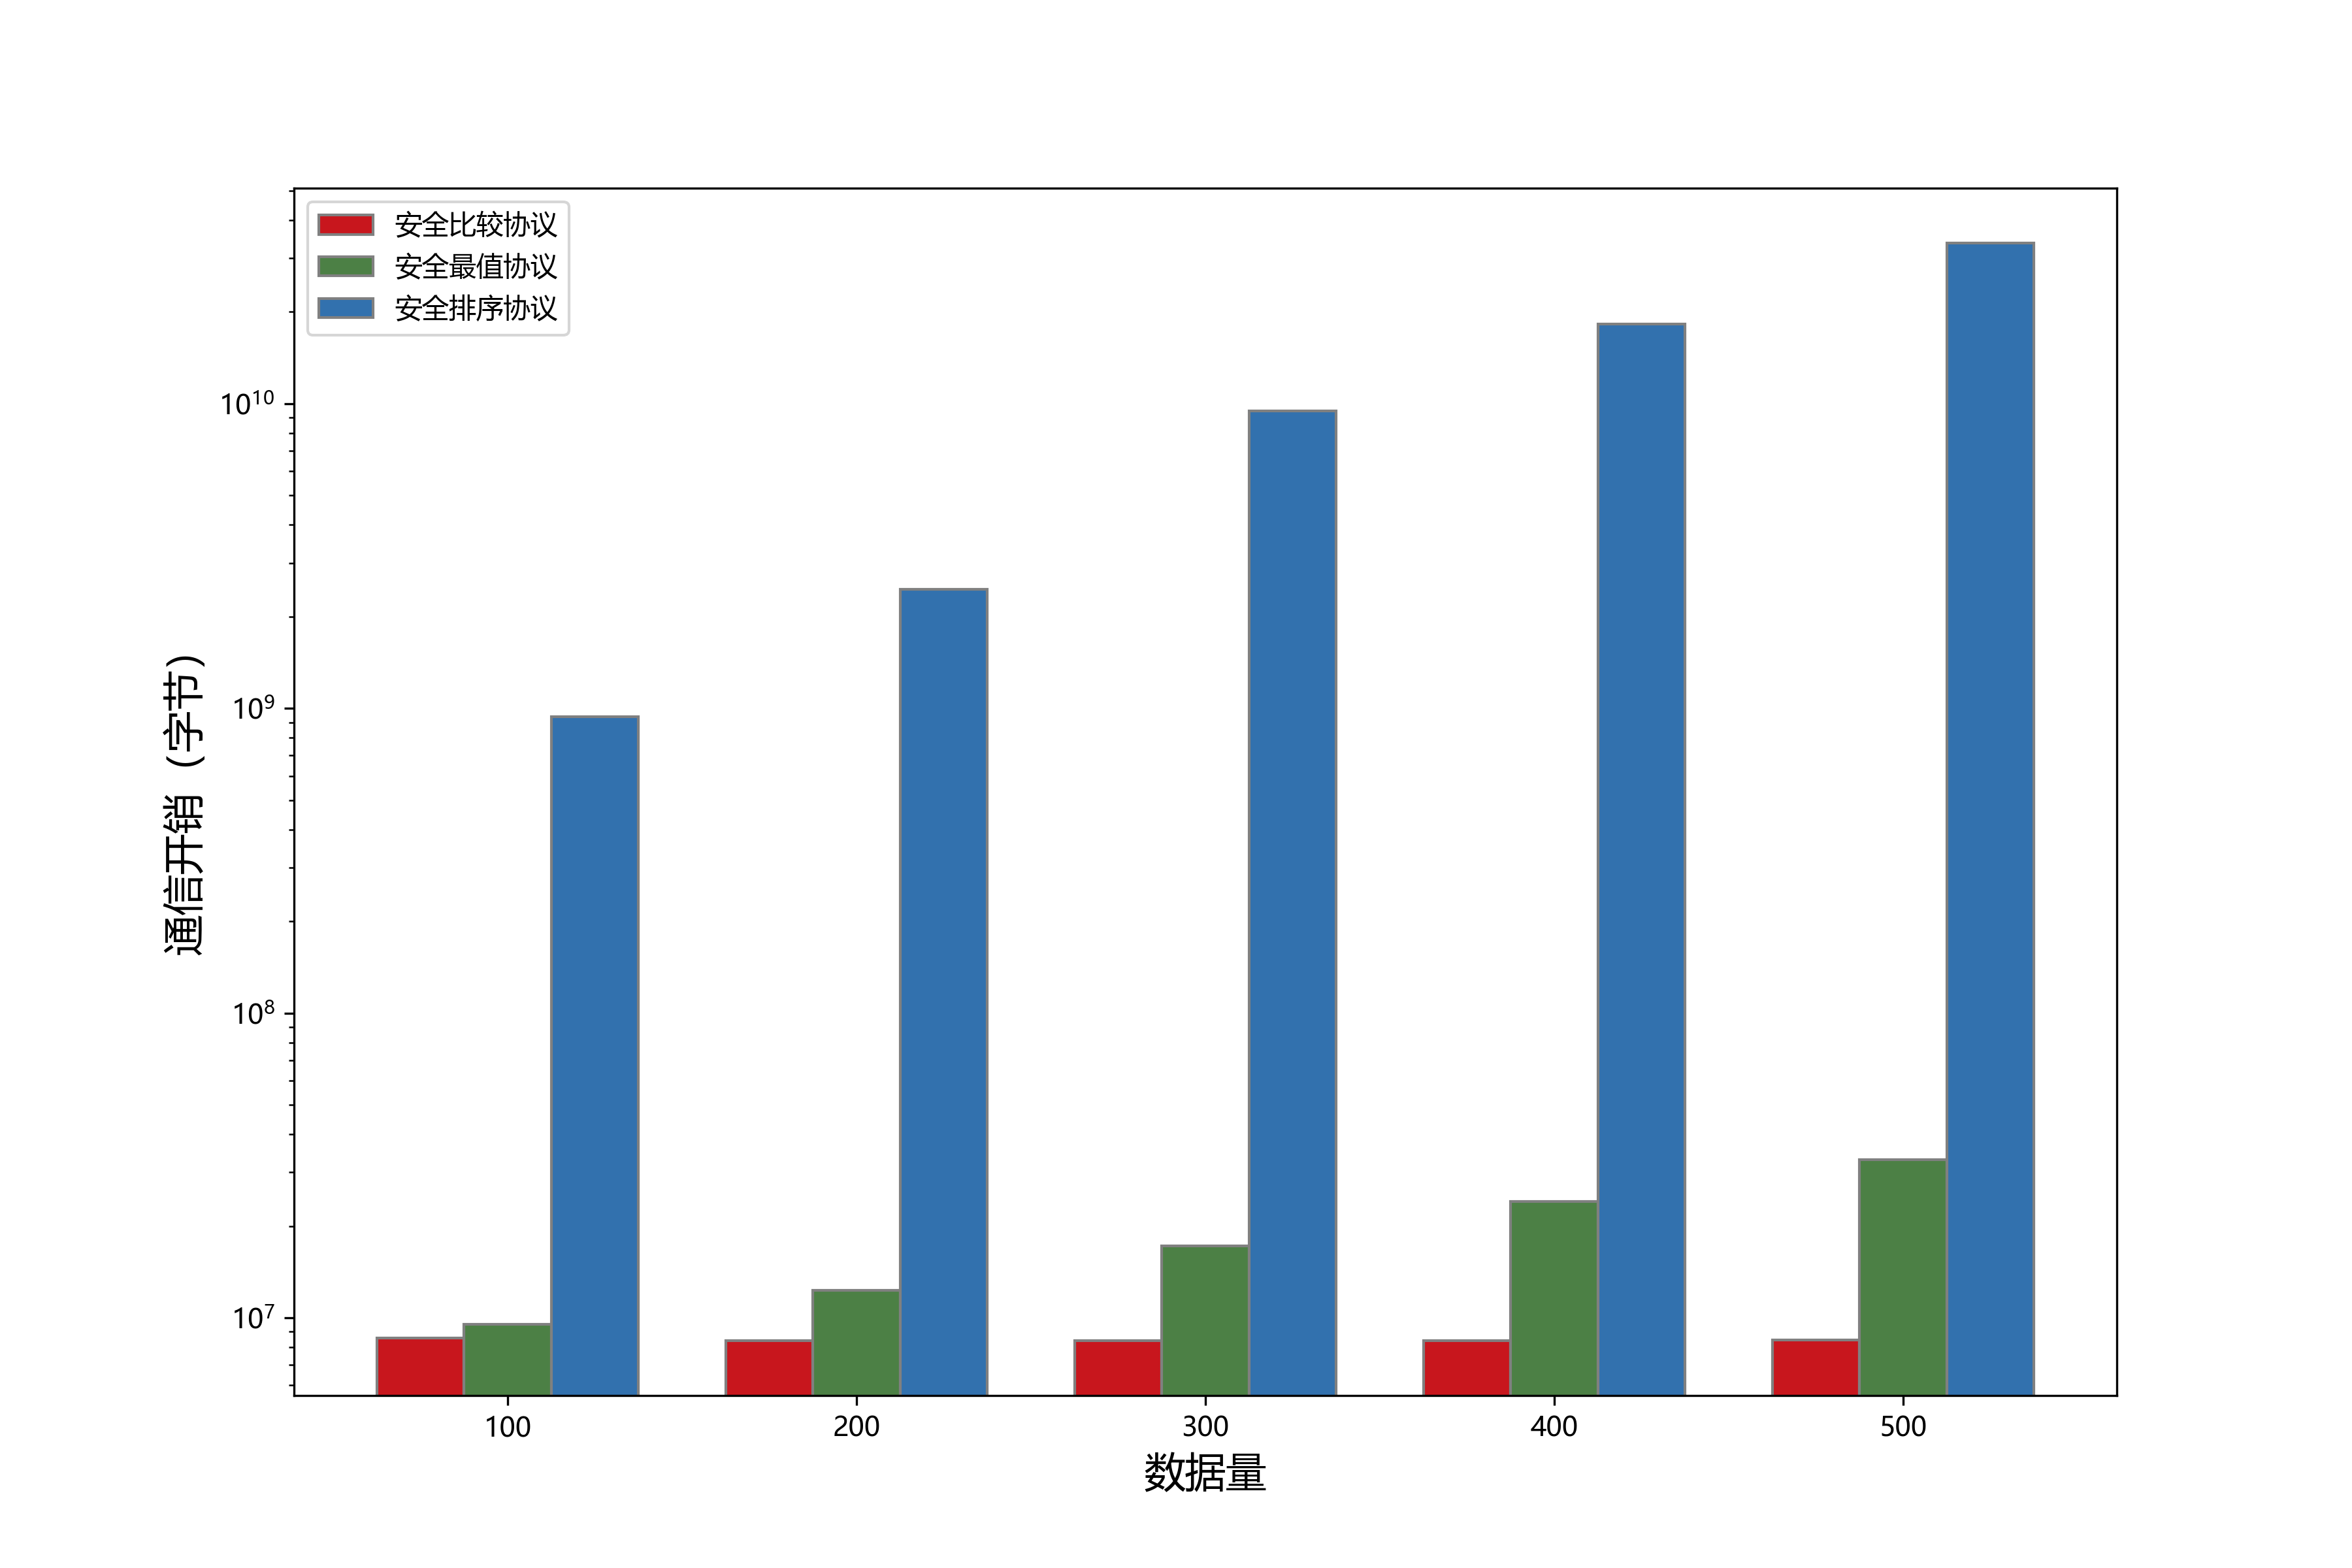
\includegraphics[width=\linewidth]{img/commcompare.png}
		\caption{通信开销对比}
		\label{s4-exp-ccost}
	\end{minipage}
\end{figure}

从图\ref{s4-exp-tcost}可以看到,三个协议随着数据量的增加耗时均有所增加,其中安全比较协议的耗时远远优于其他两个协议,主要原因是安全极值协议和安全排序协议由安全比较协议和其他操作组合而成,其中安全比较操作是性能瓶颈。

为了保证协议的顺利运行,设置数据传输的默认大小为$ 2^{20} $。在此基础上,可以看到安全排序协议的通信开销远超其他两个协议,原因在于对$ n $个数据进行安全排序,需要执行$ n $次安全极值协议,而每一次执行安全极值协议都需要进行一次安全比较,并行比较$ n(n-1) $对数据。
图中的变化规律可以反映上述关系,数据量的变化对安全比较协议耗费通信开销的增长速度影响较小,其他协议则不然。

综上所述,安全排序协议无论是从耗时还是通信角度,开销都非常大。在大数据上表现尤为明显,因此有其局限性。而安全比较协议和安全极值协议则表现较好,能够迁移到数量较大的场景中。
\begin{figure}[htbp]
	\centering
	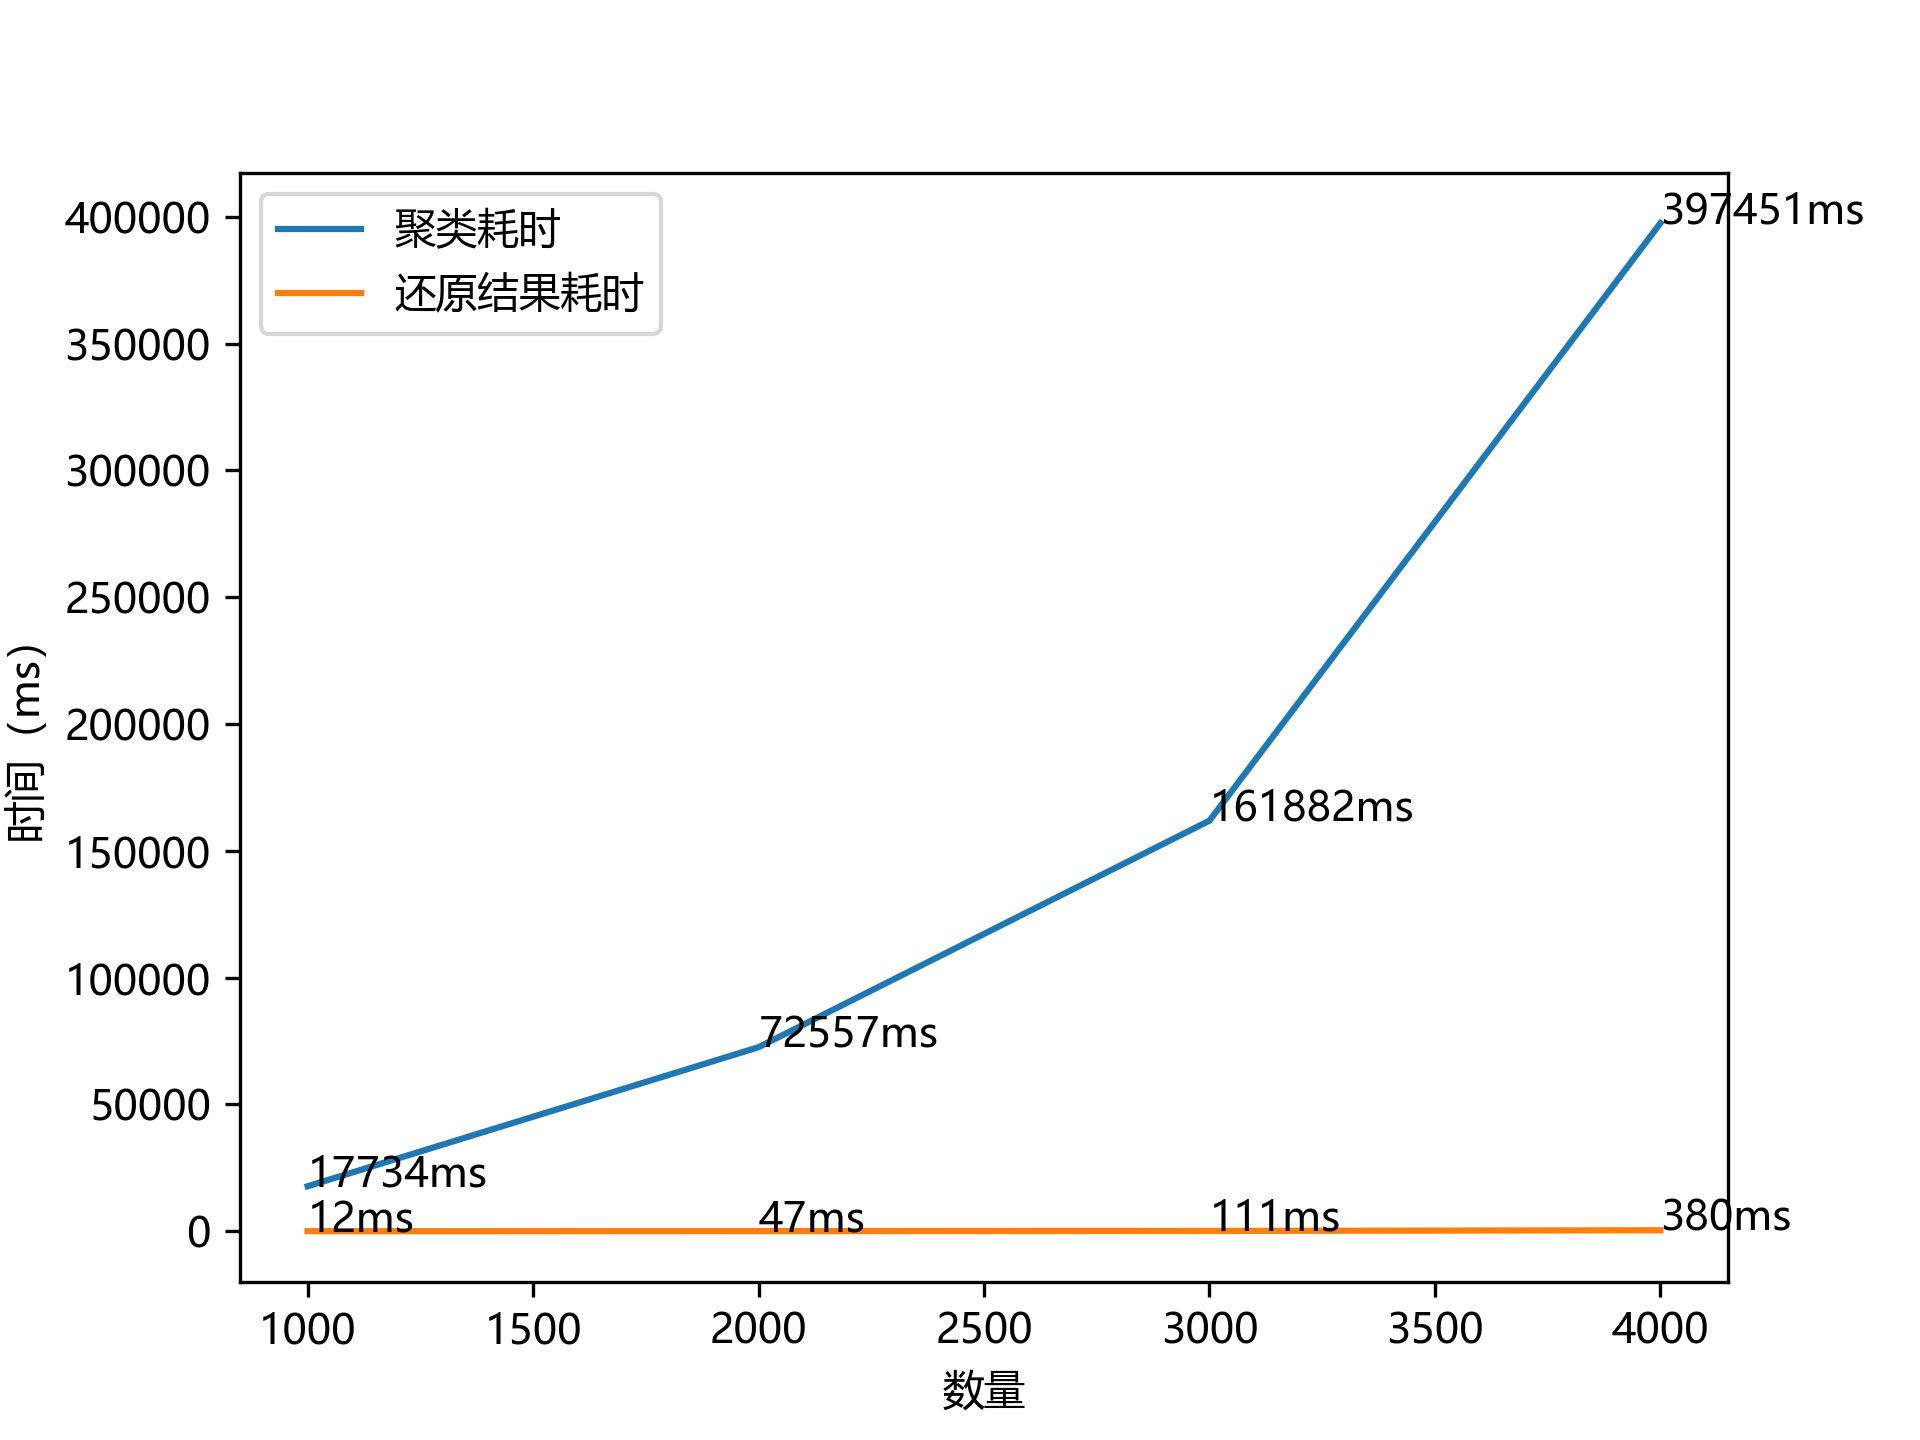
\includegraphics[width=0.6\linewidth]{img/testrc.png}
	\caption{聚类与还原结果耗时比较}
	\label{s4-exp-recover}
\end{figure}

最后简要分析,用户承担还原聚类结果的工作所需计算开销,如图\ref{s4-exp-recover}所示。
实验选择在数据量范围为$ [1000,4000] $的合成数据集上运行方案一获取耗时进行分析。
方案一与方案二的还原算法一致,方案三在原来算法的基础上,增加了合并初始簇的过程,计算比较简单,这里不进行单独分析。

可以看到还原结果所需时间显著低于聚类所需时间,特别是在数据量较大的情况下,差异更加明显。用户承担计算量的复杂度在$ O(n^2) $量级,因此认为隐私保护DBSCAN系列方案对用户带来的计算负担较小,能够帮助用户在保障数据安全的前提下,获取聚类结果。

\section{本章小结}
\label{s4-xiaojie}
现有的隐私保护DBSCAN相关研究相对隐私保护K-means聚类研究较少,许多研究不够完善,没有给出代码实现和实验分析。最近的同类方案\cite{bozdemir2021privacy}则存在数据泄漏风险,因此需要设计一个兼顾效率与安全的隐私保护DBSCAN聚类方案。

本章,从三个角度设计了系列安全高效的隐私保护DBSCAN方案。首先,基于传统DBSCAN的思想,对算法进行深入分析和改造设计了一种全新的密文聚类方式,聚类时获取临时簇并记录相连关系,最后根据深度优先遍历算法还原结果,该算法开销远低于论文\cite{bozdemir2021privacy}。
其次,为了解决DBSCAN中聚类划分结果不稳定的问题,提出了一种改进的隐私保护DBSCAN方案,该算法能够获取稳定的聚类结果以及提升聚类质量。
最后,为了减少对人工设置参数的依赖,提出了一个基于DBSCAN的隐私保护层次聚类方案,该方案无需根据数据分布设置关键参数,同时能够较好的聚类不同密度的数据。

%存在啥问题?方案三耗时较高,聚类效果有待提升;方案一和二
虽然本节的方案均兼顾了安全与高效,方案一和方案二具备良好的扩展性和可用性,在减少计算开销和提升聚类质量方面取得长足进展,但是方案三因其复杂性耗时较多,无法推广至大数据集,同时在某些数据集上聚类效果有劣势,仍需进一步改进,从多方面进行提升。